\def\filedate{2011/05/20}\let\thedate\filedate % packages may change \filedate

\documentclass[twoside]{article}
\usepackage[obeyspaces]{url}
\usepackage{natbib}
\usepackage{chem}
\usepackage{color}
\usepackage{rotating} % loads graphicx
%\usepackage{longtable}
\usepackage{graphicx}
%\usepackage{verbatim}

\oddsidemargin-5mm
\evensidemargin-5mm
\topmargin-10mm
\textheight230mm
\textwidth170mm
\raggedbottom
\parindent0mm
\parskip1.0ex plus0.5ex minus0.5ex
\renewcommand{\arraystretch}{1}
\renewcommand{\topfraction}{0.95}
\renewcommand{\dbltopfraction}{0.95}
\renewcommand{\bottomfraction}{0.95}
\renewcommand{\floatpagefraction}{0.95}
\renewcommand{\dblfloatpagefraction}{0.95}
\renewcommand{\textfraction}{0.01}
\setcounter{topnumber}{3}

\newcommand{\egcite}[1]{\citep[e.g.][]{#1}}
\newcommand{\etccite}[1]{\citep[and references therein]{#1}}
\newcommand{\hhline}{\noalign{\vspace{1mm}}\hline\noalign{\vspace{1mm}}}
\newcommand{\hhlines}{\noalign{\vspace{1mm}}\hline\hline\noalign{\vspace{1mm}}}
\newcommand{\kpproot}{{\sc root}}
\newcommand{\todo}[1]{{\uppercase{\bf ((#1))}}}
\newcommand\TODO[1]{\textcolor{red}{#1}}
\def\mypageheader{A. Kerkweg and P. J\"ockel: MMD Library Manual}
\markboth{\mypageheader}{\mypageheader}
\pagestyle{myheadings}

\begin{document}

\thispagestyle{empty}
\vspace*{-1.5cm}
\begin{center}
 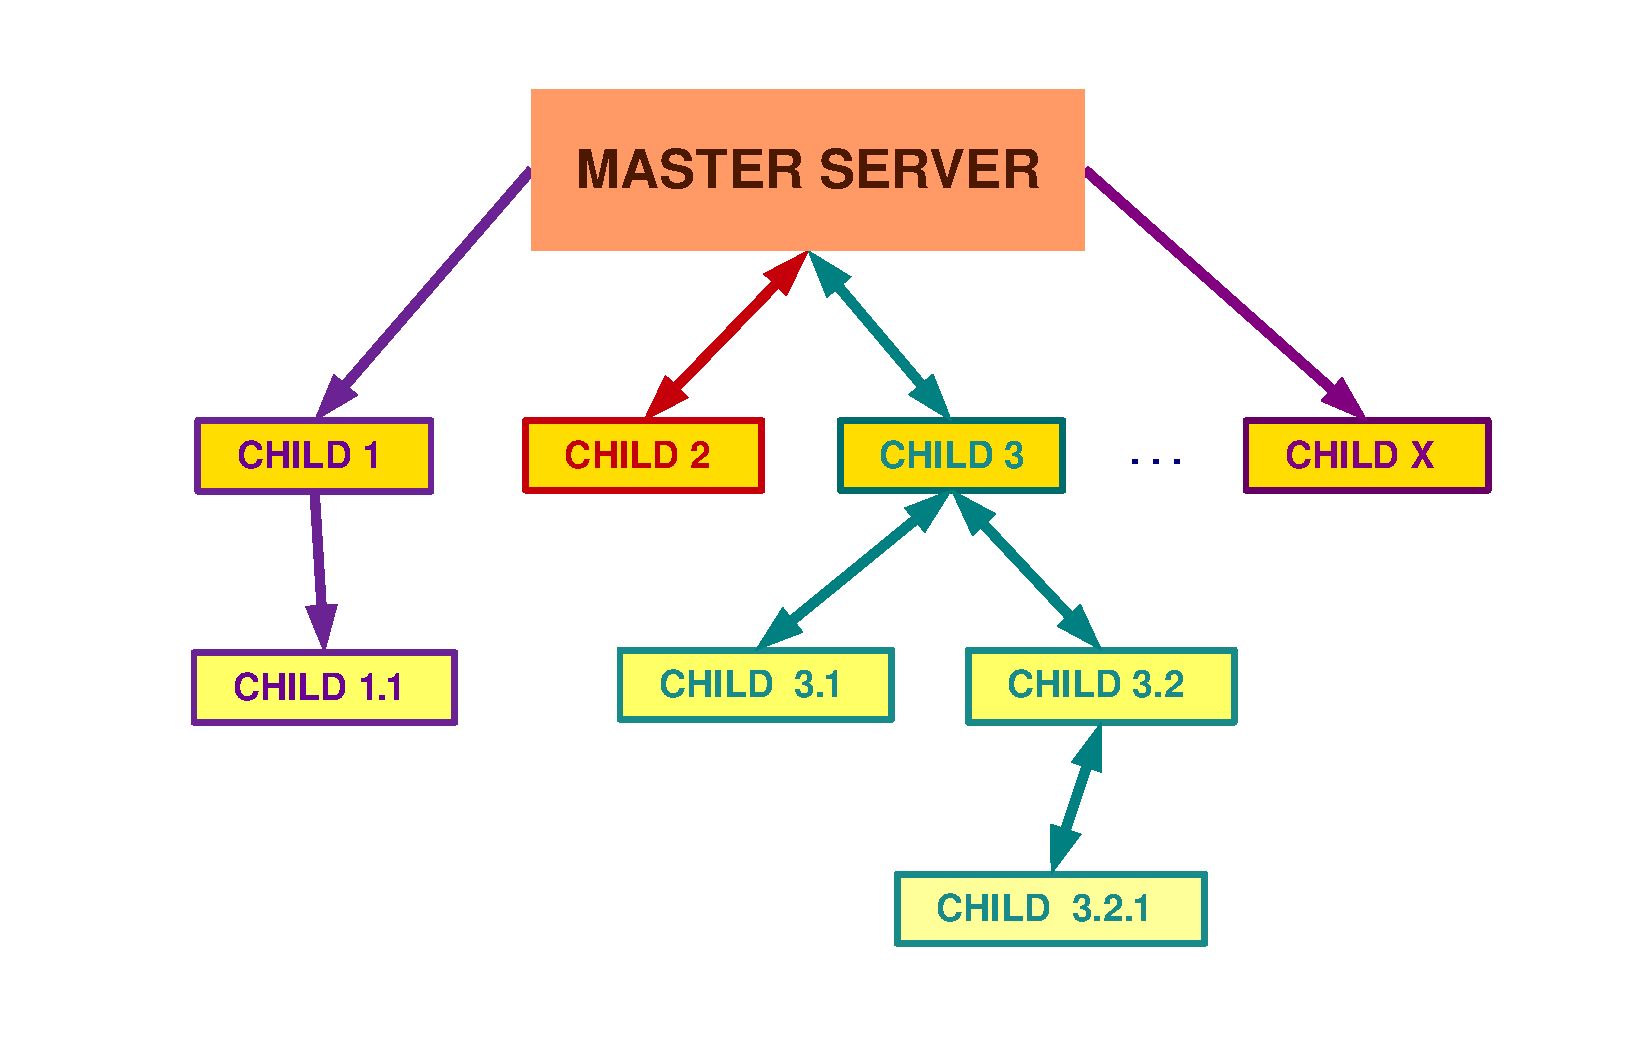
\includegraphics[width=\textwidth]{MMDlib_SC_hierarchy.pdf} 

  {\Huge\bf Multi-Model-Driver (MMD) \\Version 2.0 Library Manual}\\[12mm]

  {\huge\bf Astrid Kerkweg$^{1,3}$ \& Patrick J\"ockel$^2$ }\\[5mm]

  \large
  $^1$ Institute for Atmospheric Physics\\
  University of Mainz, 55099 Mainz, Germany\\
  $^2$ Deutsches Zentrum f\"ur Luft-und Raumfahrt (DLR),\\
   Institut f\"ur Physik der Atmosph\"are, \\
    Oberpfaffenhofen, D-82234 We\ss ling, Germany \\
  \url{patrick.joeckel@dlr.de}\\
  $^3$ Meteorological Institute\\
  University of Bonn, 53121 Bonn, Germany\\
  \url{kerkweg@uni-bonn.de}\\

\end{center}

\vfill

{\large This manual is available as electronic supplement of our article
  ``The on-line coupled atmospheric chemistry model system MECO(n)
  – Part 5: Expanding the Multi-Model-Driver (MMD v2.0) for 2-way data
  exchange including data interpolation via GRID (v1.0) '' 
  in Geosci.\ Model Dev.\ 
  (2018), available at: \url{http://www.geosci-model-dev.net}}

\begin{center}
%  Date: \thedate
  Date: \today
\end{center}

\newpage%\twocolumn

\sloppy

\tableofcontents
\clearpage


\section{Introduction}
This is the documentation of the second release of the Multi-Model-Driver (MMD)
library. The first MMD version was written following a Client-Server
approach, where the Server (driving model) provides data  
to a Client model. The most prominent
application is a global model driving a regional model. 
For the data exchange the sending and the receiving side must be distinguished.
Therefore the model instance sending the information was called ``server'' and
 the model receiving data was named ``client''.
The current version of the Library is extended to allow data exchange in both
directions. Here, the application in mind is the two-way coupling of
two models. In order to keep the naming convention of the first
version, one model instance (mostly the model determining the overall
time control) 
is still called the ``server'' or ``parent'', while the other model is
called the ``client'' or ``child''. 
Furthermore the model providing / sending data is called {\it sending
model}\footnote{ 
Throughout the manual some words are written in italics. Their meaning
is explained in the appendix of the manual.} (or
short the {\it Sender}) and the model receiving the data the {\it receiving
model} (or short the {\it Receiver}). 
The other model instance in a corresponding pair of instances  is
further denoted as {\it remote model}, i.e.,  
the {\it remote model} of the server / parent is the client / child
model and vice versa. Note: The terms ``model'', ``model instance''
and ``instance'' do not mean exactly the same thing. A ``model'' is
the model itself (e.g., for the MECO(n) system these are COSMO/MESSy
or EMAC). In an MMD coupled system different instances of these
models are run concurrently. Thus a ``model instance'' or ``instance''
is one realisation of the model configuration within the coupled setup.
However, as it is intuitively clear whether a ``model'' or an
``instance'' is addressed, we will use these terms synonymously.


 MMD consists of two parts:
\begin{itemize}
\item the Multi-Model-Driver (MMD) library provides all routines necessary for 
the data exchange between executables of basemodels, and
\item the submodel MMD2WAY organises the data sending to and receiving 
from the respective remote model and the further processing of the data.
\end{itemize}
The MMD library manages the communication between the remote models.
The submodel MMD2WAY controls the data exchange via namelists. It is
split into two sub-submodels MMD2WAY\_PARENT and
MMD2WAY\_CHILD\footnote{Remark for those readers familiar with the first
version of MMD: MMD2WAY\_PARENT and  MMD2WAY\_CHILD are, with respect
to the 1-way coupling, identical to MMDSERV and MMDCLNT, respectively.}.
The sub-submodel MMD2WAY\_PARENT comprises the data management
required for a parent submodel, while MMD2WAY\_CHILD deals with the
data management required by a child model.

In this manual we focus on the technical structure and functionality of the MMD 
library. A description of MMD2WAY is provided within the 
``MMD user manual'', available in the same electronic supplement as this manual.
 The MMD library manages the data exchange very efficiently, as the field 
exchange during the time integration is implemented as point-to-point, 
single-sided, non-blocking MPI\footnote{Message Passing Interface} communication.

The MMD library is implemented in a way that an arbitrary number of
model instances can be run concurrently within the same MPI environment. 
Each instance can be parent for an arbitrary number (including zero) of other
instances and is child of exactly one instance. The only exception is the
 global or ``coarsest'' instance of the setup. This one drives all the
 other instances 
(directly or indirectly via other child models), but is not child model of
any other model itself. This model is called {\it master parent} or
{\it patriarch}. 
The figure on the front page of the manual gives an example for a possible
 model cascade.
Here, the {\it patriarch} ``serves'' four child models (CHILD 1,2,3
and X). Two of these child models (CHILD 2 and 3) send data back to their
parent, which is indicated by the double-ended arrows.
CHILD 1 and 3 are parent for other child models as well. CHILD 1 has one child 
model (CHILD 1.1) and CHILD 3 serves two child models (CHILD 3.1 and CHILD
3.2), which both send
back to CHILD 3. CHILD 3.2 is  parent model for CHILD 3.2.1
and receives data from it.
The child models of a parent model are completely independent of each other. 

The only restrictions for such a model cascade are those usually valid for the 
nesting of limited-area models into coarser models. 
For instance, each child model domain, including an additional
boundary required for interpolations from the coarser to the finer
grid, has to be embedded entirely into the parent domain.
These requirements become more complex, if the same data are sent back
from different child models to the same parent model. 
There is no interference as long as the child model domains do not
overlap. If they do, the data from the childrens are applied in the
order of the child instances.
However, if different data are exchanged the overlap is technically no
problem.
Anyhow, it is left to the user to construct a scientifically meaningful
setup. The library ``only'' provides the infrastructure to exchange the data.

The MMD library is mainly written in Fortran95 and partly in C. On the
 one hanf, C is
 required, as the data exchange during the time loop is 
implemented as single-sided communication.
 The buffer for the data  exchange is allocated by the MPI 
subroutine \verb|MPI_alloc_mem| which works properly only in C, as it hands
 back the memory address of the buffer, which cannot be used in Fortran95.
On the other hand the library must be able to handle Fortran95 
{\footnotesize POINTER}s which  -- in contrast to C {\footnotesize POINTER}s -- 
do not have to be consecutive in memory. 

The MMD library comprises mainly parent and child model specific routines
organised in modules USEd by the MMD2WAY submodel,
and it contains routines USEd by the parent and child basemodels 
directly.
The names of the modules and the subroutines or functions indicate, whether 
the language is C or Fortran95. C files or functions are prefixed with 
\verb|'mmdc_'|, while Fortran95 files or routines begin with \verb|'mmd_'|. 
 Figure \ref{fig:MMD-files} illustrates the dependencies
 of the MMD library modules and their internal hierarchy.
\begin{figure*}
\begin{center} 
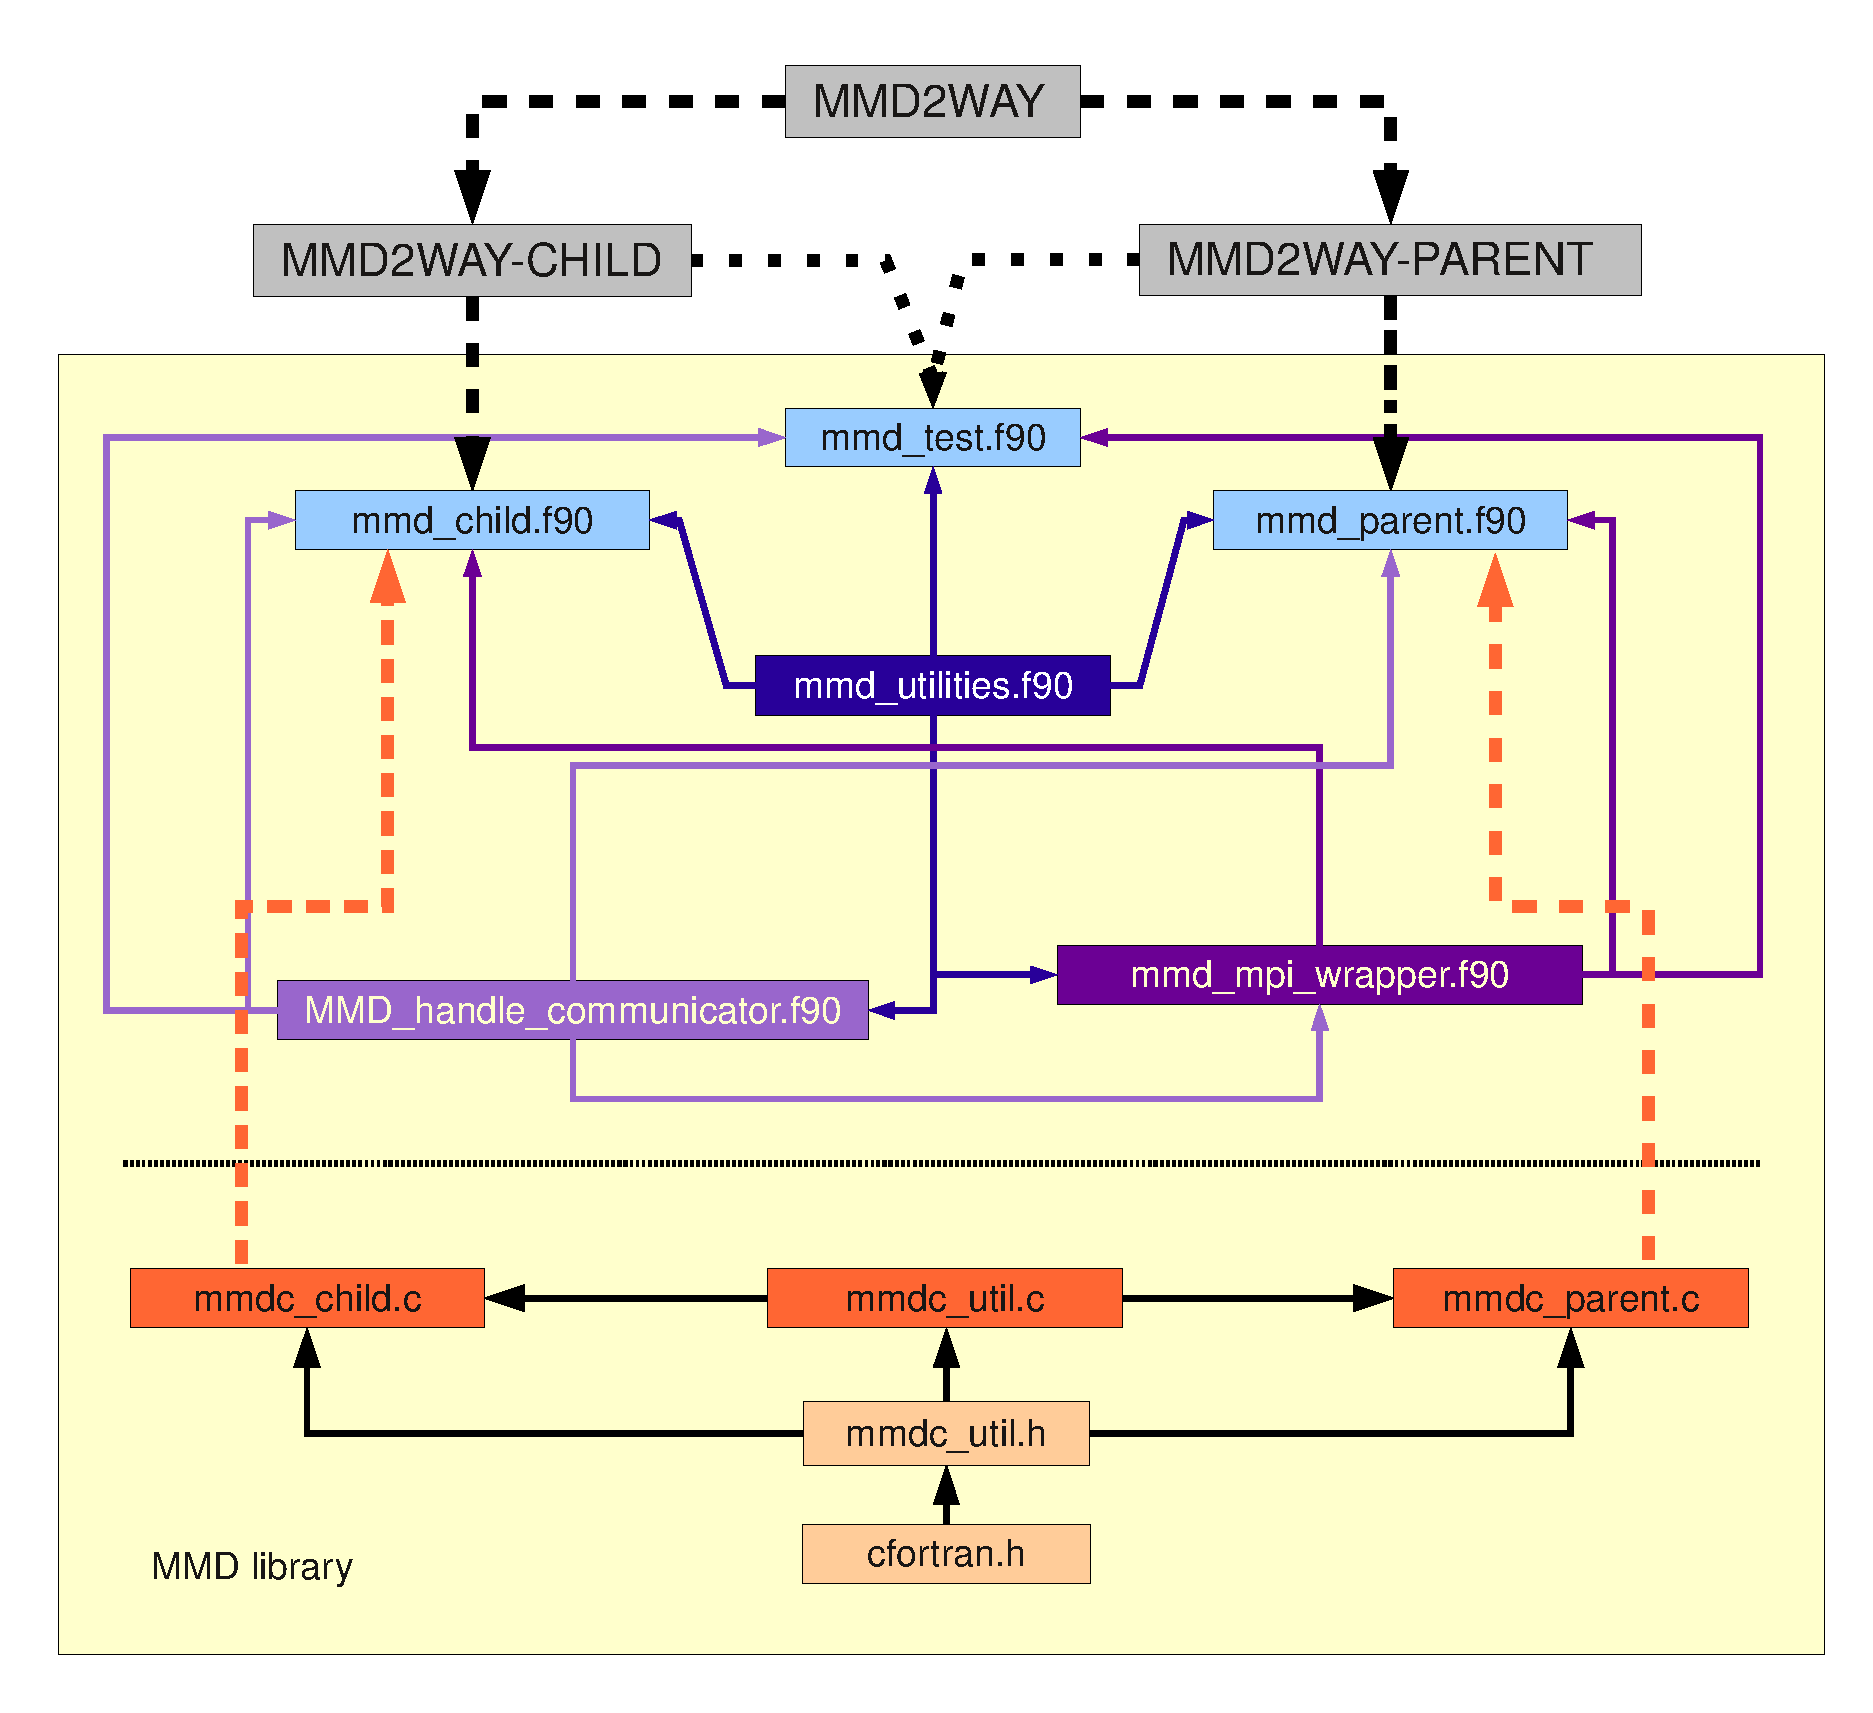
\includegraphics[width=\textwidth]{MMDlib_files.pdf} 
\end{center} 
\caption{Hierarchy of the MMD module files. Bluish colours indicate modules 
written in Fortran95, reddish colours denote C files. Arrows point in the
direction of USagE, e.g., {\tt mmd\_utilities.f90} is used by all other 
Fortran95 modules.} 
\label{fig:MMD-files} 
\end{figure*}
The arrows point into the direction of USagE. The Fortran95 part of the 
library (bluish colours in Fig.\ \ref{fig:MMD-files}) comprises six modules:
\begin{itemize}
\item \verb|mmd_child.f90|, 
\verb|mmd_parent.f90| and \verb|mmd_test.f90| are directly used by
the child and parent submodels (MMD2WAY\_CHILD and MMD2WAY\_PARENT,
 respectively). 

 All three module files in turn USE the three modules 
\verb|mmd_mpi_wrapper.f90|, \verb|mmd_handle_communicator.f90|  and 
\verb|mmd_utilities.f90|. 
\item \verb|mmd_mpi_wrapper.f90| supplies high level 
interface routines, which simplify the communication between parent and child
model 
and offer the possibility for alternative communication implementations without
 the need for changing the interfaces.
\item \verb|mmd_handle_communicator.f90|
contains the subroutines for the MPI-communicator definitions in the coupled
system. 
\item \verb|mmd_utilities.f90|  hosts the 
definition of the Fortran95 structures storing the information about the
MPI-communicators and the Fortran95 structure keeping the
information and data of the {\it exchange fields}.
\end{itemize}

The C part of the library (reddish colours in
Fig.\ \ref{fig:MMD-files}) contains five files:
\begin{itemize}
\item  \verb|mmdc_child.c| and \verb|mmdc_parent.c| contain the child model and 
parent model specific functions for the data exchange management. 
\item \verb|mmdc_util.c| supplies the declaration 
of the data structures. 
\item All three C modules access the header file 
\verb|mmdc_utils.h|, which itself uses the header
file \verb|cfortran.h| for C to Fortran95 binding. 
\end{itemize}
For the sake of a better readability only the file names without the language 
suffixes (\verb|.f90| or \verb|.c|) are used in the remaining text.

The next section provides an overview of the MMD library by describing the 
typical call sequence of the library routines. More detailed explanations 
 are provided in  Sect.\ \ref{sec:MMDdescript}. Subsect. 
\ref{sec:MMD-Fortran} describes the Fortran95 routines, Subsect.\ 
\ref{sec:MMD-C} the C functions of the MMD library. Last but not least,
 Subsect.\ \ref{sec:example} provides an example to illustrate the data 
exchange. 

%**************************************************************************
\section{The call sequence of the MMD library\label{sec:workflow}}

This section illustrates the interaction and the call sequence of the 
MMD library subroutines and functions, which are described in detail in Sect.\
\ref{sec:MMDdescript}. 
Fig.\ \ref{fig:MMD-workflow} shows the call tree.
 The yellow area indicates the initialisation
 phase of a simulation with MMD coupled 
models. The cyan part highlights those routines called during the 
 integration phase, and the lilac part denotes to the finalisation phase. 
The left hand side lists the routines called by the child model, the
 right hand side those called by the parent model.
Subroutines on the same level are called concurrently from the corresponding 
entry points in the child and parent model. Note that the names of the
 child model 
 specific 
 routines always start with ``\verb|MMD_C_|'', whereas the names of the parent 
specific routines begin with ``\verb|MMD_P_|''.  The names of the routines for 
 checking the consistency of the setup of the coupled models start with 
``\verb|MMD_testC_|" or ``\verb|MMD_testP_|" depending on the calling model, 
child or parent, respectively.

\begin{figure}
\begin{center} 
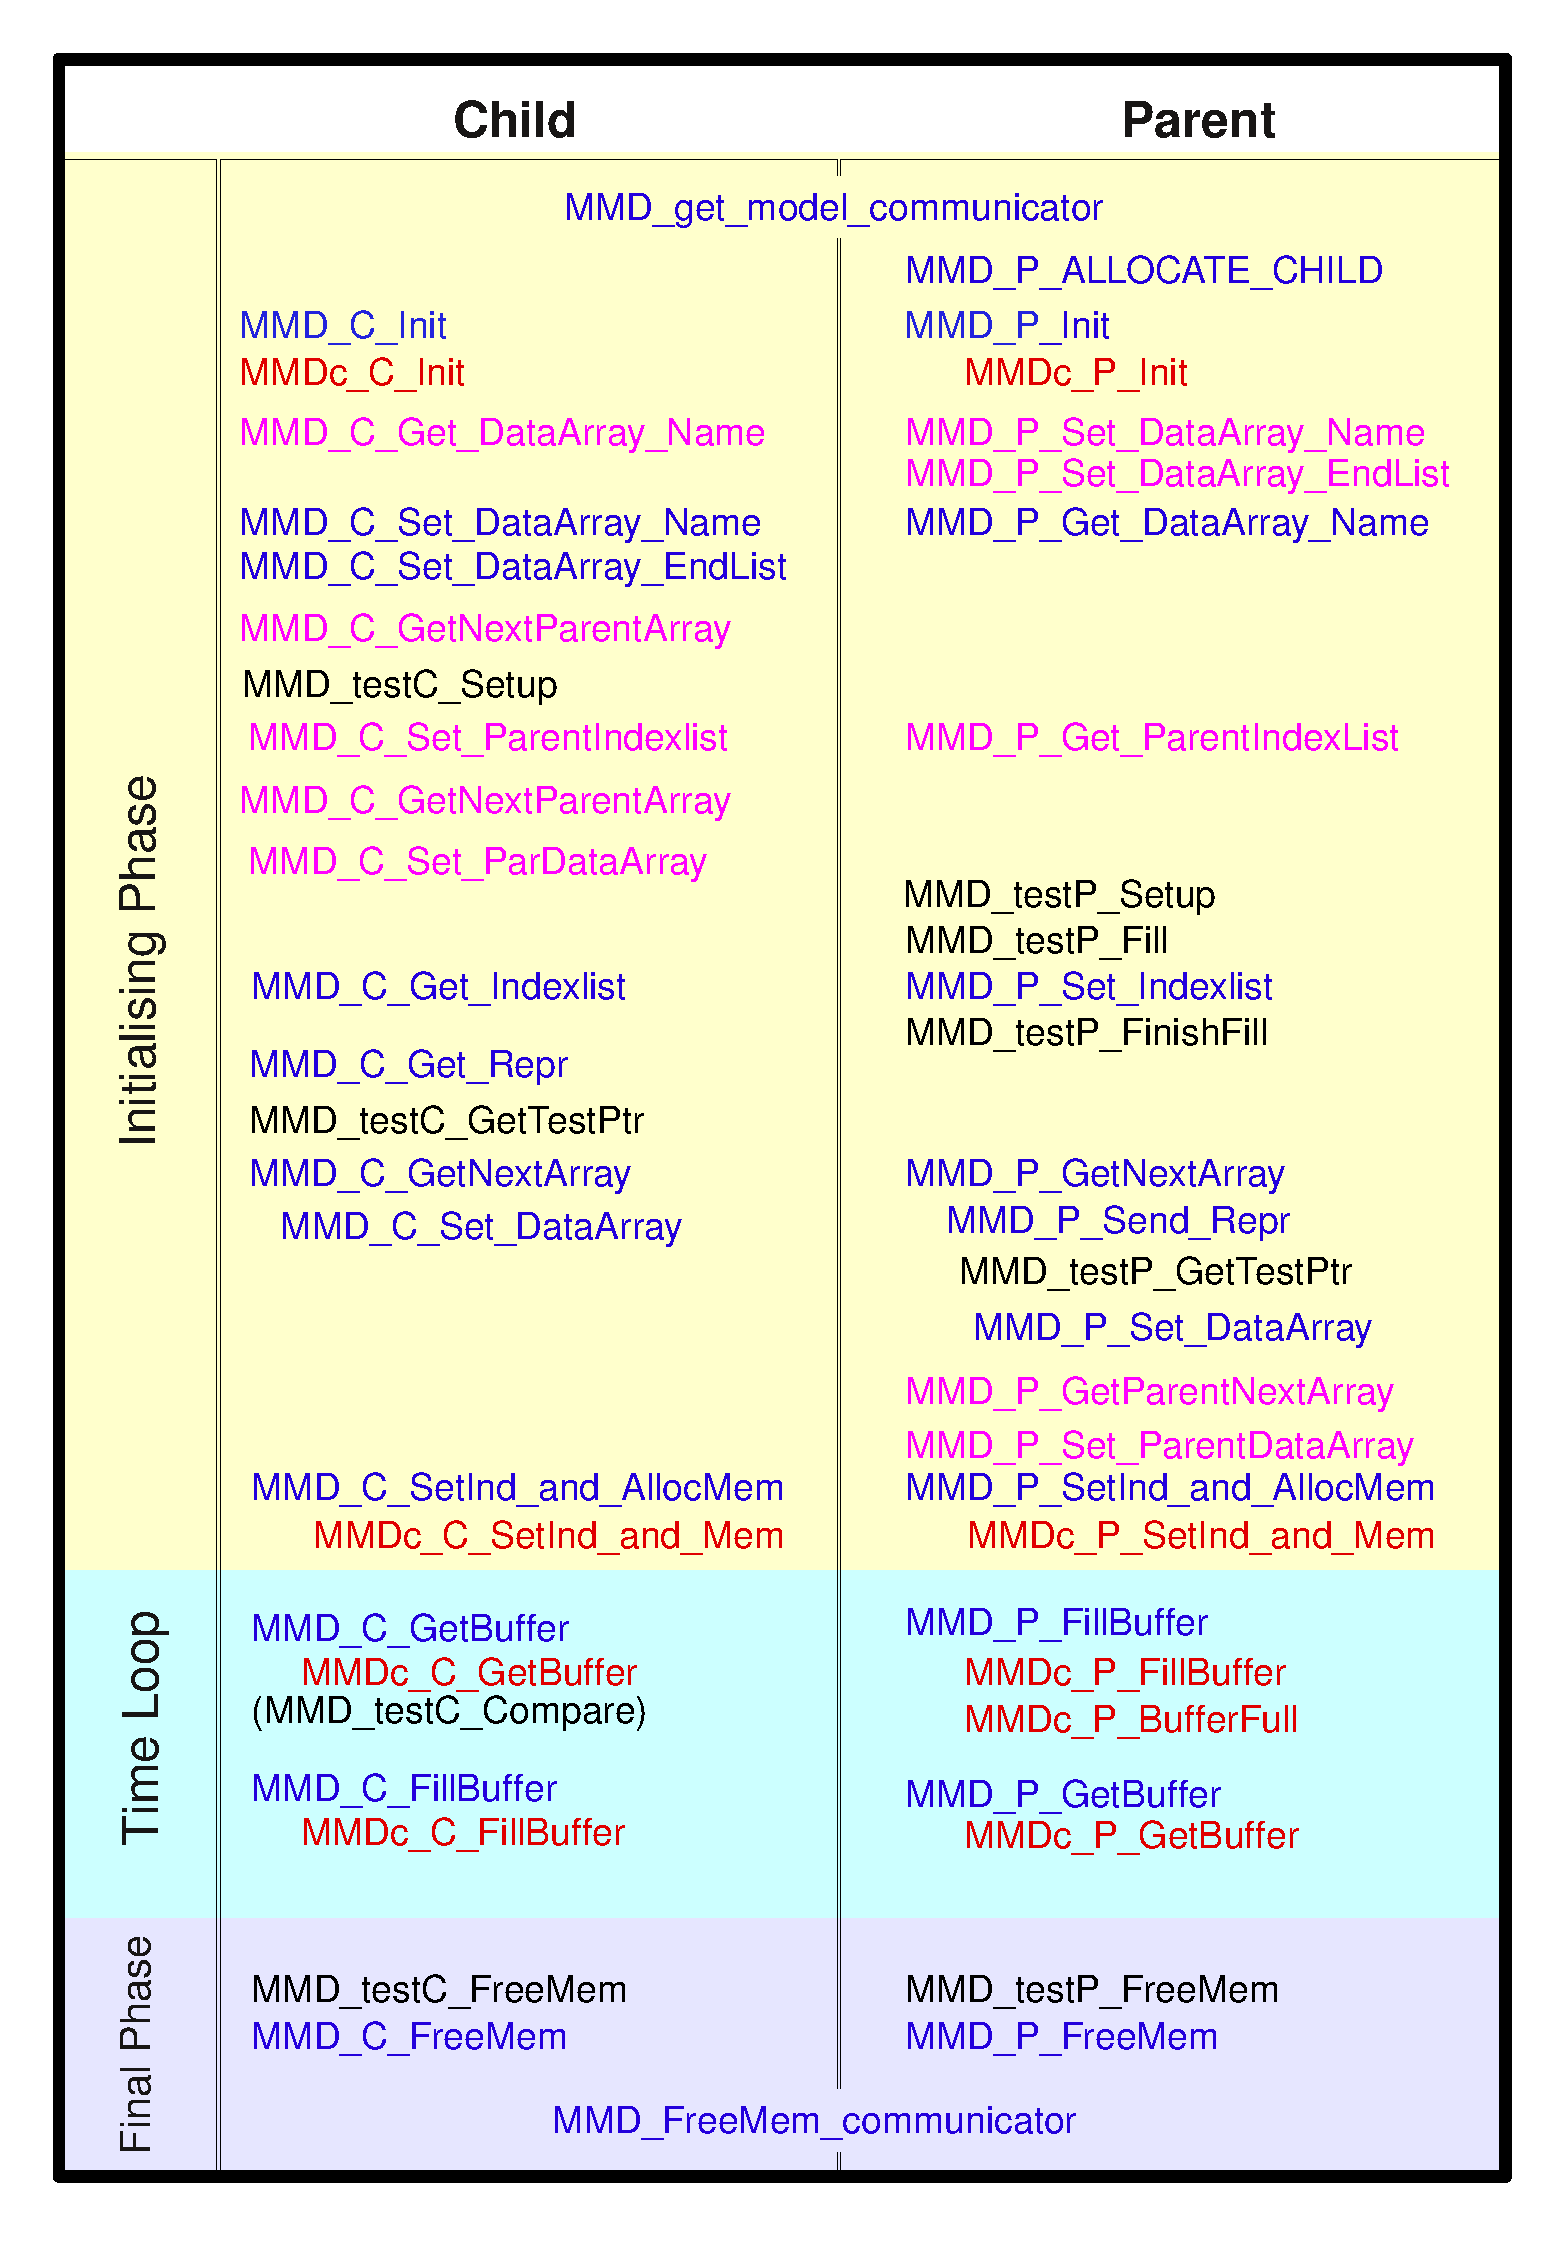
\includegraphics[height=0.86\textheight]{MMDlib_work_flow.pdf} 
\end{center} 
\caption{Systematisation of the MMD library: blue are the names of the
 child and parent model specific Fortran95 routines of the MMD
 library, red are the C functions, 
pink are the subroutines added for the 2-way coupling, whereas the
black colour indicates the routines required for the test setup  
(written in Fortran95).} 
\label{fig:MMD-workflow} 
\end{figure} 
\subsection{The initialisation phase} \label{ssec:initialp}
At the very beginning, the MPI-communicators of the different models/parallel
processes are determined. In addition to the ``global'' MPI-communicator 
\verb|MPI_comm_world| containing all process entities\footnote{Here equivalent
to MPI tasks.} (PEs), a group communicator is set up for each model. 
This is achieved by the subroutine \verb|MMD_get_model_communicator|. 
It is called during the MPI setup procedure of all models. 
Within this subroutine the namelist file \verb|MMD_layout.nml|, which 
contains all information defining the coupling layout of 
all instances for the current simulation, is read by the process (PE) with
\verb|m_world_rank = 0| and broadcasted to all other processes.
 Afterwards, the communicators are defined based on the namelist information,
i.e., a group of PEs is associated to each model instance and the corresponding
group communicator is defined.
The subroutines \verb|MMD_get_model_communicator| and  
\verb|MMD_FreeMem_Communicator| are the only subroutines, which are called
 directly from the basemodels. All other routines are called from
 the MESSy submodel MMD2WAY carrying out the coupling.

\begin{itemize}
\item
In the parent model specific subroutine \verb|MMD_P_Allocate_Child| the
 structure \verb|Child|, which components contain all required
information about the child models and about the data requested by
 the respective child model, is allocated
 to the actual number of child models of each individual parent models. 
For instance, in the example on the front page the {\it patriarch} requires
 space for 4 child models, whereas CHILD 1 provides data to only one
 child model. 
 In case of 2-way coupling, additionally the structure \verb|Parent|
 is allocated also to the number of child models. The components of this
 structure hold all information required for sending back data from the
 child models. 
 Additionally, arrays for the buffer length of the exchange data (\verb|ChldBL|
 and \verb|PArBL|) are allocated to the number of child models.
\item
In the subroutines \verb|MMD_P_Init| and \verb|MMD_C_Init| the MMD 
internal structure components containing the information about the
{\it remote model(s)} are 
allocated to the correct size according to the coupling
layout. Subsequently, the structure components are preset with
default values. 

Additionally, the setup routines for the C-core of MMD, \verb|MMDc_C_Init|
and \verb|MMDc_P_Init|, 
are called. Within these routines the communicators for the communication on
the C language level are constructed, and the information about the size (number
 of processes occupied by the {\it remote model}) is handed back to the 
Fortran95 part of the library.

\item
As a first step on the way to the data exchange between the models,
the parent and the child models 
provide lists of parent and child model {\it channel} and {\it channel object}
 names of the required data arrays and the corresponding {\it respresentation}
to the MMD library by calling the
subroutines \verb|MMD_P_Set_ParDataArray_Name|
and \verb|MMD_C_Set_DataArray_Name|, respectively.

Within the library routine \verb|MMD_P_Set_ParDataArray_Name| the {\it
channel} and {\it channel object} names of 
the fields required by the parent model are  
stored within the structure variable \verb|Parent|, which is of
TYPE \verb|ExchDataDef|(see Sect.\ \ref{sec:mmd_util}). \verb|Parent|
contains  the overall coupling information for the receiving parent model
part of the library. 
Additionally, this subroutines broadcasts the respective child model {\it
channel} and {\it channel object} names and their {\it
representation}s to the child model.  On the child model side the data is
received and processed within the
 subroutine \verb|MMD_C_Get_ParDataArray_Name|. Here, the 
{\it channel} and {\it channel object} names of the field sent
from the child to the parent model and their {\it representation}s
are stored in the structure variable \verb|Parent|, which is also of
TYPE \verb|ExchDataDef|.  
These information will be accessed later on using the functions
 \verb|MMD_P_GetNextParArray| and \verb|MMD_C_GetNextParArray|
 on parent and child model side, respectively.  

Subsequently, within the library
routine \verb|MMD_C_Set_DataArray_Name|, the {\it channel} and {\it
channel object} names of the fields required by the child model are  
stored within the structure \verb|Me|, which is of TYPE \verb|ExchDataDef|
and contains the overall coupling information required by the
receiving child model part of the library.
Additionally, within this subroutine the parent model {\it channel} and
 {\it channel object} names and their {\it representation}s 
are sent to the parent model. On the parent side the data is received
 and processed within the
 subroutine \verb|MMD_P_Get_DataArray_Name|. Here, the 
{\it channel} and {\it channel object} names of the parent model {\it exchange
fields} 
 and their {\it representation}s are stored in the information structure 
(\verb|Child|) for the respective child model. 
These information will be accessed later on, with the use of the functions
 \verb|MMD_P_GetNextArray| and \verb|MMD_C_GetNextArray| on parent and
 child model side, respectively.  

The subroutines \verb|MMD_P_Set_ParDataArray_Name|
and \verb|MMD_C_Set_DataArray_Name| are called for each {\it
channel} and {\it channel object} name pair independently. The calls to
the subroutines \verb|MMD_P_Set_ParDataArray_EndList|
and \verb|MMD_C_Set_DataArray_EndList|,respectively, indicate that the list
is complete.

\item
Additional preparations are performed before the data exchange can take place:
\begin{itemize}
\item First, the information is required, which local model PE exchanges which 
parts of its horizontal grid (including the indices in the respective
 local grid) with which remote model PE for both data exchange
 directions independently.
Hereafter, this information is refered to as ``\verb|index_list|''. It is
 provided by the MESSy submodel MMD2WAY to the MMD library as parameter to the 
subroutines \verb|MMD_P_Set_Indexlist|
 and \verb|MMD_C_Set_ParIndexlist| for 1-way and backward coupling,
 respectively. 
 Within the subroutine \verb|MMD_P_Set_Indexlist| the information for the
 data exchange from the parent to the child model is processed (see
 Sect.\ \ref{sec:mmd-parent}). Similarly,
 in \verb|MMD_C_Set_ParIndexlist| processes the information for the exchange
 between child and parent model.
 In these subroutines, the indexlists are evaluated and sent to the
 respective remote model. The remote model receives and processes 
this list within the subroutines \verb|MMD_C_Get_Indexlist|
 and \verb|MMD_P_Get_ParIndexlist|, respectively. 
For further details see the description of the subroutines 
\verb|MMD_P_Set_Indexlist| in Sect.\ \ref{sec:mmd-parent}
 and \verb|MMD_C_Set_ParIndexlist| in Sect.\ \ref{sec:mmd-child}. 
\item Second, a test is initiated for checking the data exchange from
the parent to the child model. All subroutines with names starting
with \verb|'MMD_test'| contribute to this consistency check. 
\item Third, the connection between the {\it channel} and 
{\it channel object} names to the respective Fortran95-{\footnotesize
POINTER}s need to be established:
\begin{itemize}
\item Data exchange from parent to child model:
\begin{itemize}

\item On the parent model side, the list 
of the names of the {\it exchange fields} established by the subroutine 
\verb|MMD_P_Get_DataArray_Name| is provided to MMD2WAY\_PARENT by the
subroutine \verb|MMD_P_GetNextArray|. For each of the required fields 
the MESSy submodel MMD2WAY\_PARENT provides a 4D-{\footnotesize POINTER} to the 
memory of the respective {\it exchange field}
as parameter to the subroutine \verb|MMD_P_Set_DataArray|. Additionally,
 the local {\it dimensions} and the {\it axis string} related to this particular
 field are parameter to this subroutine. This information is stored in the 
respective structure components and analysed: the {\it dimensions} determine the
 memory size (buffer length) required for the data exchange.
The {\it axis string} is used later during the integration to re-arrange the data 
(before the actual data exchange) into a 1D-array. The sum over all individual 
buffer sizes is the buffer length required for the data exchange of all data 
fields from each individual parent PE to all child model PEs. This number is
used to  
actually allocate the required memory with the C function 
\verb|MMDc_P_SetInd_and_Mem|, which is called via the Fortran95 subroutine 
\verb|MMD_P_SetInd_and_AllocMem|. 
\item For the child model the provision of the data {\footnotesize POINTER}
via the  
subroutines and functions \verb|MMD_C_Get_DataArray_Name|, 
\verb|MMD_C_GetNextArray| and  \verb|MMD_C_Set_DataArray| works similarly.
The {\it dimension} and {\it axis string} information are used during the 
integration phase to re-order the 1D-array received from the parent into the
4D data arrays as requested by the child model.
\end{itemize}

\item Data exchange from child to parent model:
\begin{itemize}
\item On the child model side, the list 
of the names of the {\it exchange fields} established by the subroutine 
\verb|MMD_C_Get_ParDataArray_Name| is provided to MMD2WAY\_CHILD by the
subroutine \verb|MMD_C_GetNextParArray|. For each of the required fields 
the MESSy submodel MMD2WAY\_CHILD provides a 4D-{\footnotesize POINTER} to the 
memory of the respective {\it exchange field}
as parameter to the subroutine \verb|MMD_C_Set_ParDataArray|. Additionally,
 the local {\it dimensions} and the {\it axis string} related to this particular
 field are parameter to this subroutine. This information is stored in the 
respective structure components and analysed: the {\it dimensions} determine the
 memory size (buffer length) required for the data exchange.
The {\it axis string} is used later during the integration to
re-arrange the data  
(before the actual data exchange) into a 1D-array. The sum over all individual 
buffer sizes is the buffer length required for the data exchange of all data 
fields from each individual Child PE to all Parent PEs. This number is used to 
actually allocate the required memory with the C function 
\verb|MMDc_C_SetInd_and_Mem|, which is called via the Fortran95 subroutine 
\verb|MMD_C_SetInd_and_AllocMem|. 
\item For the parent model the provision of the data {\footnotesize POINTER}
via the  
subroutines and functions \verb|MMD_P_Get_DataParArray_Name|, 
\verb|MMD_P_GetNextParArray| and  \verb|MMD_P_Set_ParDataArray|
works similarly. 
The {\it dimension} and {\it axis string} information is used during the 
integration phase to re-order the 1D-array received from the child model into
the 4D data arrays as requested by the parent model.
\end{itemize}

\end{itemize}
\end{itemize}

\end{itemize}
At this point all preparations required for the data exchange are finished
and the actual data exchange starts.

\subsection{The time loop} \label{ssec:timeloop}
As the data exchange was fully prepared in the initialisation phase,
the buffers only need to be filled and read  within the time 
loop. Here, the order of MMD library routine calls is important to
avoid an MPI deadlock:
\begin{enumerate}
\item The parent model has to fill the buffer. This is done by the MMD library
subroutines \verb|MMD_P_FillBuffer| and \verb|MMDc_P_FillBuffer|
(see Sect.\ \ref{sec:mmd-parent}).
After the buffer is filled, it is made accessible for the child model
by setting a barrier indicating that the buffer is filled. 
\item Afterwards this buffer can be read by the child model.
 Within the subroutines  
\verb|MMD_C_GetBuffer| and \verb|MMDc_C_GetBuffer| the (1D-)buffers
are read and  
re-arranged to the 4D-data fields according to the corresponding {\it axis 
string} and the local {\it dimensions}. 
If only 1-way coupling is required, again a barrier is set to indicate
to the parent that the buffer was read and can be filled again, i.e.,
the cycle starts again with 1. (3.+4. are omitted for 1-way coupling).
\item After the buffer is read by the child model, it can be filled with the
child model data coupled back to the parent model. This is performed by the
subroutines \verb|MMD_C_FillBuffer| and \verb|MMDc_C_FillBuffer|. At
the end of this subroutine a barrier is set to indicate that the
buffer is filled by the child model and ready for being read by the parent model. 
\item In the last step of the cycle in the
subroutines \verb|MMD_P_GetBuffer| and \verb|MMDc_P_GetBuffer| 
the data provided by the child model are read from the parent and
re-arranged into the requested 4D-data format according to the
corresponding {\it axis string} and the local {\it dimensions}. After
the reading is finished, the cycle starts again.
\end{enumerate}

To detect errors in the data exchange the
subroutine \verb|MMD_testC_Compare| is called after the first data exchange.
The transferred test arrays containing the geographical longitudes and
latitudes are compared to the original arrays of the child model. 
If they do not match, the simulation is terminated with an error message.

\subsection{The finalisation phase} \label{ssec:finalp}
At the end of the simulation the memory allocated during the initialisation must
be deallocated. The test arrays are deallocated within the subroutines 
\verb|MMD_testC_FreeMem| and \verb|MMD_testS_FreeMem|, respectively.
 The memory allocated
for the MMD library data structures is released in \verb|MMD_C_FreeMem| and 
\verb|MMD_P_FreeMem| for child and parent model, respectively.
Last but not least, the memory allocated by the subroutine 
\verb|MMD_get_model_communicator| is released within the subroutine 
\verb|MMD_FreeMem_Communicator|.

%**************************************************************************
%**************************************************************************
\section{Detailed library description}\label{sec:MMDdescript}
In this section the definitions and routines of the MMD library are
described in detail. The Fortran95 and the C part are explained in individual 
subsections. Each of the subsections is split into subsubsections dedicated to 
one (module) file each. 
Each subsubsection contains the interface declarations of the routines 
of the respective module. Their content and usage are described subsequently.
The section is closed with an example illustrating the definitions of the
index and length variables used in the C and the Fortran95 part.
%**************************************************************************
\subsection{The Fortran95 part of the MMD library}\label{sec:MMD-Fortran}
The Fortran95 part of the library is the interface between the coupled models
(more precisely between the coupling subsubmodels MMD2WAY\_CHILD and
MMD2WAY\_PARENT) 
and the C routines providing the infrastructure for the data exchange during the
 integration. The library modules are described in the order of their 
dependencies. As the three main interface modules \verb|mmd_child.f90|, 
\verb|mmd_parent.f90| and \verb|mmd_test.f90| are completely
independent of each other, they are described in an arbitrary order.

\subsubsection{\tt mmd\_utilities}\label{sec:mmd_util}

\verb|mmd_utilities| is used by all other Fortran95 modules. It provides the 
definition of the data structures containing all information about
the model system setup, the communicators, about the structure of the data, 
 the \verb|index_list| for the data exchange between two models and
 the definition of some {\footnotesize PARAMETER}s controlling the coupling
 procedure:
\begin{verbatim}
! ****************************************************************
! from messy_main_constants_mem.f90
INTEGER, PARAMETER, PUBLIC  :: MMD_DP = SELECTED_REAL_KIND(12,307)
INTEGER, PARAMETER, PUBLIC  :: MMD_I8 = SELECTED_INT_KIND(14)

INTEGER, PARAMETER          :: DP=MMD_DP

! Length of Data Array Name 
INTEGER,PARAMETER, PUBLIC   :: STRLEN_CHANNEL = 23     
! Length of Data Array Name
INTEGER,PARAMETER           :: STRLEN_OBJECT  = 55     
INTEGER, PARAMETER, PUBLIC  :: STRLEN_MEDIUM  = 24
INTEGER,PARAMETER, PUBLIC   :: STRLEN_ULONG   = 256
! ****************************************************************

! ****************************************************************
! Definition PARAMETER
INTEGER,PARAMETER,PUBLIC :: MMD_ParentIsECHAM = 1
INTEGER,PARAMETER,PUBLIC :: MMD_ParentIsCOSMO = 2
! return status
INTEGER,PARAMETER,PUBLIC :: MMD_STATUS_OK    = 0
INTEGER,PARAMETER,PUBLIC :: MMD_DA_NAME_ERR  = 10

INTEGER,PARAMETER,PUBLIC :: MMD_MAX_MODEL    = 64
! ****************************************************************
\end{verbatim}


The first block defines the  {\footnotesize KIND PARAMETERs}
 and the string lengths required
within the library identically to the MESSy definitions. The second block 
consists of MMD internal settings.
In the specific application of the MMD library, the 
MESSy subsubmodel for the coupling on the child model side (MMD2WAY\_CHILD)
 requires 
 the information about the parent model type (spectral (gaussian grid) =
 ECHAM = gaussian grid or COSMO = lat-lon grid), as some parts of the
 interpolation/coupling procedure depend on the parent model type.
The {\footnotesize INTEGER PARAMETERs} \verb|MMD_ParentIsECHAM| and 
\verb|MMD_ParentIsCOSMO|
are used to indicate, whether the parent is ECHAM or COSMO. This list can be
expanded by newly introduced models.  \verb|MMD_STATUS_OK|
and \verb|MMD_DA_NAME_ERR| define some specific error values. 
\verb|MMD_MAX_MODEL| determines the number of model instances maximally
handled by MMD.  
If more than 64 model instances shall be run in parallel by MMD, this number needs to be 
increased within the code. 


The {\footnotesize TYPE} \verb|ExchDataDef| includes all information
required to associate the correct data, dimensions of data fields and
grid points to each other:
\begin{verbatim}
 TYPE ExchDataDef
    ! REMOTE MODEL ID
    INTEGER                            :: RMId       = 0
    ! NUMBER OF REMOTE MODEL PEs
    INTEGER                            :: inter_npes = 0   
    ! STRUCTURE FOR EACH PE
    TYPE(PeDef), DIMENSION(:), POINTER :: PEs
    ! INDEX LIST OF PARENT MODEL POINTS
    INTEGER,DIMENSION(:,:),ALLOCATABLE :: index_list_2d
    ! Number of Points in index_list
    INTEGER                            :: NrPoints 
    ! ARRAY INFORMATION STRUCTURE (SAME ON ALL PEs)
    TYPE(ArrayDef_list), POINTER       :: Ar         => NULL()
    TYPE(ArrayDef_list), POINTER       :: ArrayStart => NULL()
  END TYPE ExchDataDef
\end{verbatim}
This structure defines the setup of exactly one {\it remote
model}. Therefore the child model needs one scalar variable of the type
of these structures, whereas each parent needs an array dimensioned by
the number of child models. 

\verb|RMId| is the identification number (ID) of the {\it remote 
model} within the overall MMD setup. It is equal to the instance
 number, e.g.\ for the example given in Sect.\ \ref{sec:handle-comm}
 and Fig.\ \ref{fig:modeltree}, COSMO/MESSy 3.2 has 
 \verb|RMId=8|. The \verb|RMId| is only used by a parent model.

\verb|inter_npes| gives the number of processing entities (PEs) used by the 
{\it remote model}, i.e., for the child model the number of parent PEs is
stored, whereas for a parent model the number of child model PEs is required.

During the initialisation of MMD the structure component \verb|PEs| will be 
dimensioned with \verb|inter_npes| as the structure components of  
{\footnotesize TYPE} \verb|PeDef| get specific values for each PE of the 
{\it remote model}:
\begin{verbatim}
  TYPE PeDef
     INTEGER                             :: NrEle   ! Number of Elements 
     TYPE(xy_ind), POINTER, DIMENSION(:) :: locInd
  END TYPE PeDef
\end{verbatim}
 \verb|NrEle| is the number of elements 
exchanged with each individual {\it remote model} PE\footnote{Note: as the library is 
run in the parallel decomposition of the respective model, {\tt NrEle} and {\tt locInd} 
are different and specific for each PE.}:
 For a {\it receiving model} \verb|NrEle| is the number of grid points the
 {\it receiving model} PE gets from a specific {\it sending model} PE.
 For a {\it sending model} \verb|NrEle| is the number of grid 
points, which this {\it sending model} PE provides to a specific {\it
receiving model} PE. 
\verb|locInd| is dimensioned by \verb|NrEle| and contains the index pairs for
 each exchanged grid point in the particular local decomposed grid: 
\begin{verbatim}
  ! Pair of indices in horizontal plane
  TYPE xy_ind
     INTEGER :: i
     INTEGER :: j
  END TYPE xy_ind
\end{verbatim}
Thus, for the {\it receiving model}, \verb|locInd| contains the index
pairs of the local decomposed field as received from the {\it
sending model} (here after denoted {\it in-field}), whereas for the
{\it sending model} \verb|locInd| stores the indices in  
its own local decomposed model domain. 

Figure \ref{fig:MMD-NrEle} together with Table \ref{tab:ex1} illustrates these 
dependencies:
\begin{figure}
\begin{center} 
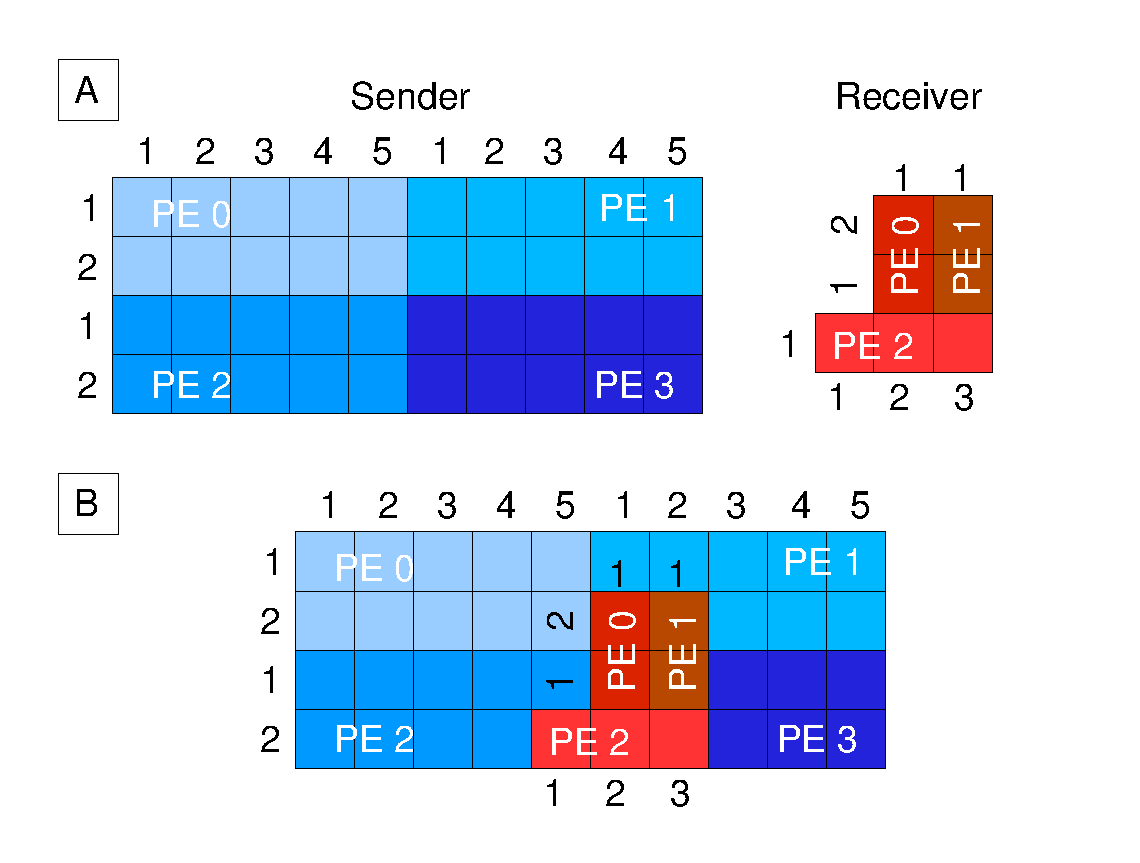
\includegraphics[width=0.85\textwidth]{MMDlib_NrEle.pdf} 
\end{center} 
\vspace*{-0.8cm}
\caption{Illustration of possible model domain overlaps and the definition
of the variable {\tt NrEle}. A detailed explanation is provided in the text.} 
\label{fig:MMD-NrEle} 
\end{figure} 

\begin{table}
\begin{center}
\begin{tabular}{|ccccc|} \hline
{\it Sender} & {\it Receiver} &       & (x,y)  & (x,y,) \\
 PE    & PE    & NrEle & index pairs & index pair \\
      &        &       &  {\it Sender} & {\it Receiver}\\  \hline
 0  &  0   &  0 & -&- \\
 0  &  1   &  0 & -&-  \\
 0  &  2   &  0 & -&-  \\
 1  &  0   &  1 & (1,2) & (2,1) \\
 1  &  1   &  1 & (2,2) & (2,1) \\
 1  &  2   &  0 & -&-  \\
 2  &  0   &  0 & -&-  \\
 2  &  1   &  0 & -&-  \\
 2  &  2   &  1 & (5,2) & (1,1)\\
 3  &  0   &  1 & (1,1) & (1,1)\\
 3  &  1   &  1 & (2,1) & (1,1)\\
 3  &  2   &  2 & (1,2)(2,2) & (2,1)(3,1)\\ \hline
\end{tabular}
\end{center}
\caption{Illustration of the data exchange between {\it sending} and
 {\it receiving model} PEs.
{\tt NrEle} is the number of elements exchanged, whereas the index
pairs show the identification of the grid points in the {\it sending
model} domain and the {\it in-field}  grid points in the {\it
receiving model} domain.}  
\label{tab:ex1}
\end{table}

Part A of Fig.\ \ref{fig:MMD-NrEle} shows two model domains. The left hand side
 illustrates the parallel domain decomposition of the {\it sending model} domain
 (blue). The {\it Sender} is run on  4 PEs. The decomposed model domains
 consist of 5x2 model grid boxes each. The model
 domain of the {\it receiving model} (red) was chosen to illustrate
 the grid association. The {\it receiving model}  is run on 3 PEs. The
 decomposed domains of PE 0 and PE 1 consist  
of 2x1 model grid boxes, that of PE 2 of 3x1 grid boxes. Part B of the figure 
shows the overlap of the {\it in-field} model domain of the {\it
 receiving model} with the {\it sending model}  domain. 
Table \ref{tab:ex1} gives the number (\verb|NrEle|) and the index pairs
 of exchanged elements for this example\footnote{Hereafter, individual 
horizontal elements are denoted using the syntax
 (i,j)$_{s~or~c,~PE~n}$. i and j are the index
 pair in the respective local parallel decomposed grid, s or r
 indicates {\it sending} or {\it receiving model}, respectively, and
 the respective PE of the {\it sending} or {\it receiving model} 
model is denoted by $PE~n$, with $n$ being the number of the PE.}:
 The {\it Sender} PE 3 sends the data of four grid boxes in total. One element is sent
 to {\it Receiver} PE 0 ((1,1)$_{s,PE3}$ $\rightarrow$
 (1,1)$_{r,PE0}$), one element (2,1)$_{s,PE3}$ is sent to {\it Receiver} PE
 1 and {\it Receiver} PE 2 gets two elements ((1,2)$_{s,PE3}$  and
 (2,2)$_{s,PE3}$). The {\it Receiver} PE 2  operates on three grid boxes and
 needs to get this number of elements. The {\it Receiver}
grid box (1,1)$_{r,PE2}$ on PE 2 is filled by {\it Sender} PE 2, which sends
 its grid box 
 (5,1)$_{s,PE2}$. The other two elements are provided by {\it Sender} PE 3:
 {\it Receiver} grid box
 (2,1)$_{r,PE2}$ gets the data from {\it Sender} grid box (1,2)$_{s,PE3}$
 and {\it Receiver} grid box (3,1)$_{r,PE2}$ gets the data of {\it Sender} grid
 box (2,2)$_{s,PE3}$. 

The information, which {\it Receiver} {\it in-field} grid box
corresponds to which {\it sending model} domain grid box is saved for
one Child-Parent pair in the structure 
 component \verb|index_list_2d|. \verb|index_list_2d| is only used
 during the  
initialisation phase and deallocated afterwards. Further details about 
\verb|index_list_2d| are provided in Sect. \ref{sec:mmd-parent} and Sect. \ref{sec:mmd-child}.


The structure component \verb|NrPoints| is only relevant on the {\it
 Sender} side of the library. 
It is the overall number of horizontal elements the current 
{\it Sender} PE has to send to all PEs of one {\it receiving model}.
 In the example this would be 0 for {\it Sender} PE 0, 2 for {\it
 Sender} PE 1, 1 for {\it Sender} PE 2 and 4 for {\it Sender} PE 3. 

Last but not least, the structure components \verb|Ar| and \verb|ArrayStart|
define a concatenated list, where  \verb|ArrayStart| points to the
first element of the list and \verb|Ar| to the actual one. The
{\footnotesize TYPE} 
 \verb|ArrayDef_list|
\begin{verbatim}
  TYPE ArrayDef_list
     TYPE(ArrayDef)               :: arrdef
     TYPE(ArrayDef_list), POINTER :: next
  END TYPE ArrayDef_list
\end{verbatim}
constructs a concatenated list of structure variables of {\footnotesize TYPE}
 \verb|ArrayDef|:

\begin{verbatim}
  TYPE ArrayDef
     CHARACTER(LEN=STRLEN_CHANNEL)          :: channel = '' ! Name of Channel  
     CHARACTER(LEN=STRLEN_OBJECT)           :: object  = '' ! Name of Object
     CHARACTER(LEN=STRLEN_MEDIUM)           :: repr    = '' ! Representation
                                                            !  of Object
     ! interpolation Method
     INTEGER                                :: interpM      
     LOGICAL                                :: l_sentunit 
     ! DATA POINTER
     REAL(DP), POINTER, DIMENSION(:,:,:,:)  :: p4 => NULL()

     CHARACTER(LEN=4)      :: dim_order = '    ' ! Order of dimensions
     INTEGER, DIMENSION(4) :: xyzn_dim  = 0      ! index of x,y,z,n dimension
     INTEGER, DIMENSION(4) :: dim       = 0      ! Size of Dimensions
     ! ArrLen and ArrIdx are different on each remote PE
     ! Dimension of Array moved   
     INTEGER, DIMENSION(:), POINTER :: ArrLen => NULL()
     ! Start Index of Array moved        
     INTEGER, DIMENSION(:), POINTER :: ArrIdx => NULL() 
  END TYPE ArrayDef
\end{verbatim}

This {\footnotesize TYPE} contains the description of one {\it exchange field}.
For the unambiguous identification of each {\it exchange field}, 
\verb|ArrayDef| contains the 
{\it channel} name, the {\it channel object} name and the {\it representation}
 name of the object. Additional information, on the interpolation method
 (\verb|interpM|) and, if the unit of the exchanged field needs to be
 transferred  (\verb|l_sentunit|), are structure components.

\verb|p4| is the {\footnotesize POINTER} to the respective memory,
 i.e., to the  
{\it in-field} on the {\it Receiver} side and to the variable on the
{\it Sender} side. 

The second block in the structure definition of \verb|ArrayDef| contains the
information about the dimensions and the order of the array:
\begin{itemize}
\item The {\footnotesize CHARACTER} string \verb|dim_order| indicates
the order of the {\it dimensions}
as string. The first and second horizontal axes are labelled with \verb|'X'| and
 \verb|'Y'|, respectively. The vertical axis is labelled with \verb|'Z'|. Each 
additional axis, e.g., number of tracer, number of aerosol modes, etc.,
is labelled by \verb|'N'|. If an axis is not used the label is  \verb|'-'|.
 \verb|dim_order| is a copy of the {\it axis string} defined in the CHANNEL 
submodel\footnote{The CHANNEL submodel is described in detail in 
\citeauthor{Joeckel10a}, GMD, \citeyear{Joeckel10a}}.
Table \ref{tab:orderdef} illustrates the definition of \verb|dim_order|.

%-------
\begin{table}
\begin{center}
\begin{tabular}{|lcccc|}\hline
description & representation & dim\_order & xyzn\_dim & dimension length \\ \hline
COSMO 3d & 'GP\_3D\_MID' & 'XYZ-' & (1,2,3,-1) & (ie,je,ke,-1) \\
ECHAM5 3d & 'GP\_3D\_MID' & 'XZY-' & (1,3,2,-1) & (nproma, ngpblks,nlev,-1) \\\hline
COSMO tracer & - & 'XYNZ' & (1,2,4,3) & (ie,je,ntrac,ke) \\
ECHAM5 tracer &  -  & 'XZNY' & (1,4,2,3) & (nproma,nlev,ntrac, ngpblks) \\\hline
\end{tabular}
\end{center}
\caption{Examples for the definition of the ArrayDef structure components 
{\tt dim\_order}, {\tt xyzn\_dim}, {\tt dim}.  The last column indicates the 
variable names of the respective dimension lengths in the respective model,
 i.e., {\tt ie} and {\tt nproma} are the 'X'-dimension lengths, 
 {\tt je} and {\tt ngpblks} the 'Y'-dimension lengths, 
{\tt ke} and {\tt nlev} the
 'Z' dimension lengths in the COSMO model and the ECHAM5 model, respectively. 
``-1'' denotes an unused rank.}
\label{tab:orderdef}
\end{table}
%-------

\item The {\footnotesize INTEGER} array \verb|xyzn_dim| provides the information at which rank 
which dimension can be found. The first entry indicates the rank of the 
\verb|'X'| dimension, the second that of the \verb|'Y'| dimension, the third
the \verb|'Z'| and the fourth the \verb|'N'| dimension. Unused dimensions are
labelled with \verb|-1|. (See Table \ref{tab:orderdef} for examples.)
The information contained in the two arrays \verb|xyzn_dim| and \verb|dim_order|
are redundant. But the {\footnotesize INTEGER}s are used as indices to directly access the 
required rank of the data arrays, whereas the string array is easier to handle,  
when the order of all dimensions needs to be tested.
 Therefore, both arrays are stored in the \verb|ArrayDef| structure.

\item Finally, the {\footnotesize INTEGER} array \verb|dim| provides the lengths
 of the 
respective dimensions. The first element of \verb|dim| gives the length of
the first dimension of an array, the second entry the length of the second 
dimension etc. An example is shown in the last column of
Table \ref{tab:orderdef}. 
The structure components of \verb|ArrayDef| discussed so far describe the 
properties on the current PE and thus are independent 
of the {\it remote model} PE.  
\item The last two structure components (\verb|ArrLen| and \verb|ArrIdx|) 
are dimensioned with the number of exchanged elements \verb|NrEle|. Hence, they 
 depend on the {\it remote PE}. 
\begin{itemize}
\item \verb|ArrLen| is the length of the
respective array, i.e.\ the product of all array dimensions, where the 
product of the horizontal dimensions is given by \verb|NrEle|. 
\item \verb|ArrIdx| gives the index within the buffer exchanged with each 
{\it remote model} PE, where the respective array starts. 
\end{itemize}
 The buffer exchanged between
one {\it sending} and one {\it receiving model} PE is simply a
1-dimensional array containing all {\it exchange fields} aligned one after the other. 
Therefore, \verb|ArrIdx| is used
to find the starting point of the respective field within this 1-dimensional
array. \verb|ArrLen| contains the information how many elements starting by
\verb|ArrIdx| belong to the respective field described by \verb|Ar|.
\end{itemize}

In addition to the definitions, \verb|mmd_utilities| comprises also one 
utility routine and one function.\\

\begin{tabular*}{\textwidth}{@{\extracolsep\fill}|lllp{6cm}|}
\hline
\multicolumn{2}{|l}
{\tt SUBROUTINE sort\_2d\_i} &
\multicolumn{2}{p{84mm}|}
{\tt (array,sort\_ind)}\\
\hline
name & type & intent & description\\
\hline
%-----
\multicolumn{4}{|l|}{\bf mandatory arguments:}\\
array & {\footnotesize INTEGER, DIMENSION(:,:)} & INOUT & {\footnotesize INTEGER} array to sort \\
sort\_ind & {\footnotesize INTEGER} & IN & first rank index of array. The sorting takes place 
along the second rank only. \\
%-----
\hline
\end{tabular*}
\smallskip

The subroutine \verb|sort_2d_i| gets a 2-dimensional array  and an
index as input. Using this index as index for the first rank, it sorts the 
2-dimensional array along its second rank from small to large values. This 
subroutine is used to reorder the \verb|index_list| according to the
{\it Sender} PE
numbers and afterwards, for each {\it Sender} PE according to the {\it
Receiver} PE numbers (see Subsects.\ \ref{sec:mmd-parent} and \ref{sec:mmd-child}).\\

\begin{tabular*}{\textwidth}{@{\extracolsep\fill}|lllp{6cm}|}
\hline
\multicolumn{2}{|l}
{\tt Real(kind=DP) FUNCTION get\_Wtime} &
\multicolumn{2}{p{84mm}|}
{\tt ()}\\
\hline
\end{tabular*}
\smallskip

The function \verb|get_wtime| reads the system clock.
It can be used to measure the time of the data exchange processes. 



\subsubsection{\tt mmd\_handle\_communicator.f90}\label{sec:handle-comm}
The Fortran95 file \verb|mmd_handle_communicator.f90| defines all the
variables required for the parallel setup and the communication among
models. These are
\begin{itemize}
\item status / error flags indicating, if the operation with the MMD
library worked
\begin{verbatim}
  ! RETURN status
  PUBLIC ::                            MMD_STATUS_OK
  INTEGER,PARAMETER,PUBLIC          :: MMD_ERROR_NPES = 1
  INTEGER,PARAMETER,PUBLIC          :: MMD_ERROR_MPI  = 2
  INTEGER,PARAMETER,PUBLIC          :: MMD_STATUS_OFF = 3 
\end{verbatim}
\item The information about the coupling layout, which is read from
  the namelist file \verb|MMD_layout.nml|.
\begin{verbatim}
  ! Define Types
  TYPE MMD_layout
    CHARACTER(LEN=5)        :: name
    INTEGER                 :: Parent_Id
    INTEGER                 :: npe
  END TYPE MMD_layout

  ! Coupler Setup
  ! -------------------------------------
  ! Coupler Id of this model 
  INTEGER                                    :: m_my_CPL_Id 
  ! Number of Coupler in layout file
  INTEGER                                    :: m_NrOfCpl    
  !Information of all coupler 
  TYPE(MMD_layout),dimension(MMD_MAX_MODEL)  :: m_couplers  
  ! -------------------------------------
  ! Indicates this PE is Parent for Child model with Id ... 
  INTEGER,DIMENSION(:),POINTER,PUBLIC :: MMD_Parent_for_Child

\end{verbatim}
  In the overall coupling layout, each model gets a unique Id, used to
  identify the  respective models unambiguously. On each task, the
  number of the model this task belongs to, is stored
  in \verb|m_my_CPL_Id|. The overall number of coupled models is saved
  in \verb|m_NrOfCpl|. The structure variable \verb|m_couplers|
  contains the information read from the namelist
  file \verb|MMD_layout.nml|, i.e.\ the list of coupled models,
  containing the \verb|name| of each model (at the time being 'echam' or
  'cosmo'), the Id of its parent model (\verb|Parent_Id|), and the
  number of tasks attributed to this model (\verb|npe|).\\
  Last but not least, a list of model Ids (\verb|MMD_Parent_for_Child|) is
  provided, listing the Ids of those models the parallel task is
  Parent / Server for.
\item the MPI communicators, enabling intra and inter model communication:
\begin{verbatim}
  ! Communicator of this model
  INTEGER,PUBLIC                            :: m_model_comm         
  ! Communicator to the parent
  INTEGER,PUBLIC                            :: m_to_parent_comm      
  ! Communicator to the child(s)
  INTEGER,dimension(MMD_MAX_MODEL), PUBLIC  :: m_to_child_comm      
\end{verbatim}
\verb|m_model_comm| is the communicator defined for the model the
  respective task is part of. \verb|m_to_parent_comm| is the
  communicator required for the current task to communicate with the
  respective parent model. And \verb|m_to_child_comm| is an array of
  all communicators required for the communication with each
  respective child model.
\item Additionally,  \verb|m_world_npes| provides the number of tasks
  available in the full parallel setup (\verb|MPI_comm_world|
  communicator), and \verb|m_world_rank| defines the 
  rank of the current task in this communicator. The same information
  is required for the model the current task belongs
  to: \verb|m_model_npes| gives the number of PEs attributed to the
  respective model, and \verb|m_model_rank| the rank of this PE
  in \verb|m_model_comm|. 
\begin{verbatim}
  INTEGER                           :: m_world_rank
  INTEGER                           :: m_world_npes
  INTEGER,PUBLIC                    :: m_model_rank
  INTEGER,PUBLIC                    :: m_model_npes
\end{verbatim}
\item Last but not least, \verb|m_ParentType| provides the
  information about the parent model type:
\begin{verbatim}
  ! Parent Type (1 ECHAM, 2 COSMO)
  INTEGER,PUBLIC                    :: m_ParentType          
\end{verbatim}
\end{itemize}

Additionally, \verb|mmd_handle_communicator.f90| provides those
routines required to assign the above listed variables on each
process:
\begin{itemize}
\item \verb|MMD_get_model_communicator| is a twofold overloaded subroutine.
The subroutines \verb|MMD_cag_model_communicator| and 
\verb|MMD_get_model_communicator| are called by this name.\\

\begin{tabular*}{0.94\textwidth}{@{\extracolsep\fill}|lllp{6cm}|}
\hline
\multicolumn{2}{|l}
{\tt SUBROUTINE MMD\_get\_model\_communicator} &
\multicolumn{2}{p{84mm}|}
{\tt (comm [, MMD\_status])}\\
\hline
name & type & intent & description\\
\hline
%-----
\multicolumn{4}{|l|}{\bf mandatory arguments:}\\
comm & {\footnotesize INTEGER} & OUT & MPI-communicator of the calling model \\
%-----
\multicolumn{4}{|l|}{\bf optional arguments:}\\
 MMD\_status & {\footnotesize INTEGER}   & OUT  & status flag: the presence of the status flag
 determines which of the two overloaded routines is addressed. If  MMD\_status 
is present {\tt MMD\_cag\_model\_communicator} is used. \\
\hline
\end{tabular*}
\smallskip

\begin{itemize}
 \item {\tt MMD\_get\_model\_communicator}:\\
 This subroutine provides the model specific
 communicator \verb|m_model_comm| to the basemodel calling this subroutine.

 \item {\tt MMD\_cag\_model\_communicator}:\\
 This subroutine performs the MPI setup on which the entire model cascade is
based. It is called directly from the basemodel very early in the model 
initialisation phase when the MPI environment is set up:
\begin{itemize}
\item First of all, the rank of the current process entity (PE) in the
MPI world communicator (\verb|m_world_rank|) and the ``world wide'' number of 
tasks (PEs) within this MPI environment (\verb|m_world_npes|)
 are acquired from MPI.

\item Secondly, the tasks are associated to the individual models.
The model with rank 0 reads the MMD namelist (call of subroutine
\verb|read_coupling_layout|, see below, and the introduction). 
Based on the namelist settings the MPI layout is calculated:
\begin{itemize}
\item Following the order of models in the coupling setup, each model gets the 
number of required tasks, i.e., the model with coupling \verb|Id=1| is
 attributed to the tasks with \verb|world_rank| 0 up to the number of requested
 PEs-1. For the example given below (and in the introduction), ECHAM5 would be 
associated with
 the tasks of rank 0 to \$NPE[1]-1, the COSMO model with Id=2 is associated to the
tasks with rank \$NPE[1] to \$NPE[1]+\$NPE[2]-1, and so forth.
\item Based on the layout of the MMD models, i.e., the number of coupled models
 and the number of tasks of each model, the lowest rank (in the world 
communicator) for each model (the \verb|start_PE|) is calculated.
\item The number of coupled models (\verb|m_NrOfCpl|) and the start PEs
are broadcasted to all PEs. 
\item \verb|start_PE| is then used by each PE to determine the model ID within
 the overall coupling setup (\verb|m_my_CPL_Id|). 
\item The relative rank of each task (\verb|m_my_CPL_rank|) within one group of 
tasks defined by one model is 
 determind by the difference of the world rank of the PE (\verb|m_world_rank|)
 and the \verb|start_PE| of the respective model.
\item The two parameters (\verb|m_my_CPL_rank| and \verb|m_my_CPL_Id|) are 
used to split the \verb|MPI_comm_world| communicator 
(by calling the MPI routine \verb|MPI_Comm_split|), yielding the group 
communicator for the respective model (\verb|m_model_comm|).
\item With the group communicator the rank (\verb|m_model_rank|)  of the current
PE in the respective group (=model) is determined, and 
\item the number of processes
  combined in the group (\verb|m_model_npes|) is inquired.
\end{itemize}
Figure \ref{fig:MPIcomm} illustrates the definition of the above mentioned 
variables. Note: if not denoted otherwise, ``PE number'' always refers to the 
rank of the current PE in the model specific group communicator.
\begin{figure*}
\vspace*{-0.8cm}
\begin{center} 
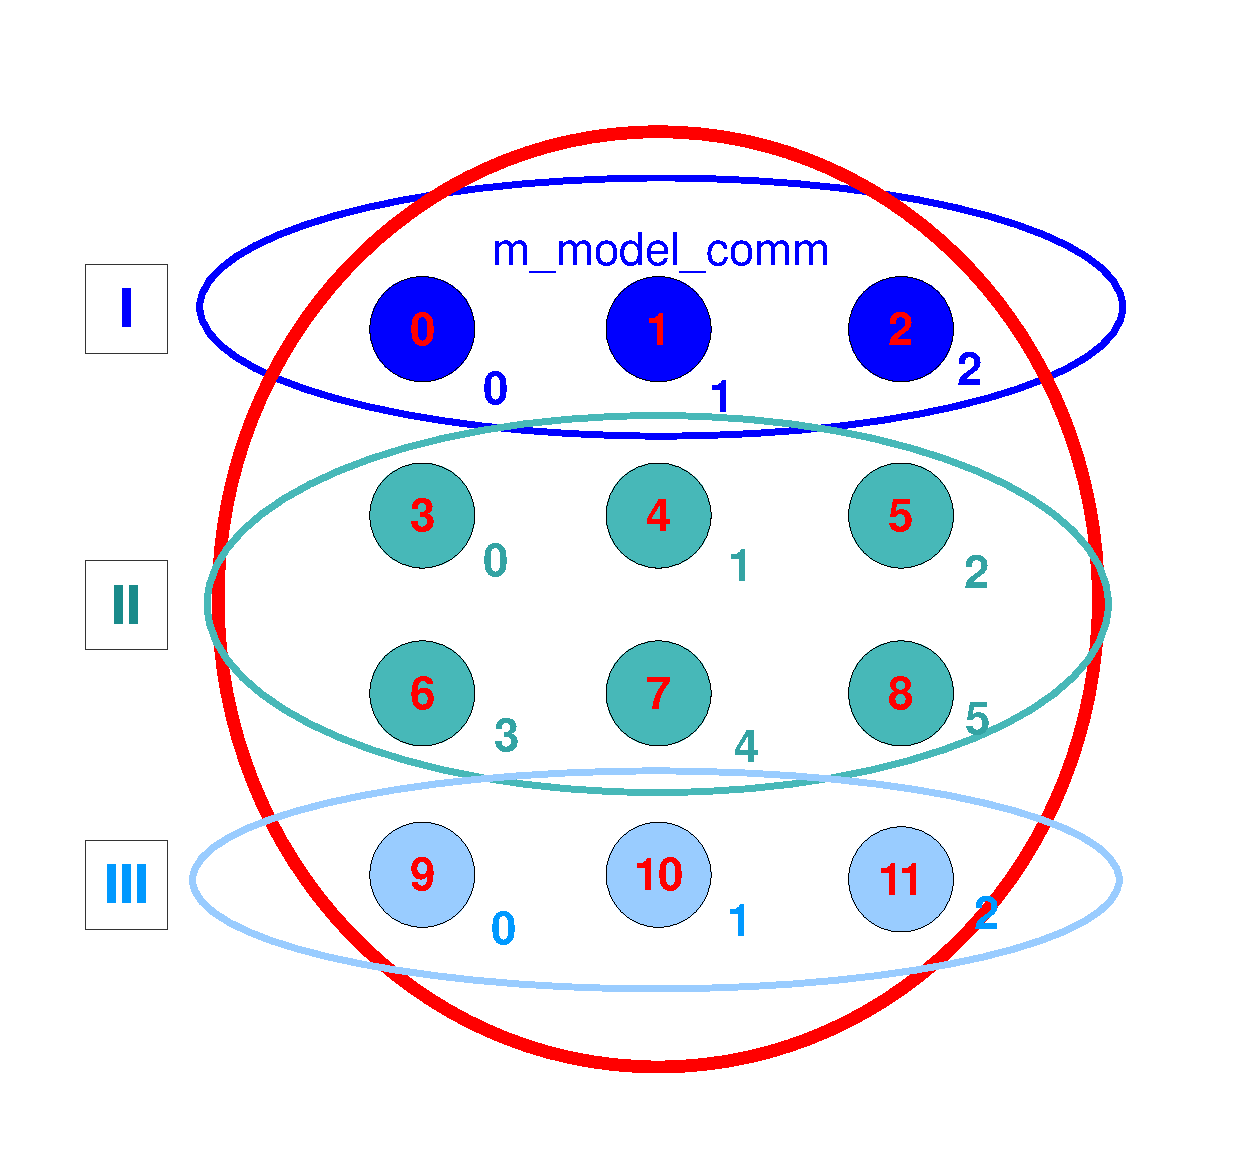
\includegraphics[width=0.8\textwidth]{MMDlib_MPIcomm.pdf} 
\end{center} 
\vspace*{-0.8cm}
\caption{Illustration of the variables defined in 
{\tt mmd\_handle\_communicator}:
The small circles symbolise the individual tasks. The red circle encloses all 
tasks visualising the global MPI-communicator ({\tt MPI\_comm\_world}).
The overall number of tasks {\tt m\_world\_npes} is 12 in this example. The rank
of each individual task in the global communicator ({\tt m\_world\_rank}) is 
indicated by the red numbers in the small circles. In this example the number of
coupled models ({\tt m\_NrOfCpl}) is 3. Each of the larger bluish ellipses 
indicates one model group communicator ({\tt m\_model\_comm}). For easier 
reference the models are indicated by roman numbers at the left hand side of 
the ellipses. The tasks are coloured identically to the ellipses. 
{\tt m\_model\_npes} is 3 for the models I and III, whereas it is 6 for model 
number II.
The number at the lower right of the small circles denotes the rank of the tasks
in the model group communicators ({\tt m\_model\_rank}). 
The {\tt start\_PE}s for the three models are the tasks with the MPI world rank 
0, 3 and 9, respectively. {\tt m\_my\_CPL\_Id} is 1 for the tasks 0-2 (rank
in the world communicator, red numbers) as they belong to model I. For model II
{\tt m\_my\_CPL\_Id} is 2 and for modell III it is 3.} 

\label{fig:MPIcomm} 
\end{figure*} 


\item After setting up the basic communicators the contents of the namelist,
 i.e., the \verb|name|, the \verb|Id| and the \verb|ParentId|,
are broadcasted to all PEs. The meaning of these variables is explained in the
example below.
\item Based on this information, the individual communicators for the direct 
communication between parent and child model(\verb|m_to_child_comm|) and 
vice versa (\verb|m_to_parent_comm|) are determined. As a Parent can feed
a number of child models, \verb|m_to_child_comm| is a 1-dimensional array
with dimension \verb|MMD_MAX_MODEL|. 
\item For chils models, the parent model type (\verb|m_ParentType|) is set
depending on the parent model name. \verb|m_ParentType| is an
 {\footnotesize INTEGER} and is set 
 to \verb|MMD_ParentIsECHAM|, if the parent name is 'echam' and to 
\verb|MMD_ParentIsCOSMO|, if it is 'cosmo'.
For future applications of the MMD library other {\footnotesize PARAMETERs}
 defining a parent model type can be added.

\item A parent model additionally needs a list of the Ids of its child
 models. This information
is stored in the 1-dimensional array \verb|MMD_Parent_for_Child|, which is
allocated by the number of child models a respective parent has to deal with.
\end{itemize}

\end{itemize}

\item {\tt MMD\_Print\_Error\_Message}:\\

\begin{tabular*}{0.94\textwidth}{@{\extracolsep\fill}|lllp{6cm}|}
\hline
\multicolumn{2}{|l}
{\tt SUBROUTINE  MMD\_Print\_Error\_Message} &
\multicolumn{2}{p{84mm}|}
{\tt (iu, MMD\_status)}\\
\hline
name & type & intent & description\\
\hline
%-----
\multicolumn{4}{|l|}{\bf mandatory arguments:}\\
iu & {\footnotesize INTEGER} & IN & unit for output \\
MMD\_status & {\footnotesize INTEGER} & IN & status flag \\
%-----
\hline
\end{tabular*}
\smallskip

      This is a utility subroutine printing individual error messages for
      predefined error stati. 

\item {\tt MMD\_FreeMem\_Communicator}:\\

\begin{tabular*}{0.94\textwidth}{@{\extracolsep\fill}|lllp{6cm}|}
\hline
\multicolumn{2}{|l}
{\tt SUBROUTINE MMD\_FreeMem\_Communicator} &
\multicolumn{2}{p{84mm}|}
{\tt ()}\\
\hline
\end{tabular*}
\smallskip

      At the very end of the model integration allocated memory needs to be
      released. This subroutine deallocates the memory allocated for 
      \verb|MMD_Parent_for_Child|.
\item {\tt PRIVATE read\_coupling\_layout}:\\

\begin{tabular*}{0.94\textwidth}{@{\extracolsep\fill}|lllp{6cm}|}
\hline
\multicolumn{2}{|l}
{\tt SUBROUTINE read\_coupling\_layout} &
\multicolumn{2}{p{84mm}|}
{\tt (MMD\_status)}\\
\hline
name & type & intent & description\\
\hline
%-----
\multicolumn{4}{|l|}{\bf mandatory arguments:}\\
MMD\_status & {\footnotesize INTEGER} & INOUT & error/status flag \\
%-----
\hline
\end{tabular*}
\smallskip
\vspace{1cm}

%****************
The subroutine \verb|read_coupling_layout| is called from the MMD subroutine
\verb|MMD_cag_model_communicator| as the coupling layout must be known for the 
communicator setup. The layout is determined by the user within the
MMD library namelist file \verb|MMD_layout.nml|. The required information is:
\begin{itemize}
\item the number of tasks associated to each individual model,
\item the type of the model (currently 'echam' for ECHAM5/MESSy or 'cosmo' for
COSMO/MESSy), and 
\item the parent ID of each model.
\end{itemize} 
An example is illustrated in Fig.\ 
\ref{fig:modeltree} with the global chemistry climate model ECHAM5/MESSy as 
{\it patriarch} und the regional COSMO/MESSy model as child models.
%\clearpage
%****************
\begin{figure*}
\begin{center} 
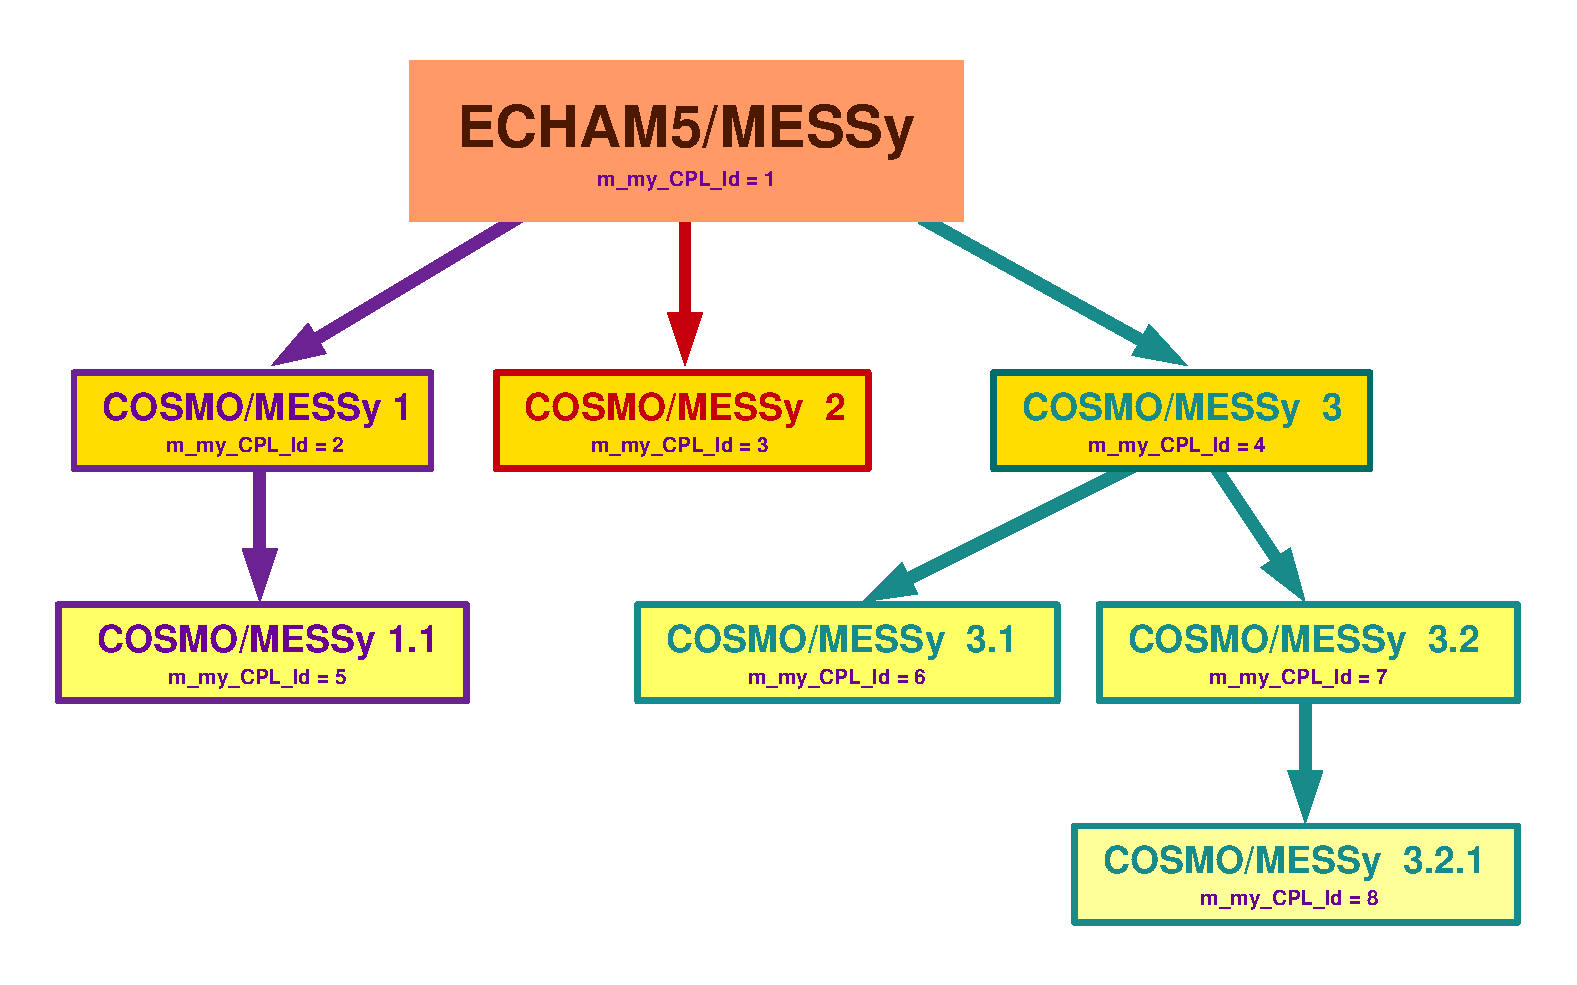
\includegraphics[width=\textwidth]{MMDlib_model_layout.pdf} 
\end{center} 
\vspace*{-2.95cm}
\begin{verbatim} 
       &CPL
       m_couplers(1)='echam', -1, $NPE[1]
       m_couplers(2)='cosmo',  1, $NPE[2]
       m_couplers(3)='cosmo',  1, $NPE[3]
       m_couplers(4)='cosmo',  1, $NPE[4]
       m_couplers(5)='cosmo',  2, $NPE[6]
       m_couplers(6)='cosmo',  4, $NPE[7]
       m_couplers(7)='cosmo',  4, $NPE[8]
       m_couplers(8)='cosmo',  7, $NPE[9]
       /
\end{verbatim} 
\vspace*{-0.5cm}
\caption{Example for a possible MMD model layout.} 
\label{fig:modeltree} 
\end{figure*} 
%****************

Each line defines one model within the MMD setup. \verb|m_couplers| is the 
variable name of the structure containing the setup information
within MMD. The index is the  model instance, i.e., the  MMD internal number or 
its \verb|Id|. It must be unique for each model.
The first column gives the name of the basemodel. The second column contains 
 the ID of the parent of the respective model (the so-called 
\verb|ParentId|). \verb|-1| in the entry for 'echam' signifies 
that this model has no parent model, in other words it is the {\it patriarch}.
The third column determines the number of Process Entities (PEs) required for 
each model\footnote{In the usual  ECHAM5/MESSy setup this is equivalent to 
{\tt NCPUS= NPROCA $\times$ NPROCB}, whereas for the COSMO model this is the 
product of {\tt nprocx} 
and {\tt nprocy}.}, these are usually set by the run-script.
In the example in Fig.\ \ref{fig:modeltree}, ECHAM5/MESSy 
(i.e., \verb|'echam'| in the namelist) is defined  as {\it patriarch}. It 
is Parent for the three COSMO/MESSy models with the MMD internal Ids 2,3,4.
 The MMD internal model number 5 is Child of the model with Id 2, 
i.e., ``COSMO/MESSy 1'' in our example
(Fig.\ \ref{fig:modeltree}). The MMD internal  
models number 6 and 7 are Children of the model number 4 (``COSMO/MESSy 3'' in 
Fig.\ \ref{fig:modeltree}).
Last but not least, the model with the internal number 8 is Child of the model
with Id 7 (``COSMO/MESSy 3.2'').

At the end of the subroutine \verb|read_coupling_layout|, after
reading the namelist file, the number of coupled models 
(\verb|m_NrOfCpl|) is determined according to the namelist settings.     
\end{itemize}



\subsubsection{{\tt mmd\_mpi\_wrapper}}\label{sec:mpiwrapper}

The module \verb|mmd_mpi_wrapper| provides six high level interface
routines for data exchange between child and parent models and
vice versa. Send and Receive for child and parent model are
managed by four subroutines:
\begin{itemize}
\item {\tt  MMD\_Send\_to\_Parent}:\\

\begin{tabular*}{0.95\textwidth}{@{\extracolsep\fill}|lllp{6.5cm}|}
\hline
\multicolumn{2}{|l}
{\tt SUBROUTINE MMD\_Send\_to\_Parent} &
\multicolumn{2}{p{84mm}|}
{\tt (buf, n, Parent\_rank, tag, ierr)}\\
\hline
name & type & intent & description\\
\hline
%-----
\multicolumn{4}{|l|}{\bf mandatory arguments:}\\
buf  &  {\footnotesize INTEGER, DIMENSION(:)}  & INOUT  & 1D integer data array to send\\
 &  {\footnotesize INTEGER, DIMENSION(:,:) }  &  INOUT & 2D integer data array to send \\
 & {\footnotesize  REAL(dp),  DIMENSION(:) }  &  INOUT & 1D real data array to send\\
&  {\footnotesize REAL(dp),  DIMENSION(:,:) }  &  INOUT & 2D real data array to send\\
& {\footnotesize  REAL(dp),  DIMENSION(:,:,:)}   &  INOUT & 3D real data array to send\\
n & {\footnotesize INTEGER}   & IN & length of buffer \\
Parent\_rank & {\footnotesize INTEGER} & IN  & rank of receiving Parent PE in the Parent group MPI-communicator\\
tag & {\footnotesize INTEGER}    & IN & tag for data transfer to unambiguously identify this data package \\
ierr & {\footnotesize INTEGER} & OUT & error flag \\
%%-----
\hline
\end{tabular*}
\smallskip

  This subroutine is called by a child model and sends a data array from
  the child to the parent model.

\item {\tt MMD\_Recv\_from\_Child}:\\

\begin{tabular*}{0.95\textwidth}{@{\extracolsep\fill}|lllp{6.5cm}|}
\hline
\multicolumn{2}{|l}
{\tt SUBROUTINE MMD\_Recv\_from\_Child} &
\multicolumn{2}{p{84mm}|}
{\tt (Child\_Id, buf, n, Child\_rank , tag, ierr)}\\
\hline
name & type & intent & description\\
\hline
%-----
\multicolumn{4}{|l|}{\bf mandatory arguments:}\\
Child\_Id & {\footnotesize INTEGER}   &  IN    &  ID of sending Child model \\
buf  &  {\footnotesize INTEGER, DIMENSION(:)}  & INOUT  & 1D integer data array to receive\\
 &  {\footnotesize INTEGER, DIMENSION(:,:) }  &  INOUT & 2D integer data array to receive \\
 &  {\footnotesize REAL(dp),  DIMENSION(:) }  &  INOUT & 1D real data array to receive\\
&  {\footnotesize REAL(dp),  DIMENSION(:,:) }  &  INOUT & 2D real data array to receive\\
& {\footnotesize  REAL(dp),  DIMENSION(:,:,:)}   &  INOUT & 3D real data array to receive\\
n & {\footnotesize INTEGER}   & IN & length of buffer \\
Child\_rank & {\footnotesize INTEGER} & IN  & rank of sending Child PE in the 
Child group MPI-communicator\\
tag & {\footnotesize INTEGER}    & IN & tag for data transfer to unambiguously identify this data package \\
ierr & {\footnotesize INTEGER} & OUT & error flag \\
%-----
%\multicolumn{4}{|l|}{\bf optional arguments:}\\
\hline
\end{tabular*}
\smallskip

  This subroutine is called by the parent model and 
receives a data array from the child model. 
\clearpage
\item {\tt  MMD\_Recv\_from\_Parent}:\\

\begin{tabular*}{0.95\textwidth}{@{\extracolsep\fill}|lllp{6.5cm}|}
\hline
\multicolumn{2}{|l}
{\tt SUBROUTINE MMD\_Recv\_from\_Parent} &
\multicolumn{2}{p{84mm}|}
{\tt (buf, n, Parent\_rank, tag, ierr)}\\
\hline
name & type & intent & description\\
\hline
%-----
\multicolumn{4}{|l|}{\bf mandatory arguments:}\\
buf  &  {\footnotesize INTEGER, DIMENSION(:)}  & INOUT  & 1D integer data array to receive\\
 &  {\footnotesize INTEGER, DIMENSION(:,:)  } &  INOUT & 2D integer data array to receive \\
 &  {\footnotesize REAL(dp),  DIMENSION(:)   }&  INOUT & 1D real data array to receive\\
&   {\footnotesize REAL(dp),  DIMENSION(:,:)  } &  INOUT & 2D real data array to receive\\
&  {\footnotesize  REAL(dp),  DIMENSION(:,:,:) }  &  INOUT & 3D real data array to receive\\
n & {\footnotesize INTEGER}   & IN & length of buffer \\
Parent\_rank & {\footnotesize INTEGER} & IN  & rank of sending Parent PE in the 
MPI group communicator for the Parent\\
tag & {\footnotesize INTEGER}    & IN & tag for data transfer to unambiguously identify this data package \\
ierr & {\footnotesize INTEGER} & OUT & error flag \\
%-----
\hline
\end{tabular*}
\smallskip

  This subroutine is called by the child model and 
receives a data array from the parent model.
\item {\tt MMD\_Send\_to\_Child}:\\

\begin{tabular*}{0.95\textwidth}{@{\extracolsep\fill}|lllp{6.5cm}|}
\hline
\multicolumn{2}{|l}
{\tt SUBROUTINE MMD\_Send\_to\_Child} &
\multicolumn{2}{p{84mm}|}
{\tt (Child\_Id, buf, n, Child\_rank , tag, ierr)}\\
\hline
name & type & intent & description\\
\hline
%-----
\multicolumn{4}{|l|}{\bf mandatory arguments:}\\
Child\_Id & {\footnotesize INTEGER}   &  IN    &  ID of Child model ({\it Receiver} of the data)\\
buf  &  {\footnotesize INTEGER, DIMENSION(:)}  & INOUT  & 1D integer data array to send\\
 &  {\footnotesize INTEGER, DIMENSION(:,:)}   &  INOUT & 2D integer data array to send\\
 &  {\footnotesize REAL(dp),  DIMENSION(:) }  &  INOUT & 1D real data array to send\\
&  {\footnotesize REAL(dp),  DIMENSION(:,:) }  &  INOUT & 2D real data array to send\\
&  {\footnotesize REAL(dp),  DIMENSION(:,:,:)}   &  INOUT & 3D real data array to send\\
n & {\footnotesize INTEGER}   & IN & length of buffer \\
Child\_rank & {\footnotesize INTEGER} & IN  & rank of receiving Child PE in 
the MPI group communicater for the Child model (Mostly rank = 0 is chosen.)\\
tag & {\footnotesize INTEGER}    & IN & tag for data transfer to unambiguously identify this data package \\
ierr & {\footnotesize INTEGER} & OUT & error flag\\
\hline
\end{tabular*}
\smallskip

  This subroutine is called by the parent and sends a data array from the 
  parent to the child model.
\end{itemize}
With these routines the user does not have to take care about the internal
MPI setup and the communicators. 
Moreover, the routines are overloaded for different data types:
 1D-\verb|integer| arrays, 
2D-\verb|integer| arrays and 1D-, 2D- and 3D-\verb|real| arrays, respectively.

In addition, two broadcasting subroutines have been implemented:
%\clearpage

\begin{itemize}
\item \verb|MMD_Inter_Bcast|:\\

\begin{tabular*}{0.95\textwidth}{@{\extracolsep\fill}|lllp{7.3cm}|}
\hline
\multicolumn{2}{|l}
{\tt SUBROUTINE MMD\_Inter\_Bcast} &
\multicolumn{2}{p{90mm}|}
{\tt (buf, sender [, Child\_Id] [, ierr])}\\
\hline
name & type & intent & description\\
\hline
%-----
\multicolumn{4}{|l|}{\bf mandatory arguments:}\\
buf  & {\footnotesize INTEGER}, DIMENSION(:) & INOUT & {\footnotesize
INTEGER} buffer to exchange \\
buf  & {\footnotesize CHARACTER(LEN=*)}  & INOUT &  {\footnotesize CHARACTER} buffer to exchange \\
%-----
\multicolumn{4}{|l|}{\bf optional arguments:}\\
Child\_Id & {\footnotesize INTEGER}   &  IN    & ID of ({\it remote}) Child (used by Parent only). \\
ierr       & {\footnotesize INTEGER}   &  OUT   & error flag\\
\hline
\end{tabular*}
\smallskip

This subroutine is called \verb|MMD_Inter_Bcast| and it provides the 
possibility to exchange 1-dimensional {\footnotesize INTEGER} or
{\footnotesize CHARACTER(LEN=*)} arrays between {\it remote models}.
The broadcasting subroutines can be easily overloaded to handle additional data 
types, so far there was no need to do so.

\item \verb|MMD_Bcast|:\\

\begin{tabular*}{0.95\textwidth}{@{\extracolsep\fill}|lllp{7.3cm}|}
\hline
\multicolumn{2}{|l}
{\tt SUBROUTINE MMD\_Bcast} &
\multicolumn{2}{p{90mm}|}
{\tt (buf, root\_pe [, comm] [, ierr])}\\
\hline
name & type & intent & description\\
\hline
%-----
\multicolumn{4}{|l|}{\bf mandatory arguments:}\\
buf & {\footnotesize INTEGER}         & INOUT  & {\footnotesize INTEGER} buffer to be broadcasted \\
    & {\footnotesize CHARACTER(LEN=*)} & INOUT &  {\footnotesize CHARACTER} buffer to  be broadcasted \\
root\_pe & {\footnotesize INTEGER}  & IN    & rank of the PE sending the data in the respective MPI group communicator \\
%-----
\multicolumn{4}{|l|}{\bf optional arguments:}\\
comm & {\footnotesize INTEGER} & IN   &  communicator \\
ierr & {\footnotesize INTEGER} & OUT  &  error flag \\
\hline
\end{tabular*}
\smallskip

The subroutine \verb|MMD_Bcast| can be used to broadcast 
{\footnotesize CHARACTER}
strings or {\footnotesize INTEGER} values using an arbitrary communicator. 
Thus, it can be used to broadcast data to PEs of the same model (using the
intra-model MPI-communicator, which is the default),
 to PEs of the {\it remote model} (set \verb|comm| in the parameter list to the 
communicator of the {\it remote model} (i.e., \verb|m_to_child_comm| or
\verb|m_to_parent_comm|, respectively), to both models of a Child-Parent Pair
(use the inter-communicator) or all models 
(set \verb|comm| to the world communicator).\\

\end{itemize}

%************************************************************************
%************************************************************************
\subsubsection{{\tt mmd\_child.f90}}\label{sec:mmd-child}
The Multi-Model-Driver (MMD) consists of two parts. The MMD library, which
is discussed here, and one MESSy submodel MMD2WAY consisting of the
sub-submodels MMD2WAY\_CHILD  and MMD2WAY\_PARENT dealing with child and
parent model side, respectively. The routines included in the MMD library module
\verb|mmd_child| contain the child model specific part of the MMD library and  
interact directly with the MESSy sub-submodel MMD2WAY\_CHILD.
\verb|mmd_child| includes thirteen subroutines and three functions:

\begin{itemize}
\item \verb|MMD_C_GetParentType|:\\
\vspace*{-0.3cm}

\begin{tabular*}{0.95\textwidth}{@{\extracolsep\fill}|lllp{9cm}|}
\hline
\multicolumn{2}{|l}
{\tt {\footnotesize INTEGER FUNCTION} MMD\_C\_GetParentType} &
\multicolumn{2}{p{84mm}|}
{\tt ()}\\
\hline
\end{tabular*}
\smallskip
\vspace*{-0.3cm}

The {\footnotesize INTEGER} function \verb|MMD_C_GetParentType| provides 
information about the associated parent model to the child MMD-subsubmodel.
It returns an {\footnotesize INTEGER} value indicating the type of the parent
model. 
At the time being this is one of \verb|MMD_ParentIsECHAM| or 
\verb|MMD_ParentIsCOSMO|. 

\item \verb|MMD_C_Init|:\\
\vspace*{-0.3cm}

\begin{tabular*}{0.95\textwidth}{@{\extracolsep\fill}|lllp{9cm}|}
\hline
\multicolumn{2}{|l}
{\tt SUBROUTINE MMD\_C\_Init} &
\multicolumn{2}{p{90mm}|}
{\tt (l2way)}\\
\hline
%\end{tabular*}
%\begin{tabular*}{0.95\textwidth}{@{\extracolsep\fill}|lllp{9cm}|}
name & type & intent & description\\
\hline
%-----
\multicolumn{4}{|l|}{\bf optional arguments:}\\
l2way & {\footnotesize LOGICAL} & IN & indicates if two-way coupling
is requested \\
%-----
\hline
\end{tabular*}
\smallskip
%\vspace*{-0.3cm}

At the beginning of the initialisation phase the child model side of the MMD
 library needs to be initialised, which is done in the
 subroutine \verb|MMD_C_Init|. The variable \verb|Me| of {\footnotesize TYPE} 
\verb|ExchDataDef| is declared in the \verb|mmd_child| module and
 provides all information required for the data exchange.

By calling the respective C-subroutine \verb|MMDc_C_Init| the number
of PEs occupied by the {\it remote model} is evaluated. 
The structure component \verb|Me%PEs| and the  MMD internal
variable \verb|BufLen|, which stores the length of  
the buffer received from each parent PE, are allocated according to
the number of {\it remote PEs}. 
All {\footnotesize POINTER}s, which are not yet ASSOCIATEd are NULLIF(Y)ied, 
i.e., \verb|Me%Ar|, \verb|Me%ArrayStart| and \verb|Me%PEs(:)%locInd|
are NULLIF(Y)ied.  
All structure components \verb|Me%PEs(:)%NrEle| and the variable
\verb|BufLen(:)| are initialised with zero.

If 2-way coupling is employed, the same initialisation steps are
performed with the variable  \verb|Parent| containing the information for the
(back-)coupling to the Parent.

Additionally, the information whether this child model couples back to its
parent model is stored in a module wide variable \verb|ltwoway|. This
information is provided by the optional argument \verb|l2way|. If it
is not present, 1-way coupling is assumed (\verb|ltwoway=.FALSE.|).  
%\clearpage
\item  \verb|MMD_C_Set_DataArray_Name|:\\
\vspace*{-0.3cm}

\begin{tabular*}{0.95\textwidth}{@{\extracolsep\fill}|lllp{7cm}|}
\hline
\multicolumn{2}{|l}
{\tt SUBROUTINE MMD\_C\_Set\_DataArray\_Name} &
\multicolumn{2}{p{89mm}|}
{\tt (par\_channel, par\_object, chld\_channel, chld\_object, chld\_repr, istat)}\\
\hline
\end{tabular*}
\begin{tabular*}{0.95\textwidth}{@{\extracolsep\fill}|lllp{7cm}|}
name & type & intent & description\\
\hline
%-----
\multicolumn{4}{|l|}{\bf mandatory arguments:}\\
par\_channel & {\footnotesize CHARACTER(LEN=*)} & IN & name of Parent {\it channel} \\
par\_object  & {\footnotesize CHARACTER(LEN=*)} & IN & name of Parent {\it channel object} \\
chld\_channel & {\footnotesize CHARACTER(LEN=*)} & IN & name of Child {\it channel} \\
chld\_object  & {\footnotesize CHARACTER(LEN=*)} & IN & name of Child {\it channel object} \\
chld\_repr    & {\footnotesize CHARACTER(LEN=*)} & IN & {\it representation} of Child {\it channel object} as given in the namelist \\
istat    & {\footnotesize INTEGER} & OUT & error/status flag \\
%-----
\hline
\end{tabular*}
\smallskip
%\vspace*{-0.3cm}

The list of {\it exchange fields},
which is determined by the sub-submodel MMD2WAY\_CHILD, needs to be initialised 
within the MMD library. MMD2WAY\_CHILD reads a namelist containing a
list of {\it exchange fields}, i.e., a list of those files required by
the child model from the parent model.
The subroutine \verb|MMD_C_Set_DataArray_Name| builds a concatenated list of
these fields.
 The structure component \verb|Me%ArrayStart| points to the memory of the first 
 {\it exchange field}, whereas all data arrays are
 stored in the concatenated list \verb|Me%Ar|. The {\it channel} and {\it channel
 object} names of the {\it exchange fields} are stored in the structure 
components \verb|Me%Ar%Arrdef%channel| and \verb|Me%Ar%Arrdef%object|, 
respectively.
Additionally, the parent {\it channel} and {\it channel object} names, the 
child {\it representation} as given in the MMD2WAY\_CHILD namelist
file, and an index are broadcasted to the parent model.

\item  \verb|MMD_C_Set_DataArray_EndList|:\\
\vspace*{-0.3cm}

\begin{tabular*}{0.95\textwidth}{@{\extracolsep\fill}|lllp{6.0cm}|}
\hline
\multicolumn{2}{|l}
{\tt SUBROUTINE MMD\_C\_Set\_DataArray\_EndList} &
\multicolumn{2}{p{75mm}|}
{\tt ()}\\
\hline
\end{tabular*}
\smallskip
\vspace*{-0.3cm}

When all data fields are initialised, the end of the list is indicated by 
calling the subroutine \verb|MMD_C_Set_DataArray_EndList|.
In this subroutine the coupling index is set to \verb|-1|. This value is 
interpreted as list end on the parent model side of the library.

\item \verb|MMD_C_Get_ParDataArray_Name|:\\
\vspace*{-0.3cm}

\begin{tabular*}{0.95\textwidth}{@{\extracolsep\fill}|lllp{7.5cm}|}
\hline
\multicolumn{2}{|l}
{\tt  SUBROUTINE MMD\_C\_Get\_ParDataArray\_Name} &
\multicolumn{2}{p{75mm}|}
{\tt (numfields)}\\
\hline
\end{tabular*}
\begin{tabular*}{0.95\textwidth}{@{\extracolsep\fill}|lllp{7.5cm}|}
name & type & intent & description\\
\hline
%-----
\multicolumn{4}{|l|}{\bf mandatory arguments:}\\
 numfields & {\footnotesize INTEGER} & OUT &  number of fields
 requested by the Parent \\
%-----
\hline
\end{tabular*}
\smallskip

For the coupling of the data fields from the child to the parent model, the
 {\it channel} and {\it channel object} names of the {\it exchange
 fields} on the child model side, the {\it representation} name as provided
 by the parent model (given as namelist parameter), the required
 interpolation method, and a logical flag, indicating if the unit of the
 requested field is required by the parent, must be received by the
 child from its parent model. Within the subroutine 
\verb|MMD_C_Get_ParDataArray_Name| these information are acquired from
 the parent model by \verb|MMD_Bcast|s.
First the \verb|couple_index| is received. A value of \verb|-1| indicates the
end of the transmission of the list and the subroutine is exited.
Based on the received data the concatenated list (part of
the \verb|ExchDataDef| structure) defining the individual data fields
is established. 
The memory location of the first array is stored in the variable 
\verb|Parent%ArrayStart|. The child {\it channel} and {\it channel object}
 names and the parent {\it representation} name are stored in the structure 
components \verb|Parent%Ar%ArrDef%channel|,  
\verb|Parent%Ar%ArrDef%object| 
and \verb|Parent%Ar%ArrDef%repr|, respectively, making these strings
available for later use on the parent part of the MMD library.
Additionally, the structure components \verb|Parent%Ar%ArrDef%interpM|
and \verb|Parent%Ar%ArrDef%l_sentunit| store the requested interpolation
method and the request for the fields unit, respectively.

%\clearpage
\item \verb|MMD_C_GetNextParArray|:\\
\vspace*{-0.3cm}

\begin{tabular*}{0.95\textwidth}{@{\extracolsep\fill}|lllp{6.5cm}|}
\hline
\multicolumn{2}{|l}
{\tt LOGICAL FUNCTION MMD\_C\_GetNextParArray} &
\multicolumn{2}{p{84mm}|}
{\tt (MyChannel, myName, repr, interpM, l\_SentUnit)}\\
\hline
\end{tabular*}
\begin{tabular*}{0.95\textwidth}{@{\extracolsep\fill}|lllp{6.5cm}|}
name & type & intent & description\\
\hline
%-----
\multicolumn{4}{|l|}{\bf mandatory arguments:}\\
 MyChannel & CHARACTER(LEN=*) & OUT & name of {\it channel}  \\
myName     &  CHARACTER(LEN=*) & OUT & name of {\it channel object} \\
repr       & CHARACTER(LEN=*)  & OUT  & parent representation of the field \\
interpM    &  INTEGER  & OUT & interpolation method \\
l\_SentUnit & LOGICAL  & OUT & sent unit of field to parent \\
%-----
\hline
\end{tabular*}
\smallskip

After the call of the subroutine \verb|MMD_C_Get_ParDataArray_Name|
the information about the field requested by the parent model are
available in a concatenated list. The
function \verb|MMD_C_GetNextParArray| makes this information
available. With each call of this function the child model steps along the
concatenated list and provides the information of the current list
element. These are the {\it channel} and {\it channel object} name of
the field in the child model, the representation of the field in the
parent model, the requested interpolation method, and the logical indicating
if the parent requires the unit of the field in the child model.

As long as new elements are available in the concatenated
list,  \verb|MMD_C_GetNextParArray| is \verb|.TRUE.|.
If the end of the list is reached,  \verb|MMD_C_GetNextParArray| is
set to \verb|.FALSE.|.

\item \verb|MMD_C_Set_ParIndexlist|:\\
\vspace*{-0.3cm}

\begin{tabular*}{0.95\textwidth}{@{\extracolsep\fill}|lllp{6cm}|}
\hline
\multicolumn{2}{|l}
{\tt SUBROUTINE MMD\_C\_Set\_ParIndexlist} &
\multicolumn{2}{p{90mm}|}
{\tt (index\_list, fractions, wfunc)}\\
\hline
\end{tabular*}
\begin{tabular*}{0.95\textwidth}{@{\extracolsep\fill}|lllp{6cm}|}
name & type & intent & description\\
\hline
%-----
\multicolumn{4}{|l|}{\bf mandatory arguments:}\\
index\_list & {\footnotesize INTEGER, DIMENSION(:,:)} &INOUT & index
list (used for the horizontal element association) as calculated from
the Child submodel \\ 
fractions  & {\footnotesize REAL, DIMENSION(:,:)} &IN           & \\
wfunc      & {\footnotesize REAL, DIMENSION(:,:)} &IN, OPTIONAL & \\
%-----
\hline
\end{tabular*}
\smallskip

The most tricky part of the MMD library is the association of grid points from 
the parallel decomposed child ``out''-field\footnote{As the interpolation from
the child model to the parent grid is performed by the 
child model, the data fields sent by the child model are already on the
parent grid. This field will be called ``out''-field in the
following. In case of MECO(n) the grid of the ``out''-field is the
same as the grid of the ``in''-field.} (the field to sent) with
the grid points on the parallel decomposed Parent fields (the received
field). 

For that, the child submodel MMD2WAY\_CHILD sends the geographical
longitude and  
the geographical latitude fields of the parallel decomposed parent
 {\it out-grid}\footnote{As the {\it in-} and {\it out-grid} can be rotated
 grids, the geographical longitude and latitude fields are 2D fields each.},
 each as three  
dimensional fields: The first two ranks spread the horizontal
distribution of the 
 geographical longitude or latitude fields, respectively, as defined on one 
PE, the third rank is the respective PE number in the model specific 
MPI-group-communicator, i.e., the blue numbers at the lower right side of the
PEs in Fig.\ \ref{fig:MPIcomm}. These fields
 contain for each index triple (i$_c$,j$_c$, PE$_c$) the geographical
 coordinates. 
 Based on the geographical coordinates, the parent submodel MMD2WAY\_PARENT
 identifies for each of the child ``out''-grid points the respective grid point
 in the local parent model domain, thus adding to the list the parent process 
number PE$_p$ (of the model specific MPI-communicator) on which the respective 
geographical point is located and the 
respective index pair  (i$_p$,j$_p$) in the local domain.
Thus a list of $n$ sextuples (i$_p$,j$_p$,i$_c$,j$_c$,PE$_c$, PE$_p$)$_n$  
containing the index pairs of both decomposed fields and the child and the
 parent PE number is created, with $n$ being the overall number of exchanged 
horizontal elements.

This list is sent to MMD2WAY\_CHILD which forwards it as parameter to
 the  MMD library subroutine \verb|MMD_C_Set_ParIndexlist|, where it
 is further analysed to yield all the information
required for a most efficient data exchange. Additionally, a 2D-field
 (\verb|fraction|) in ``out''-grid geometry is parameter to the
 subroutine, indicating 
 which fraction of each grid box of the ``out''-grid is actually
 covered by the local child domain. The third parameter of the
 subroutine is the weight function (\verb|wfunc|) containing the
 weight which should be applied when changing the original parent
 field. This weighting function is 1 (100\%) in most of the domain and
 diminishing to 0 at the border of the child model domain.

At the beginning, the task of 
\verb|m_model_rank=0| sorts the index list by the child model PE numbers and 
calculates the number of grid points each child PE has to sent 
(\verb|Parent%NrPoints|). This number is sent to the respective child PE. 
Additionally, the part of the index list of the respective child PE
 is sent to it.
Each child PE deduces from its part of the index list the number of 
horizontal elements \verb|Parent%PEs(ip)%NrEle| it has to send to 
each individual parent PE. After that, the index pairs of the local child grid 
 associated with the horizontal elements are saved 
in the \verb|locInd| structure \verb|Parent%PEs(ip)%locInd|. Additionally,
the index pairs of the local parent grid, the fraction and the weight
function of the respective element are saved in the respective components of
the local structure variable \verb|par_ind|.  
In the following the number of horizontal elements and the components
of the local variable \verb|par_ind| are exchanged with the respective
parent PEs.

Note: As the buffer exchange is based on the index list as explained above,
the buffer exchange can only be used for fields which contain both horizontal
dimensions. If other fields should be exchanged during a simulation, this has to
be performed via the subroutines provided by the module \verb|mmd_mpi_wrapper|
(Sect.\ \ref{sec:mpiwrapper}).


\item \verb|MMD_C_Set_ParDataArray|:\\
\vspace*{-0.3cm}

\begin{tabular*}{0.95\textwidth}{@{\extracolsep\fill}|lllp{6cm}|}
\hline
\multicolumn{2}{|l}
{\tt SUBROUTINE MMD\_C\_Set\_ParDataArray} &
\multicolumn{2}{p{83mm}|}
{\tt (status, DimLen, ArrayOrder, p4)}\\
\hline
\end{tabular*}
\begin{tabular*}{0.95\textwidth}{@{\extracolsep\fill}|lllp{6cm}|}
name & type & intent & description\\
\hline
%-----
\multicolumn{4}{|l|}{\bf mandatory arguments:}\\
status & {\footnotesize INTEGER} & OUT & status flag \\
DimLen & {\footnotesize INTEGER,DIMENSION(4)} & IN & length of the 4 dimensions \\
ArrayOrder & {\footnotesize CHARACTER(LEN=4)} & IN & {\it axis string} indicating order of axes \\
p4 & {\footnotesize REAL(DP), DIMENSION(:,:,:,:)}& {\footnotesize POINTER} & {\footnotesize POINTER} for 4D data arrays \\
%-----
\hline
\end{tabular*}
\smallskip
\vspace*{-0.3cm}

 The subroutine \verb|MMD_C_Set_ParDataArray| is called for each of the
 fields individually. It associates the respective {\footnotesize
 POINTER} of the array and stores 
\begin{itemize}
\item  the dimension lengths (\verb|Parent%Ar%ArrDef%dim|),
\item  the order of dimensions (\verb|Parent%Ar%ArrDef%dim_order|), and
\item  calculates the axis indices \verb|Parent%Ar%ArrDef%xyzn_dim|.
\end{itemize}
 Additionally,
\begin{itemize} 
\item the array length (\verb|Parent%Ar%Arrdef%ArrLen(ip)|),
\item  the array index (\verb|Parent%Ar%Arrdef%ArrIdx(ip)|), and 
\item the buffer length (\verb|ParBufLen(ip)|)
\end{itemize}
are calculated from the above information.
Subsect.\ \ref{sec:example} illustrates the meaning of these variables.

\item \verb|MMD_C_Get_Indexlist|:\\
\vspace*{-0.3cm}

\begin{tabular*}{0.95\textwidth}{@{\extracolsep\fill}|lllp{6cm}|}
\hline
\multicolumn{2}{|l}
{\tt SUBROUTINE MMD\_C\_Get\_Indexlist} &
\multicolumn{2}{p{75mm}|}
{\tt ()}\\
\hline
\end{tabular*}
\smallskip
\vspace*{-0.3cm}

The most important contribution of the parent model to the data
exchange, apart from 
the data itself, is the list attributing the data points of the parallel 
decomposed parent grid to the parallel decomposed child {\it in-grid}. 
The parent calculates the index list, which
interlinks the data grid point ($i_p$,$j_p$) on parent process PE$_p$ with the 
child process PE$_c$ and the local {\it in-field} grid box ($i_c$,$j_c$)
(see description to Fig.\ \ref{fig:MMD-NrEle}, Table \ref{tab:ex1} and Sect.\
 \ref{sec:mmd-parent}).
The subroutine \verb|MMD_C_Get_Indexlist| processes the data made available
by the parent model. Each parent PE sends the number of elements \verb|NrEle|,
which will be sent during the buffer exchange to the respective child PE.
Accordingly, this information is stored in the structure component 
\verb|Me%PEs(ip)%NrEle|.
 Subsequently, the index pairs associated to the elements
are sent from the parent and stored in \verb|Me%PEs(ip)%locInd|. Here,
\verb|ip| is the number of the respective sending parent PE.

\item  \verb|MMD_C_Get_Repr|:\\
\vspace*{-0.3cm}

\begin{tabular*}{0.95\textwidth}{@{\extracolsep\fill}|lllp{6.cm}|}
\hline
\multicolumn{2}{|l}
{\tt SUBROUTINE  MMD\_C\_Get\_Repr} &
\multicolumn{2}{p{76mm}|}
{\tt (axis, gdimlen, name, att)}\\
\hline
\end{tabular*}
\begin{tabular*}{0.95\textwidth}{@{\extracolsep\fill}|lllp{6.cm}|}
name & type & intent & description\\
\hline
%-----
\multicolumn{4}{|l|}{\bf mandatory arguments:}\\
axis &  {\footnotesize CHARACTER(LEN=4)} & OUT & string indicating axes order \\
gdimlen &  {\footnotesize INTEGER, DIMENSION(4)} & OUT & length of dimensions \\
name & {\footnotesize CHARACTER(LEN=STRLEN\_CHANNEL)} & OUT & {\it representation} name \\
att &  {\footnotesize CHARACTER(LEN=STRLEN\_ULONG)}   & OUT & {\it channel 
object} {\it attribute} (e.g.\ height axis) \\ 
%-----
\hline
\end{tabular*}
\smallskip
%\vspace*{-0.3cm}

After the internal setup of the MMD library, the memory for the {\it in-fields}
needs to be initialised within the child MESSy submodel MMD2WAY\_CHILD and the 
{\footnotesize POINTER} to this memory is handed to the MMD library.
The allocation of the memory within MMD2WAY\_CHILD is described in detail within the
``MMD user manual''\footnote{The MMD user manual is available in the same 
electronic supplement as this manual.}. In order to enable the
 exchange of fields, which {\it representation} is not a priori known, the 
subroutine \verb|MMD_C_Get_Repr| (in \verb|mmd_child)| and 
\verb|MMD_P_Sent_Repr| (in \verb|mmd_parent)| have been added to the MMD library
 to exchange the information required to determine
the {\it representation} on the child model side from the information
given by the parent model. These routines are only called, if the {\it
representation} in the  
MMD2WAY\_CHILD namelist file was set to \verb|'#UNKNOWN'|.
In this case the parent sends the {\it representation} name of the respective 
Parent {\it channel object}. Additionally,
\begin{itemize}
\item  the {\it axis string},
\item  the  global {\it dimensions}, and 
\item an additional {\it attribute} (e.g., emission heights)
\end{itemize}
are exchanged. 
These parameters are made available on the Child side within the subroutine 
\verb|MMD_C_Get_Repr| and handed to the MMD2WAY\_CHILD submodel via parameter list.

\item  \verb|MMD_C_GetNextArray|:\\
\vspace*{-0.3cm}

\begin{tabular*}{0.95\textwidth}{@{\extracolsep\fill}|lllp{6.5cm}|}
\hline
\multicolumn{2}{|l}
{\tt LOGICAL FUNCTION MMD\_C\_GetNextArray} &
\multicolumn{2}{p{84mm}|}
{\tt (MyChannel, myName)}\\
\hline
\end{tabular*}
\begin{tabular*}{0.95\textwidth}{@{\extracolsep\fill}|lllp{6.5cm}|}
name & type & intent & description\\
\hline
%-----
\multicolumn{4}{|l|}{\bf mandatory arguments:}\\
 MyChannel & CHARACTER(LEN=*) & OUT & name of {\it channel}  \\
myName     &  CHARACTER(LEN=*) & OUT & name of {\it channel object} \\
%-----
\hline
\end{tabular*}
\smallskip
\vspace*{-0.3cm}

After the allocation of the memory required by the child model submodel, the 
respective {\footnotesize POINTER}s can be made available to the MMD library.
For this the child model steps along the concatenated list provided by
MMD with the 
help of the MMD function \verb|MMD_C_GetNextArray|. This function provides
the required {\it channel} and {\it channel object} name to the child submodel 
MMD2WAY\_CHILD. With each call, this function internally steps one entry 
forward within the concatenated list.
\clearpage
\item  \verb|MMD_C_Set_DataArray|:\\
\vspace*{-0.3cm}

\begin{tabular*}{0.95\textwidth}{@{\extracolsep\fill}|lllp{6cm}|}
\hline
\multicolumn{2}{|l}
{\tt SUBROUTINE MMD\_C\_Set\_DataArray} &
\multicolumn{2}{p{83mm}|}
{\tt (status, DIMLEN, ArrayOrder, p4)}\\
\hline
\end{tabular*}
\begin{tabular*}{0.95\textwidth}{@{\extracolsep\fill}|lllp{6cm}|}
name & type & intent & description\\
\hline
%-----
\multicolumn{4}{|l|}{\bf mandatory arguments:}\\
status & {\footnotesize INTEGER} & OUT & status flag \\
DimLen & {\footnotesize INTEGER,DIMENSION(4)} & IN & length of the 4 dimensions \\
ArrayOrder & {\footnotesize CHARACTER(LEN=4)} & IN & {\it axis string} indicating order of axes \\
p4 & {\footnotesize REAL(DP), DIMENSION(:,:,:,:)}& {\footnotesize POINTER} & {\footnotesize POINTER} for 4D data arrays \\
%-----
\hline
\end{tabular*}
\smallskip
\vspace*{-0.3cm}

 The subroutine \verb|MMD_C_Set_DataArray| is called for each of the
 fields individually. It associates the respective {\footnotesize POINTER} of the array and stores
\begin{itemize}
\item  the dimension lengths (\verb|Me%Ar%ArrDef%dim|),
\item  the order of dimensions (\verb|Me%Ar%ArrDef%dim_order|), and
\item  calculates the axis indices \verb|Me%Ar%ArrDef%xyzn_dim|.
\end{itemize}
 Additionally,
\begin{itemize} 
\item the array length (\verb|Me%Ar%Arrdef%ArrLen(ip)|),
\item  the array index (\verb|Me%Ar%Arrdef%ArrIdx(ip)|), and 
\item the buffer length (\verb|BufLen(ip)|)
\end{itemize}
are calculated from the above information.
Subsect.\ \ref{sec:example} illustrates the meaning of these variables.

\item  \verb|MMD_C_SetInd_and_AllocMem|:\\
\vspace*{-0.3cm}

\begin{tabular*}{0.95\textwidth}{@{\extracolsep\fill}|lllp{6cm}|}
\hline
\multicolumn{2}{|l}
{\tt SUBROUTINE MMD\_C\_SetInd\_and\_AllocMem} &
\multicolumn{2}{p{84mm}|}
{\tt ()}\\
\hline
\end{tabular*}
\smallskip
\vspace*{-0.3cm}

When the definition of all data fields within the Fortran95 interface of the
MMD library is complete, the
subroutine \verb|MMD_C_SetInd_and_AllocMem| must be called to
initialise the total length of the buffers within the C-core of the
library. The total buffer 
length corresponds to the memory that must be allocated for the buffer exchange
 (see Sect.\ \ref{sec:CCHILD}).
As the amount of the required memory is defined differently in the
cases of 1-way or 2-way coupling, different C functions are called
depending on the coupling type. 

At this point, all preparations are complete and the data exchange can be 
performed.
 
\item  \verb| MMD_C_GetBuffer|:\\
\vspace*{-0.3cm}

\begin{tabular*}{0.95\textwidth}{@{\extracolsep\fill}|lllp{6cm}|}
\hline
\multicolumn{2}{|l}
{\tt SUBROUTINE MMD\_C\_GetBuffer } &
\multicolumn{2}{p{93mm}|}
{\tt (WaitTime)}\\
\hline
\end{tabular*}
\begin{tabular*}{0.95\textwidth}{@{\extracolsep\fill}|lllp{6.5cm}|}
name & type & intent & description\\
\hline
%-----
\multicolumn{4}{|l|}{\bf optional arguments:}\\
WaitTime & REAL(dp) & OUT & time waiting until buffer is available \\
\hline
\end{tabular*}
\smallskip

To actually exchange the data from parent to the child model during
the integration phase, the parent writes the required data into the
memory buffers made available by \verb|MPI_alloc_mem|.
To read these buffers, the subroutine \verb|MMD_C_GetBuffer| calls,
independently for each parent PE, its C counterpart  
\verb|MMDc_C_GetBuffer| (see Fig.\ \ref{fig:MMD-workflow}). 
The C function hands back a 1-dimensional array. This is transferred back into 
its full 4-dimensional structure within the Fortran95 part of the library.
 For this back transformation the indices for the different {\it dimensions} and 
the \verb|dim_order| label are used (see Sect.\ \ref{sec:example}).
\verb|MMD_C_GetBuffer| contains a generic routine for the back transition
of the 1-dimensional arrays to all dimension orders. In addition, more 
computationally efficient implementations for the most often used {\it
representations} are provided as special cases, e.g.\ the standard axis orders
  \verb|'XY--'| and \verb|'XYZ-'|.
By transforming the fields sent by each parent PE into their usual 4D structure,
 the {\it in-fields} of the child submodel are filled and can be processed 
by the child submodel afterwards.
During the integration, this subroutine can be called as often as required.


\item \verb|SUBROUTINE MMD_C_FillBuffer|
%\vspace*{-0.3cm}

\begin{tabular*}{0.95\textwidth}{@{\extracolsep\fill}|lllp{9cm}|}
\hline
\multicolumn{2}{|l}
{\tt  SUBROUTINE MMD\_C\_FillBuffer} &
\multicolumn{2}{p{90mm}|}
{\tt ( )}\\
\hline
\end{tabular*}
\smallskip

If two-way coupling is ongoing,
the subroutine \verb|MMD_C_FillBuffer| fills the buffer within the
time loop.
The C function actually filling the buffer requires a 1-dimensional array as
 input.  Thus the 4-dimensional data needs to be re-ordered. As the dimension 
order of the child arrays is not a priori known on the parent side, the
packing algorithm in \verb|MMD_C_FillBuffer| packs the arrays
 invariably in the same order:
\begin{itemize}
\item The loop over the elements in the 
xy-plane (\verb|NrEle|) is the slowest,
\item  next is the loop over the \verb|'Z'| 
dimension, and
\item fastest varying is the \verb|'N'| dimension. 
\end{itemize}
The \verb|MMD_C_FillBuffer| contains an algorithm packing an array of arbitrary 
order of {\it dimensions} in grid point {\it representation}\footnote{It is 
presumed that the array is defined in the 
horizontal space as the buffer exchange only works in this case.}.
For higher computing efficiency, the commonly used {\it dimension orders} are 
implemented as special cases (e.g.\ \verb|'XY--'|, \verb|'XZY-'|
or \verb|'XYZN'|). If required, other special cases can be included in this
subroutine as well. For each 1-dimensional (i.e.\ packed) array per {\it remote 
PE} 
the C routine \verb|MMDc_C_FillBuffer| is called, copying the array to the
memory space allocated by \verb|MPI_Alloc_mem|. 
When all buffers attributed to all parent PEs are filled, the C function
\verb|MMDc_C_SetBarrier| is called, which sets a barrier to prevent the buffer 
to be filled a second time before the data was read by the parent.


\item  \verb|MMD_C_FreeMem|:\\
\vspace*{-0.3cm}

\begin{tabular*}{0.95\textwidth}{@{\extracolsep\fill}|lllp{6cm}|}
\hline
\multicolumn{2}{|l}
{\tt SUBROUTINE MMD\_C\_FreeMem} &
\multicolumn{2}{p{84mm}|}
{\tt ()}\\
\hline
\end{tabular*}
\smallskip
\vspace*{-0.3cm}

After the integration, the memory allocated during the initialisation phase 
 is deallocated. This is done within the subroutine \verb|MMD_C_FreeMem|.
\end{itemize}

\subsubsection{{\tt mmd\_parent.f90}}\label{sec:mmd-parent}

The module \verb|mmd_parent| contains the parent model specific Fortran95
part of the MMD library. In contrast to
the child model side, the parent can provide data to more than one child model.
Therefore, many of the structures used in the child submodel require an array 
dimension for the parent side.
In the following, two indices to identify a specific child model are
distinguished: 
\begin{itemize}
\item The variable \verb|ChildId| always indicates the index of the child
 model in the entire MMD setup. This is dimensioned by the 
{\footnotesize PARAMETER} \verb|MMD_MAX_MODEL|, which is set to 64 at
the moment.  
The association of the \verb|ChildId| depends on the entries in the MMD 
namelist file \verb|MMD_layout.nml|. In \verb|mmd_parent| this index is used to 
address the correct child model communicator (\verb|m_to_child_comm|), and
the index is parameter of almost all calls of the subroutines of the C
part of the MMD library, because the C part of the library uses
exclusively this index (see Sect. \ref{sec:MMD-C}). 
\item After the initial setup of MMD the number of child models for each
 individual parent is known. Thus, the data definition structure (and other 
variables the parent has to define for each child model separately) are 
dimensioned by the number of child models of the respective
parent. \verb|Id| is the index used to address the child specific data
structure of the specific parent.
\end{itemize}

Hereafter, the subroutines provided by the module \verb|mmd_parent|
are listed. All routines, except \verb|MMD_P_Allocate_Child| and 
\verb|MMD_P_FreeMem| are called separately for each child model. 
Thus one of the two indices introduced above (\verb|ChildId| or \verb|Id|) is
always parameter of the subroutine calls to identify the respective
 child model.


\begin{itemize}
\item \verb|MMD_P_Allocate_Child|:\\
\vspace*{-0.3cm}

\begin{tabular*}{0.95\textwidth}{@{\extracolsep\fill}|lllp{9cm}|}
\hline
\multicolumn{2}{|l}
{\tt SUBROUTINE MMD\_P\_Allocate\_Child} &
\multicolumn{2}{p{90mm}|}
{\tt (NumChildren, l2way)}\\
\hline
\end{tabular*}
\begin{tabular*}{0.95\textwidth}{@{\extracolsep\fill}|lllp{9cm}|}
name & type & intent & description\\
\hline
%-----
\multicolumn{4}{|l|}{\bf mandatory arguments:}\\
NumChildren & {\footnotesize INTEGER} & IN & number of Child models \\
l2way & {\footnotesize LOGICAL} & IN & .TRUE. if backward coupling of Child
models is required \\
%-----
\hline
\end{tabular*}
\smallskip

At the very beginning, in the subroutine \verb|MMD_P_Allocate_Child| a 
pointer of {\footnotesize TYPE} 
\verb|ExchDataDef| (named \verb|Child|) is allocated according to the
number of child models served by the specific parent
model. Additionally, the variable 
for the length of the exchange buffer (\verb|ChldBL|) to the respective
child model needs to be dimensioned also by the number of child models.
If \verb|l2way == .TRUE.|, coupling back of at least some child model is
required, and the structure \verb|Parent| of {\footnotesize
TYPE} \verb|ExchDataDef| needs to be allocated to the number of
child models (not only those which are coupled back).
 The buffer length variable \verb|ParBL| is allocated accordingly. 
Furthermore, the structure components, which are pointers, are
NULLIF(Y)ied.

Last but not least, the information, if the simulation is a 1-way or a
2-way coupled simulation is saved in a module wide variable
(\verb|ltwoway =l2way|). 

\item  \verb|MMD_P_Init|:\\
 This subroutine is called separately for each child of a parent.

\begin{tabular*}{0.95\textwidth}{@{\extracolsep\fill}|lllp{9cm}|}
\hline
\multicolumn{2}{|l}
{\tt SUBROUTINE MMD\_P\_Init} &
\multicolumn{2}{p{90mm}|}
{\tt (ChildId, Id)}\\
\hline
\end{tabular*}
\begin{tabular*}{0.95\textwidth}{@{\extracolsep\fill}|lllp{9cm}|}
name & type & intent & description\\
\hline
%-----
\multicolumn{4}{|l|}{\bf mandatory arguments:}\\
ChildId & {\footnotesize INTEGER} & IN & index of child model within the overall MMD model setup\\
Id & {\footnotesize INTEGER} & IN & index of child model in the child list of this specific parent\\
%-----
\hline
\end{tabular*}
\smallskip

First, the parent needs to be initialised for each child model. The subroutine
\verb|MMD_P_Init| inquires the number of processes occupied by the respective 
child model (\verb|Child(Id)%inter_npes|) by calling the MMD
subroutine \verb|MMDc_P_Init| and 
allocates \verb|Child(Id)%PEs|  and \verb|ChldBL(Id)%BufLen|,
accordingly.
\verb|Child(Id)%PEs(ip)%NrEle| and \verb|ChldBL(Id)%BufLen(ip)| are
 initialised with 0 (\verb|ip| is the index
of the {\it remote PE}) and \verb|Child(Id)%PEs(ip)%locInd|  is
 NULLIF(Y)ied. 

In case of 2-way coupling, the information acquired
for \verb|Child(Id)| are also saved in the respective \verb|Parent(Id)|
structure components, i.e. \verb|Parent(Id)%ChildId|
and \verb|Parent(Id)%inter_npes| are set. The structure components
of \verb|Parent(Id)| are preset in the same way as those of \verb|Child(Id)|.

\item  \verb|MMD_P_Set_Indexlist|:\\
\vspace*{-0.3cm}

\begin{tabular*}{0.95\textwidth}{@{\extracolsep\fill}|lllp{7cm}|}
\hline
\multicolumn{2}{|l}
{\tt SUBROUTINE MMD\_P\_Set\_Indexlist} &
\multicolumn{2}{p{90mm}|}
{\tt (Id, index\_list)}\\
\hline
\end{tabular*}
\begin{tabular*}{0.95\textwidth}{@{\extracolsep\fill}|lllp{7cm}|}
name & type & intent & description\\
\hline
%-----
\multicolumn{4}{|l|}{\bf mandatory arguments:}\\
Id & {\footnotesize INTEGER} & IN &  index of child model in the child
model list of this specific parent \\
index\_list & {\footnotesize INTEGER, DIMENSION(:,:)} &INOUT & index list (used for the horizontal element association) as calculated by the parent submodel \\ 
%-----
\hline
\end{tabular*}
\smallskip

The most tricky part of the MMD library is the association of grid points of 
the parallel decomposed parent grid with
the grid points of the parallel decomposed child model {\it in-grid}. 
For that, the parent submodel MMD2WAY\_PARENT receives the
geographical longitude and  
the geographical latitude fields of the parallel decomposed child  
 ``in''-grid\footnote{As the parent and the child model ``in''-grids
 can be rotated 
 grids, the geographical longitude and latitude fields are 2D fields each.},
 each as three dimensional fields: The first two ranks spread the
 horizontal distribution of the 
 geographical longitude or latitude fields, respectively, as defined on one 
PE, the third rank is the respective PE number in the model specific 
MPI-group-communicator, i.e., the blue numbers at the lower right side of the
PEs in Fig.\ \ref{fig:MPIcomm}. These fields
 contain for each index triple (i$_c$,j$_c$, PE$_c$) the geographical
 coordinates. 
 Based on the geographical coordinates, the parent 
submodel identifies for each of the child grid points the respective grid point
 in the local parent model domain, thus adding to the list the parent process 
number PE$_p$ (of the model specific MPI-communicator) on which the respective 
geographical point is located and the 
respective index pair  (i$_p$,j$_p$) in the local domain.
Thus a list of $n$ sextuples (i$_p$,j$_p$,i$_c$,j$_c$,PE$_c$, PE$_p$)$_n$  
containing the index pairs in both decomposed fields, and the child and the
 parent PE number is created, with $n$ being the overall number of exchanged 
horizontal elements.

This list is further analysed within the MMD library routine
 \verb|MMD_P_Set_Indexlist| to yield all the information
required for a most efficient data exchange. At the beginning, the task of 
\verb|m_model_rank=0| sorts the index list by the parent PE numbers and 
calculates the number of grid points  each parent PE has to sent 
(\verb|Child(Id)%NrPoints|). This number is sent to the respective parent PE. 
Additionally, the part of the index list of the respective parent PE
 is sent to it.
Each parent PE deduces from its part of the index list the number of 
horizontal elements \verb|Child(Id)%PEs(ip)%NrEle| it has to send to 
each individual child PE. After that, the index pairs of the local parent grid 
 associated with the horizontal elements are saved 
in the \verb|locInd| structure \verb|Child(Id)%PEs(ip)%locInd|, and the index 
pairs of the local Child grid are saved in an intermediate variable. 
Next, the number of horizontal elements and the
intermediate variables are exchanged with the respective child PEs. 

Note: As the buffer exchange is based on the index list as explained above,
the buffer exchange can only be used for fields, which contain both horizontal
dimensions. If other fields should be exchanged during a simulation, this has to
be performed via the subroutines provided by the module \verb|mmd_mpi_wrapper|
(Sect.\ \ref{sec:mpiwrapper}).
%\clearpage
\item \verb|MMD_P_Get_ParIndexlist|:\\
\vspace*{-0.3cm}

\begin{tabular*}{0.95\textwidth}{@{\extracolsep\fill}|lllp{7cm}|}
\hline
\multicolumn{2}{|l}
{\tt  SUBROUTINE MMD\_P\_Get\_ParIndexlist} &
\multicolumn{2}{p{90mm}|}
{\tt (Id, fractions, wfunc)}\\
\hline
\end{tabular*}
\begin{tabular*}{0.95\textwidth}{@{\extracolsep\fill}|lllp{7cm}|}
name & type & intent & description\\
\hline
%-----
\multicolumn{4}{|l|}{\bf mandatory arguments:}\\
Id & {\footnotesize INTEGER} & IN &  index of child model in the child
list of this specific parent \\
fractions &  {\footnotesize REAL(dp)} & {\footnotesize POINTER} &
grid box wise fractional overlap by the respective child model PE \\
wfunc &  {\footnotesize REAL(dp)} & {\footnotesize POINTER} & weight
function \\
%-----
\hline
\end{tabular*}
\smallskip

This subroutine establishes the \verb|Indexlist| for the coupling of the
child model data to the parent. First, from each individual child model PE
the number of elements provided by this PE is received by the parent.
This number is stored in the structure component 
\verb|Parent(Id)%PEs(ip)%NrEle|. Subsequently, 
\verb|Parent(Id)%PEs(ip)%locInd| and two local variables are allocated
accordingly. The latter are used to receive the information about the local
index pair (\verb|(i,j)|), the fractions and the weight
functions. The index pair is stored in the structure component 
\verb|Parent(Id)%PEs(ip)%locInd|, while the fraction and the weight
function are copied to the subroutine parameter \verb|fraction|
and \verb|wfunc|. 
\clearpage
\item \verb|MMD_P_Set_ParDataArray_Name|:\\
\vspace*{-0.3cm}

\begin{tabular*}{0.95\textwidth}{@{\extracolsep\fill}|lllp{7cm}|}
\hline
\multicolumn{2}{|l}
{\tt SUBROUTINE MMD\_P\_Set\_ParDataArray\_Name} &
\multicolumn{2}{p{70mm}|}
{\tt (par\_channel, par\_object, chld\_channel, chld\_object,
chld\_repr, interpol\_method, sentunit, istat)}\\
\hline
\end{tabular*}
\begin{tabular*}{0.95\textwidth}{@{\extracolsep\fill}|lllp{7cm}|}
name & type & intent & description\\
\hline
%-----
\multicolumn{4}{|l|}{\bf mandatory arguments:}\\
Id     & {\footnotesize INTEGER} & IN & child model Id \\
par\_channel & {\footnotesize CHARACTER(LEN=*)} & IN & name of parent {\it channel} \\
par\_object  & {\footnotesize CHARACTER(LEN=*)} & IN & name of parent {\it channel object} \\
chld\_channel & {\footnotesize CHARACTER(LEN=*)} & IN & name of child {\it channel} \\
chld\_object  & {\footnotesize CHARACTER(LEN=*)} & IN & name of child {\it channel object} \\
chld\_repr    & {\footnotesize CHARACTER(LEN=*)} & IN & {\it
representation} of child {\it channel object} as given in the
namelist \\
interpol\_method &  {\footnotesize INTEGER} & IN & indicator for
interpolation method used for interpolation between child and parent
{\it representation} for this field\\
sentunit &  {\footnotesize LOGICAL} & IN & Is the unit of the child field
required by parent? \\
istat    & {\footnotesize INTEGER} & OUT & error/status flag \\
%-----
\hline
\end{tabular*}
\smallskip
%\vspace*{-0.3cm}

The list of {\it exchange fields} requested by the parent,
which is determined by the sub-submodel MMD2WAY\_PARENT, needs to be
initialised within the MMD library. MMD2WAY\_PARENT reads a namelist
containing a list of {\it exchange fields}, i.e., a list of those
files required by the parent model from the respective child model.
The subroutine \verb|MMD_P_Set_ParDataArray_Name| is called seperately
for each of these fields and builds a concatenated list of pointers to
these fields.
The structure component \verb|Parent(Id)%ArrayStart| points to the
memory of the first {\it exchange field}, whereas all data arrays are
stored in the concatenated list \verb|Parent(Id)%Ar|. The {\it
channel} and {\it channel object} names of the {\it exchange fields}
are stored in the structure components 
\verb|Parent(Id)%Ar%Arrdef%channel|
and \verb|Parent(Id)%Ar%Arrdef%object|, respectively.
Additionally, the {\it channel} and {\it channel object} name of these
fields in the child model, their {\it representation}s -as given in the
MMD2WAY\_PARENT namelist file-, the interpolation methods, and the
indicators, signifying if the field units need to be sent to the parent, are
broadcasted to the child model. 

\item  \verb|MMD_P_Set_ParDataArray_EndList|:\\
\vspace*{-0.3cm}

\begin{tabular*}{0.95\textwidth}{@{\extracolsep\fill}|lllp{6.0cm}|}
\hline
\multicolumn{2}{|l}
{\tt SUBROUTINE MMD\_P\_Set\_ParDataArray\_EndList} &
\multicolumn{2}{p{75mm}|}
{\tt (Id)}\\
\hline
\end{tabular*}
\begin{tabular*}{0.95\textwidth}{@{\extracolsep\fill}|lllp{7.5cm}|}
name & type & intent & description\\
\hline
%-----
\multicolumn{4}{|l|}{\bf mandatory arguments:}\\
Id & {\footnotesize INTEGER} & IN &  index of child model in the child
list of this specific parent model \\
%-----
\hline
\end{tabular*}
\smallskip

When all data fields are initialised, the end of the list is indicated by 
calling the subroutine \verb|MMD_P_Set_ParDataArray_EndList|.
In this subroutine the coupling index is set to \verb|-1|. This value is 
interpreted as list end from the child model side of the library.

 %\clearpage
\item  \verb|MMD_P_Get_DataArray_Name|:\\
\vspace*{-0.3cm}

\begin{tabular*}{0.95\textwidth}{@{\extracolsep\fill}|lllp{7cm}|}
\hline
\multicolumn{2}{|l}
{\tt  SUBROUTINE MMD\_P\_Get\_DataArray\_Name} &
\multicolumn{2}{p{90mm}|}
{\tt (Id)}\\
\hline
\end{tabular*}
\begin{tabular*}{0.95\textwidth}{@{\extracolsep\fill}|lllp{7cm}|}
name & type & intent & description\\
\hline
%-----
\multicolumn{4}{|l|}{\bf mandatory arguments:}\\
Id & {\footnotesize INTEGER} & IN &  index of child model in the child list of this specific parent model\\
%-----
\hline
\end{tabular*}
\smallskip

For the coupling of the data fields required by the child model, the
 {\it channel} and {\it channel object} 
 names of the {\it exchange fields} and the {\it representation} name
 listed in the namelist of the child model must be received by 
 the parent from each child model. Within the subroutine 
\verb|MMD_P_Get_DataArray_Name| the {\it channel} and {\it channel object}
 names and the {\it representation} name are acquired from the child model by
 \verb|MMD_Bcast|s.
First the \verb|couple_index| is received. A value of \verb|-1| indicates the
end of the transmission of the list and the subroutine is exited.
Based on the received data, the concatenated list (part of the \verb|ExchDataDef|
 structure) defining the individual data fields is established.
The memory location of the first array is stored in the variable 
\verb|Child(Id)%ArrayStart|. The parent {\it channel} and {\it channel object}
 name and the child {\it representation} name are stored in the structure 
components \verb|Child(Id)%Ar%ArrDef%channel|,  
\verb|Child(Id)%Ar%ArrDef%object| 
and \verb|Child(Id)%Ar%ArrDef%repr|, respectively, making these strings
available for later use on the parent model side of the MMD library.

\item  \verb|MMD_P_GetNextArray|:\\
\vspace*{-0.3cm}

\begin{tabular*}{0.95\textwidth}{@{\extracolsep\fill}|lllp{7cm}|}
\hline
\multicolumn{2}{|l}
{\tt LOGICAL FUNCTION MMD\_P\_GetNextArray} &
\multicolumn{2}{p{90mm}|}
{\tt (Id, MyChannel, myName, repr)}\\
\hline
\end{tabular*}
\begin{tabular*}{0.95\textwidth}{@{\extracolsep\fill}|lllp{7cm}|}
name & type & intent & description\\
\hline
%-----
\multicolumn{4}{|l|}{\bf mandatory arguments:}\\
Id & {\footnotesize INTEGER} & IN &  index of child model in the child list of this specific parent model\\
MyChannel & {\footnotesize CHARACTER(LEN=*)} & OUT & parent {\it channel} name of data field\\
myName & {\footnotesize CHARACTER(LEN=*)} & OUT & parent {\it channel object} name of data field\\
repr & {\footnotesize CHARACTER(LEN=*)} & OUT & {\it representation}
of data field (as given by the child model)\\
%-----
\hline
\end{tabular*}
\smallskip

So far, the {\it channel} and {\it channel object} names as requested
 by the child model are only known within the MMD library itself. For
 the acquisition of the parent model fields, they must be made
 available for the parent submodel MMD2WAY\_PARENT. 
With each call to the function \verb|MMD_P_GetNextArray| the next element
of the concatenated list is addressed, and the {\it channel} and {\it channel 
object} name and the {\it representation} name as provided by the child model
 are forwarded to the parent submodel MMD2WAY\_PARENT. The parent
 submodel obtains the requested data {\footnotesize POINTER} based on
 the {\it channel} and {\it channel object} name by calling the
 subroutine \verb|get_channel_object| of the MESSy infrastructure
 submodel CHANNEL. 
%\clearpage
\item  \verb|MMD_P_Send_Repr|:\\
\vspace*{-0.3cm}

\begin{tabular*}{0.95\textwidth}{@{\extracolsep\fill}|lllp{5cm}|}
\hline
\multicolumn{2}{|l}
{\tt SUBROUTINE MMD\_P\_Send\_Repr} &
\multicolumn{2}{p{74mm}|}
{\tt (axis, gdimlen, name, att, ChildId)}\\
\hline
\end{tabular*}
\begin{tabular*}{0.95\textwidth}{@{\extracolsep\fill}|lllp{5.5cm}|}
name & type & intent & description\\
\hline
%-----
\multicolumn{4}{|l|}{\bf mandatory arguments:}\\
axis&{\footnotesize CHARACTER(LEN=4)}&INOUT& {\it axis string} of {\it representation}\\
gdimlen&{\footnotesize INTEGER}, DIMENSION(4)&INOUT& global {\it dimensions} of  {\it representation}\\
name&{\footnotesize CHARACTER(LEN=STRLEN\_CHANNEL)}&INOUT& name of  {\it representation}\\
att&{\footnotesize CHARACTER(LEN=STRLEN\_ULONG)}&INOUT& {\it attribute} of data object\\
ChildId &{\footnotesize INTEGER}&IN& index of the respective child
model in the MMD model setup\\
%-----
\hline
\end{tabular*}
\smallskip

If the {\it representation} name sent by the child model
is \verb|"#UNKOWN"|, the child requests further information about the
{\it representation} of the  
respective {\it channel object} from the parent model (see description of the 
subroutine \verb|MMD_C_Get_Repr| in Sect.\ \ref{sec:mmd-child}).
The MMD library routine \verb|MMD_P_Send_Repr| sends the 
\begin{itemize}
\item {\it axis string},
\item the global {\it dimensions},
\item the name of the {\it representation}, and 
\item an additional  {\it attribute}
\end{itemize}
 to the child model.
\clearpage
\item  \verb|MMD_P_Set_DataArray|:\\
\vspace*{-0.3cm}

\begin{tabular*}{0.95\textwidth}{@{\extracolsep\fill}|lllp{7cm}|}
\hline
\multicolumn{2}{|l}
{\tt SUBROUTINE MMD\_P\_Set\_DataArray} &
\multicolumn{2}{p{90mm}|}
{\tt (Id, status, DIMLEN, ArrayOrder, p4)}\\
\hline
\end{tabular*}
\begin{tabular*}{0.95\textwidth}{@{\extracolsep\fill}|lllp{7cm}|}
name & type & intent & description\\
\hline
%-----
\multicolumn{4}{|l|}{\bf mandatory arguments:}\\
Id & {\footnotesize INTEGER} & IN &  index of child model in the child list of this specific parent model\\
status &{\footnotesize INTEGER} & OUT & error/status flag \\
DimLen & {\footnotesize INTEGER, DIMENSION(4)} & IN & dimension length of input array \\
ArrayOrder & {\footnotesize CHARACTER(LEN=4)} & IN & {\it axis string} for input array \\
p4 & {\footnotesize  REAL(DP), DIMENSION(:,:,:,:)} & {\footnotesize POINTER} & 4D {\footnotesize {\footnotesize POINTER}} to the 
memory of the {\it exchange field}\\
%-----
\hline
\end{tabular*}
\smallskip

For the coupling of the data requested by the child model, the
 {\footnotesize POINTER} to the memory of the parent model 
 {\it exchange fields} are passed to the 
MMD library by the subroutine \verb|MMD_P_Set_DataArray| and saved in the
structure component \verb|Child(Id)%Ar%Arrdef%p4|.
Additionally,
\begin{itemize}
\item the dimensions (\verb|Child(Id)%Ar%Arrdef%dim|), 
\item the dimension order (\verb|Child(Id)%Ar%Arrdef%dim_order|) and 
\item the index of the \verb|'X'|, \verb|'Y'|, \verb|'Z'| and \verb|'N|' axes 
(\verb|Child(Id)%Ar%ArrDef%xyzn_dim|)
\end{itemize}
 are stored within the \verb|Child| structure. Making use of these information,
for each child model PE (index \verb|ip|) the individual array length 
(\verb|Child(Id)%Ar%Arrdef%ArrLen(ip)|) and the length of the buffer
sent by each parent model PE to each child PE are calculated
 (\verb|ChldBL(Id)%BufLen(ip)|).  


\item  \verb|MMD_P_GetNextParArray|:\\
\vspace*{-0.3cm}

\begin{tabular*}{0.95\textwidth}{@{\extracolsep\fill}|lllp{6.5cm}|}
\hline
\multicolumn{2}{|l}
{\tt LOGICAL FUNCTION MMD\_P\_GetNextParArray} &
\multicolumn{2}{p{84mm}|}
{\tt (Id, MyChannel, myName)}\\
\hline
\end{tabular*}
\begin{tabular*}{0.95\textwidth}{@{\extracolsep\fill}|lllp{6.5cm}|}
name & type & intent & description\\
\hline
%-----
\multicolumn{4}{|l|}{\bf mandatory arguments:}\\
Id & {\footnotesize INTEGER} & IN &  index of child model in the child list of this specific parent model\\
 MyChannel & CHARACTER(LEN=*) & OUT & name of {\it channel}  \\
myName     &  CHARACTER(LEN=*) & OUT & name of {\it channel object} \\
%-----
\hline
\end{tabular*}
\smallskip
%\vspace*{-0.3cm}

After the allocation of the memory required by the parent submodel for
the coupling of the data requested by the parent, the  
respective {\footnotesize POINTER}s can be made available to the MMD
library.
For this, the MMD function \verb|MMD_P_GetNextParArray| steps along
the concatenated list provided by MMD. Within the function, a library
internal pointer is set to the current list member. Additionally, this
function provides the required {\it channel} and {\it channel object}
name to the parent submodel  
MMD2WAY\_PARENT. With each call, this function internally steps one entry 
forward within the concatenated list.


\item  \verb|MMD_P_Set_ParDataArray|:\\
\vspace*{-0.3cm}

\begin{tabular*}{0.95\textwidth}{@{\extracolsep\fill}|lllp{6cm}|}
\hline
\multicolumn{2}{|l}
{\tt SUBROUTINE MMD\_P\_Set\_ParDataArray} &
\multicolumn{2}{p{83mm}|}
{\tt (Id, status, DIMLEN, ArrayOrder, p4)}\\
\hline
\end{tabular*}
\begin{tabular*}{0.95\textwidth}{@{\extracolsep\fill}|lllp{6cm}|}
name & type & intent & description\\
\hline
%-----
\multicolumn{4}{|l|}{\bf mandatory arguments:}\\
Id & {\footnotesize INTEGER} & IN &  index of child model in the child list of this specific parent model\\
status & {\footnotesize INTEGER} & OUT & status flag \\
DimLen & {\footnotesize INTEGER,DIMENSION(4)} & IN & length of the 4 dimensions \\
ArrayOrder & {\footnotesize CHARACTER(LEN=4)} & IN & {\it axis string} indicating order of axes \\
p4 & {\footnotesize REAL(DP), DIMENSION(:,:,:,:)}& {\footnotesize POINTER} & {\footnotesize POINTER} for 4D data arrays \\
%-----
\hline
\end{tabular*}
\smallskip
\vspace*{-0.3cm}

 The subroutine \verb|MMD_P_Set_ParDataArray| is called for each of the
 fields individually, making use of the MMD internal pointers set by
 the function \verb|MMD_P_GetNextParArray|. It associates the
 respective {\footnotesize POINTER} of the array and stores 
\begin{itemize}
\item  the dimension lengths (\verb|Parent%Ar%ArrDef%dim|),
\item  the order of dimensions (\verb|Parent%Ar%ArrDef%dim_order|), and
\item  the calculated the axis indices (in \verb|Parent%Ar%ArrDef%xyzn_dim|).
\end{itemize}
 Additionally,
\begin{itemize} 
\item the array length (\verb|Parent%Ar%Arrdef%ArrLen(ip)|),
\item  the array index (\verb|Parent%Ar%Arrdef%ArrIdx(ip)|), and 
\item the buffer length (\verb|ParBL(Id)%BufLen(ip)|)
\end{itemize}
are calculated from the above information. \verb|ip| is the index of
the respective child model PE.
Subsect.\ \ref{sec:example} illustrates the meaning of these variables.

\item  \verb|MMD_P_SetInd_and_AllocMem|:\\
\vspace*{-0.3cm}

\begin{tabular*}{0.95\textwidth}{@{\extracolsep\fill}|lllp{8.9cm}|}
\hline
\multicolumn{2}{|l}
{\tt  SUBROUTINE MMD\_P\_SetInd\_and\_AllocMem} &
\multicolumn{2}{p{89mm}|}
{\tt (Id)}\\
\hline
\end{tabular*}
\begin{tabular*}{0.95\textwidth}{@{\extracolsep\fill}|lllp{8.9cm}|}
name & type & intent & description\\
\hline
%-----
\multicolumn{4}{|l|}{\bf mandatory arguments:}\\
Id & {\footnotesize INTEGER} & IN &  index of child model in the child list of this specific parent model\\
%-----
\hline
\end{tabular*}
\smallskip

After all {\footnotesize POINTER}s and dimension information are
stored, the size of the buffer for the exchange with the {\it remote
model} is determined. For a 1-way coupling, this buffer length is
equal to the sum over all buffer lengths sent to the individual child
PEs (\verb|SUM(ChldBL(Id)%BufLen)|). If 2-way coupling is required,
data is exchanged in both directions. Thus, the exchange buffer needs
to be dimensioned as required by the larger of the two exchange data
sets \verb|MAX(SUM(ChldBL(Id)%BufLen),SUM(ParBL(Id)%BufLen))|.
 This is triggered by the call of the
 subroutine \verb|MMDc_P_SetInd_and_Mem|
 or \verb|MMDc_P_SetInd_and_Mem_2way|, respectively.
As the full size of the buffer is only required in the C part of the library 
the Fortran95 subroutine  \verb|MMD_P_SetInd_and_AllocMem| simply
calls the C function \verb|MMDc_P_SetInd_and_Mem|.
After processing this subroutine the initialisation phase is finished.

\item  \verb|MMD_P_FillBuffer|:\\
\vspace*{-0.3cm}

\begin{tabular*}{0.95\textwidth}{@{\extracolsep\fill}|lllp{9cm}|}
\hline
\multicolumn{2}{|l}
{\tt  SUBROUTINE MMD\_P\_FillBuffer} &
\multicolumn{2}{p{90mm}|}
{\tt (Id [, WaitTime])}\\
\hline
\end{tabular*}
\begin{tabular*}{0.95\textwidth}{@{\extracolsep\fill}|lllp{9cm}|}
name & type & intent & description\\
\hline
%-----
\multicolumn{4}{|l|}{\bf mandatory arguments:}\\
Id & {\footnotesize INTEGER} & IN &  index of child model in the child list of this specific parent model\\
%-----
\multicolumn{4}{|l|}{\bf optional arguments:}\\
WaitTime & {\footnotesize REAL(dp)} & OUT & idle time in seconds waiting for buffer release\\
\hline
\end{tabular*}
\smallskip

Within the time loop the subroutine \verb|MMD_P_FillBuffer| fills the buffer.
The C function actually filling the buffer requires a 1-dimensional array as
 input.  Thus the 4-dimensional data needs to be re-ordered. As the dimension 
order of the parent arrays is not a priori known on the child model side, the
packing algorithm in \verb|MMD_P_FillBuffer| packs the arrays
 invariably in the same order:
\begin{itemize}
\item The loop over the elements in the 
xy-plane (\verb|NrEle|) is the slowest,
\item  next is the loop over the \verb|'Z'| 
dimension, and
\item fastest varying is the \verb|'N'| dimension. 
\end{itemize}
The \verb|MMD_P_FillBuffer| contains an algorithm packing an array of arbitrary 
order of {\it dimensions} in grid point {\it representation}\footnote{It is 
presumed that the array is defined in the 
horizontal space as the buffer exchange only works in this case.}.
For higher computing efficiency, the commonly used {\it dimension orders} are 
implemented as special cases (e.g.\ \verb|'XY--'|, \verb|'XZY-'|
or \verb|'XYZN'|). If required, other special cases can be included in this
subroutine as well. For each 1-dimensional (i.e.\ packed) array per {\it remote 
PE} 
the C routine \verb|MMDc_P_FillBuffer| is called, copying the array to the
memory space allocated by \verb|MPI_Alloc_mem|. 
When all buffers attributed to all child model PEs are filled, the C function
\verb|MMDc_P_SetBarrier| is called, which sets a barrier to prevent the buffer 
to be filled a second time before the data was read by the child model.

During the integration, this subroutine can be called as often as
required, but only in turns with the
subroutines \verb|MMD_C_GetBuffer|, \verb|MMD_C_FillBuffer|
and \verb|MMD_P_FillBuffer| for the 2-way coupling, or in case of 1-way
coupling in turns with \verb|MMD_C_GetBuffer|. 
 
\item  \verb| MMD_P_GetBuffer|:\\
\vspace*{-0.3cm}

\begin{tabular*}{0.95\textwidth}{@{\extracolsep\fill}|lllp{6cm}|}
\hline
\multicolumn{2}{|l}
{\tt SUBROUTINE MMD\_P\_GetBuffer } &
\multicolumn{2}{p{93mm}|}
{\tt (Id, WaitTime)}\\
\hline
\end{tabular*}
\begin{tabular*}{0.95\textwidth}{@{\extracolsep\fill}|lllp{6.5cm}|}
name & type & intent & description\\
\hline
%-----
\multicolumn{4}{|l|}{\bf mandatory arguments:}\\
Id & {\footnotesize INTEGER} & IN &  index of child model in the child list of this specific parent model\\
\multicolumn{4}{|l|}{\bf optional arguments:}\\
WaitTime & REAL(dp) & OUT & time waiting until buffer is available \\
\hline
\end{tabular*}
\smallskip

To actually exchange the data from the child to the parent model during
the integration phase, the child model writes the required data to the
memory buffers made available by \verb|MPI_alloc_mem|.
To read this buffers the subroutine \verb|MMD_P_GetBuffer| calls
independently for each child PE its C counterpart  
\verb|MMDc_P_GetBuffer| (see Fig.\ \ref{fig:MMD-workflow}). 
The C function hands back a 1-dimensional array. This is transferred back into 
its 4-dimensional structure within the Fortran95 part of the library.
 For this back transformation the indices for the different {\it
 dimensions} and  
the \verb|dim_order| label are used (see Sect.\ \ref{sec:example}).
\verb|MMD_P_GetBuffer| contains a generic routine for the back transition
of the 1-dimensional arrays to all dimension orders. In addition, more 
computationally efficient implementations for the most often used {\it
representations} are provided as special cases, e.g.\ the standard axis orders
  \verb|'XY--'| and \verb|'XYZ-'|.
By transforming the fields sent by each child model PE into their
 4D structure,
 the {\it in-fields} of the parent submodel are filled and can be processed 
by the parent submodel afterwards.
During the integration, this subroutine can be called as often as
required, but only in turns with the
subroutines \verb|MMD_P_FillBuffer|, \verb|MMD_C_GetBuffer|
and \verb|MMD_C_FillBuffer|. 

\item  \verb|MMD_P_FreeMem|:\\
\vspace*{-0.3cm}

\begin{tabular*}{0.95\textwidth}{@{\extracolsep\fill}|lllp{7cm}|}
\hline
\multicolumn{2}{|l}
{\tt SUBROUTINE MMD\_P\_FreeMem} &
\multicolumn{2}{p{90mm}|}
{\tt (NumChildren)}\\
\hline
\end{tabular*}
\begin{tabular*}{0.95\textwidth}{@{\extracolsep\fill}|lllp{7cm}|}
name & type & intent & description\\
\hline
%-----
\multicolumn{4}{|l|}{\bf mandatory arguments:}\\
NumChildren & {\footnotesize INTEGER} & IN & number of child models of this specific parent model\\
%-----
\hline
\end{tabular*}
\smallskip

At the end of the simulation the allocated memory is deallocated within the 
subroutine \verb|MMD_P_FreeMem|.

\end{itemize}

\subsubsection{{\tt mmd\_test.f90}}

The most tricky parts of the data exchange are to match the packing algorithms
 of the parent and the child model and the creation of the \verb|index_list|,
 in which the index pair of each horizontal element of the child model
 {\it in-field} on each child PE is associated with the index pair of
 the associated horizontal 
 element in the local parent domain and the respective PE number (in
 the parent specific group communicator).
Whether the exchange of a horizontal field is performed properly can be tested,
by creating an artificial additional {\it exchange field}. The additional field 
on the parent model side is a three dimensional field spanned by the usual 
horizontal plane and a number axis of length 8 (N=8). 
The \verb|'Z'| dimension is allocated with 1. 
The following values are assigned to the variable:
The horizontal fields for N=1 and N=2 contain the geographical longitude and 
latitude, respectively.
The third to eighth entry are identical to the \verb|index_list|.
Table \ref{tab:testarray} lists all entries. 
\begin{table}
\caption{Meaning of the eight number dimensions of the {\tt test\_array}.}
\label{tab:testarray}
\begin{center}
\begin{tabular}{lp{9cm}}
\hline
N & field \\ \hline
1 & Geographical longitude as defined for the Parent grid\\
2 & Geographical latitude as defined for the Parent grid\\
3 & First index in parallel decomposed Parent grid (i$_p$)\\
4 & Second index in parallel decomposed Parent grid (j$_p$)\\
5 & First index in parallel decomposed Child grid (i$_c$)\\
6 & Second index in parallel decomposed Child grid (j$_c$)\\
7 & Number of respective Child process (PE$_c$)\\
8 & Number of respective Parent process (PE$_p$)\\\hline
\end{tabular}
\end{center}
\end{table}

During the exchange procedure each horizonal grid point and the associated
eight entries are assigned to a grid point of the {\it in-field} of the 
child model. Thus the  {\it in-fields} longitude and the latitude of
each grid point as defined by the child model can directly be compared
with the longitude  
and the latitude in the exchanged parent field, i.e.,\ the first and
 second entry of the {\it exchanged field}. If these are not equal, the exchange
 procedure went wrong. 
Additionally, the index pair of the {\it in-field} can be 
compared to the child model index pair contained in the {\it exchanged
field}. They also have to be identical.
This test does not sufficiently prove the correctness of the exchange
procedure, 
but it checks the two most error-prone parts of the data exchange.

To perform this test, the following subroutines are provided by the module
\verb|mmd_test|. \verb|mmd_test| is used by the parent and child submodels.

\begin{itemize}
\item \verb|MMD_testC_Setup|/\verb|MMD_testP_Setup|:

\begin{tabular*}{0.95\textwidth}{@{\extracolsep\fill}|lllp{8cm}|}
\hline
\multicolumn{2}{|l}
{\tt SUBROUTINE MMD\_testC\_Setup} &
\multicolumn{2}{p{80mm}|}
{\tt (nx, ny)}\\
\hline
%\end{tabular*}
%\begin{tabular*}{0.95\textwidth}{@{\extracolsep\fill}|lllp{6cm}|}
name & type & intent & description\\
\hline
%-----
\multicolumn{4}{|l|}{\bf mandatory arguments:}\\
nx & {\footnotesize INTEGER} & IN & number of grid points in first horizontal dimension \\
ny & {\footnotesize INTEGER} & IN & number of grid points in second horizontal dimension\\
%-----
%\multicolumn{4}{|l|}{\bf optional arguments:}\\
\hline
%% \end{tabular*}
%% \smallskip
\multicolumn{4}{l}{}\\

%% \begin{tabular*}{0.95\textwidth}{@{\extracolsep\fill}|lllp{8cm}|}
\hline
\multicolumn{2}{|l}
{\tt SUBROUTINE MMD\_testP\_Setup} &
\multicolumn{2}{p{80mm}|}
{\tt (Id, nx, ny, cdim\_order)}\\
\hline
name & type & intent & description\\
\hline
%-----
\multicolumn{4}{|l|}{\bf mandatory arguments:}\\
Id & {\footnotesize INTEGER} & IN &  index of child model in the child list of this specific parent model\\
nx & {\footnotesize INTEGER} & IN & number of grid points in first horizontal dimension \\
ny & {\footnotesize INTEGER} & IN & number of grid points in second horizontal dimension\\
cdim\_order & {\footnotesize CHARACTER(LEN=4)} & IN & {\it axis string} to be used for the test array \\
%-----
\hline
\end{tabular*}
\smallskip

 As a first step in both models the
\verb|test_array| is allocated. This is easy for the child model (subroutine
\verb|MMD_testC_Setup|) as the \verb|test_array| is simply allocated
according to the local horizontal dimensions (as provided by the child submodel)
and the required additional parameter dimensions (N=8) of the array on each 
child PE. 
The setup of the parent model (in \verb|MMD_testP_Setup|) is more
demanding. First,  
the local dimensions are not necessarily equal on all parent PEs. Therefore
the maximum local horizontal dimension length of all parent model PEs
needs to be determined. Second,
as the order of the coordinate axes can be different in different models,
different axes orders (e.g., \verb|'XZNY'| or  
\verb|'XYNZ'|)\footnote{Note: at the moment only ECHAM and COSMO are implemented
 as parent models. For the coupling of other models other axis order
 strings can be taken into account in future.} have to be distinguished.
Thus, more than one \verb|test_array| is required during the initialisation 
phase of the parent model:
\begin{itemize}
\item First, a \verb|global_array| allocated only on the PE with 
\verb|m_model_rank=0| is used during the initial phase as the filling of the
\verb|test_array| only works for a global field (see subroutine 
\verb|MMD_testP_Fill|). 
\item Second, the global field is scattered to the individual tasks. Thus a 
local \verb|test_array| dimensioned by the maximum horizontal 
dimensions is required during the initial phase. 
\item Finally the exchanged field, which is a local \verb|test_array| 
dimensioned by the respective local dimensions, is filled by the intermediate
local \verb|test_array| dimensioned by the maximum (of all parent PEs) 
horizontal dimensions.
\end{itemize}
%\clearpage
\item \verb|MMD_testP_GetTestPtr|/\verb|MMD_testC_GetTestPtr|:

\begin{tabular*}{0.95\textwidth}{@{\extracolsep\fill}|lllp{7.8cm}|}
\hline
\multicolumn{2}{|l}
{\tt SUBROUTINE MMD\_testP\_GetTestPtr} &
\multicolumn{2}{p{78mm}|}
{\tt (Id, p, axis, ldim)}\\
\hline
%% \end{tabular*}
%% \begin{tabular*}{0.95\textwidth}{@{\extracolsep\fill}|lllp{6cm}|}
 name & type & intent & description\\
\hline
%-----
\multicolumn{4}{|l|}{\bf mandatory arguments:}\\
Id & {\footnotesize INTEGER} & IN &  index of child model in the child list of this specific parent model\\
p & {\footnotesize REAL(dp),DIMENSION(:,:,:,:)} & {\footnotesize POINTER} & returned POINTER of \verb|test_array|. \\
axis & {\footnotesize CHARACTER(LEN=4)} & OUT & {\it axis string} of test array \\
ldim & {\footnotesize INTEGER, DIMENSION(4)} & OUT & local dimensions of test array \\
\hline
%% \end{tabular*}
%% \smallskip
\multicolumn{4}{l}{}\\
%% \begin{tabular*}{0.95\textwidth}{@{\extracolsep\fill}|lllp{6cm}|}
\hline
\multicolumn{2}{|l}
{\tt SUBROUTINE MMD\_testC\_GetTestPtr} &
\multicolumn{2}{p{70mm}|}
{\tt (p, axis, ldim)}\\
\hline
name & type & intent & description\\
\hline
%-----
\multicolumn{4}{|l|}{\bf mandatory arguments:}\\
p & {\footnotesize REAL(dp),DIMENSION(:,:,:,:)} &{\footnotesize  POINTER} & returned {\footnotesize POINTER} of \verb|test_array| \\
axis & {\footnotesize CHARACTER(LEN=4)} & OUT & {\it axis string} of test array. \\
ldim & {\footnotesize INTEGER, DIMENSION(4)} & OUT & local dimensions of test array \\
%-----
\hline
\end{tabular*}
\smallskip

Because the \verb|test_array|s are handled as normal {\it exchange fields}, the 
{\footnotesize POINTER}
to the \verb|test_array|s and the dimension information about \verb|test_array|s
 must be provided to the child and the parent submodel using the 
subroutines \verb|MMD_testP_GetTestPtr| and \verb|MMD_testC_GetTestPtr|,
respectively.

\item \verb|MMD_testP_Fill|:

\begin{tabular*}{0.95\textwidth}{@{\extracolsep\fill}|lllp{8cm}|}
\hline
\multicolumn{2}{|l}
{\tt SUBROUTINE MMD\_testP\_Fill} &
\multicolumn{2}{p{80mm}|}
{\tt (Id, index\_list, lon, lat)}\\
\hline
%% \end{tabular*}
%% \begin{tabular*}{0.95\textwidth}{@{\extracolsep\fill}|lllp{6cm}|}
name & type & intent & description\\
\hline
%-----
\multicolumn{4}{|l|}{\bf mandatory arguments:}\\
Id & {\footnotesize INTEGER} & IN & index of child model in the child list of this specific parent model\\
index\_list & {\footnotesize INTEGER, DIMENSION(6)} & IN &  sextuple describing the connection between one grid point on one parent PE with one grid point of a child PE; This list contains: index pair on parent PE, index pair on child PE, number of child PE, number of parent PE.\\
lon & REAL(dp) & IN & longitude of the grid point described by \verb|index_list|\\
lat  & REAL(dp) & IN & latitude of the grid point described by \verb|index_list|\\
%-----
\hline
\end{tabular*}
\smallskip

So far parent and child required similar preparations. The rest of the 
initialisation
phase is purely work on the parent model side as the \verb|test_array|
needs to be 
filled with the \verb|index_list| information. The subroutine 
\verb|MMD_testP_Fill| fills the \verb|global_array|. It is called separately
for each sextuple in the \verb|index_list|.
As described above, the \verb|index_list| sextuple is copied to the third to
eighth entry of the \verb|global_array|, whereas the longitude and the latitude 
of the global grid are assigned to the first two entries (see Table 
\ref{tab:testarray}).

%\clearpage
\item \verb|MMD_testP_FinishFill|:
 
\begin{tabular*}{0.95\textwidth}{@{\extracolsep\fill}|lllp{8.0cm}|}
\hline
\multicolumn{2}{|l}
{\tt SUBROUTINE MMD\_testP\_FinishFill} &
\multicolumn{2}{p{80mm}|}
{\tt (Id)}\\
\hline
%% \end{tabular*}
%% \begin{tabular*}{0.95\textwidth}{@{\extracolsep\fill}|lllp{6cm}|}
name & type & intent & description\\
\hline
%-----
\multicolumn{4}{|l|}{\bf mandatory arguments:}\\
Id & {\footnotesize INTEGER} & IN &  index of child model in the child list of this specific parent model\\
%-----
\hline
\end{tabular*}
\smallskip

At the end of the filling procedure within the subroutine 
\verb|MMD_testP_FinishFill| the \verb|global_array| is scattered to the 
local fields on each PE and afterwards copied to the \verb|test_array|, which
is allocated to the exact size of the local fields.
The global and the first local test array are deallocated afterwards.
Now the test field is ready for the data exchange.
The field is automatically exchanged together with the other fields.
\item \verb|MMD_testC_Compare|:

\begin{tabular*}{0.95\textwidth}{@{\extracolsep\fill}|lllp{7cm}|}
\hline
\multicolumn{2}{|l}
{\tt SUBROUTINE MMD\_testC\_Compare} &
\multicolumn{2}{p{70mm}|}
{\tt (lon, lat, istat [, PrintUnit])}\\
\hline
%% \end{tabular*}
%% \begin{tabular*}{0.95\textwidth}{@{\extracolsep\fill}|lllp{6cm}|}
name & type & intent & description\\
\hline
%-----
\multicolumn{4}{|l|}{\bf mandatory arguments:}\\
lon & {\footnotesize REAL(dp),DIMENSION(:,:)} &  IN & original {\it in-field} longitude \\
lat & {\footnotesize REAL(dp),DIMENSION(:,:)} &  IN & original {\it in-field} latitude\\
istat & {\footnotesize INTEGER} & OUT & error/status flag \\
%-----
\multicolumn{4}{|l|}{\bf optional arguments:}\\
PrintUnit & {\footnotesize INTEGER} & IN & unit for diagnostic output \\
\hline
\end{tabular*}
\smallskip

After the child model PEs received all buffers from all parent model PEs,
the test routine \verb|MMD_testC_Compare| is called. Here the geographical
coordinates and the indices are compared as explained above. If an error
occurs, the subroutine writes some error output to facilitate the error search
and afterwards an error flag is returned triggering a termination  
of the model simulation.  

\item \verb|MMD_testP_FreeMem| / \verb|MMD_testC_FreeMem|:

\begin{tabular*}{0.95\textwidth}{@{\extracolsep\fill}|lllp{8cm}|}
\hline
\multicolumn{2}{|l}
{\tt SUBROUTINE MMD\_testP\_FreeMem} &
\multicolumn{2}{p{80mm}|}
{\tt (ChildId)}\\
\hline
%% \end{tabular*}
%% \begin{tabular*}{0.95\textwidth}{@{\extracolsep\fill}|lllp{6cm}|}
name & type & intent & description\\
\hline
%-----
\multicolumn{4}{|l|}{\bf mandatory arguments:}\\
ChildId &{\footnotesize INTEGER}&IN& index of child model in the MMD model setup\\
%-----
\hline
\end{tabular*}
\smallskip

\begin{tabular*}{0.95\textwidth}{@{\extracolsep\fill}|lllp{6cm}|}
\hline
\multicolumn{2}{|l}
{\tt SUBROUTINE MMD\_testC\_FreeMem} &
\multicolumn{2}{p{84mm}|}
{\tt ()}\\
\hline
\end{tabular*}
%\smallskip

At the end of a simulation the memory allocated by \verb|mmd_test|
is deallocated within  the subroutines 
\verb|MMD_testP_FreeMem| and \verb|MMD_testC_FreeMem|.

\end{itemize}

%**************************************************************************
\subsection{The C part of the MMD library}\label{sec:MMD-C}
Even if mixing different programming languages within the same library is not 
desirable, this way was chosen for MMD. The main library interface 
which is addressed by the parent and child submodels (MMD2WAY\_CHILD
and MMD2WAY\_PARENT) 
 should be easily expandable for a scientific user. Even more important: the
data fields filled on the child and parent model side are accessed by
Fortran95 {\footnotesize POINTER}s.  These {\footnotesize POINTER}s
can point to non-contiguous hyperslices of 
higher dimensioned {\footnotesize TARGETs}. 
 In contrast, C {\footnotesize POINTERs} provide access to a field by pointing 
to the memory address where this
field starts, assuming that the field is stored contiguously in the memory. 
The MMD2WAY sub-submodels provide Fortran95 {\footnotesize POINTERs},
which need not to be contiguous in memory (the most prominent example is a 
{\footnotesize POINTER} to one tracer). Therefore, the 
library part remapping the exchanged data to the fields 
needs to be written in Fortran95. Nevertheless, C-code can not completely be
avoided within the library as the  MPI function \verb|MPI_alloc_mem| is
indispensable for the library and this function is not usable in Fortran95.
As most of MESSy is written in Fortran95 the C part is kept as short as
 possible.
It only contains those functions required for the dimensioning and the 
allocation of the exchange buffers and the data exchange itself.

\subsubsection{{\tt cfortran.h}}
As the MMD library combines Fortran95 and C, the header file 
\verb|cfortran.h| is used fpr C to Fortran95 binding.

\subsubsection{{\tt mmdc\_util.h}}
This header file contains the definitions used in the C part of the MMD library.
 The structure \verb|ModelDef| comprises the information required for data 
exchange between the current and the {\it remote model}:
\begin{verbatim}
struct ModelDef {
  MPI_Aint             TotalBufferSize;/* Size of buffer of each PE     */
  MPI_Comm             model_comm;     /* Communicator of this model    */
  MPI_Comm             inter_comm;     /* Inter model communicator      */
  MPI_Comm             intra_comm;     /* Intra model communicator      */
  int                  model_rank;     /* Rank of this model            */
  int                  model_npes;     /* Number of PEs of this model   */
  int                  inter_npes;     /* Number of PEs of remote model */
  MPI_Win              BufWin;         /* MPI RMA windows               */
  struct BufDef        *buf;
};
\end{verbatim}

\begin{itemize}
\item \verb|TotalBufferSize| is the buffer size each PE has to send/receive 
to/from all {\it remote PEs}. 
\item The communicators: \verb|model_comm| and \verb|inter_comm| are the 
MPI-communicators required for the communication between the processes of the 
current
 model and the communication to the {\it remote model PEs}, respectively.  
\verb|intra_comm| is the communicator for simultaneous communication of all PEs
 of the current and the {\it remote model}.
\item  The rank of each PE within the group communicator of the current model
        is \verb|model_rank|.
\item \verb|model_npes| and \verb|inter_npes| are the number of PEs used by the
current and the {\it remote model}, respectively.
\item \verb|BufWin| is of MPI type \verb|MPI_Win| and is required to control the
access to the memory buffer used by the child and the parent model.
\item The structure \verb|BufDef| contains all  information
specific for one {\it remote model PE}:
\begin{verbatim}
struct BufDef {
  int                  BufLen;       /* Length of buffer                    */
  int                  pBufLen;      /* Length of parent buffer             */
  long                 BufIndex;     /* Index in Send Buffer                */ 
  double               *SendBuf;     /* Pointer of Data in Send buffer      */
 
  struct BufDef      *next; 
};
\end{verbatim}
\verb|BufDef| is a concatenated list with as many members as the number of
{\it remote PEs}:
\begin{itemize}
\item \verb|BufLen| gives the length of the buffer exchanged
with the respective {\it remote PE} requested by the child model, 
\item \verb|pBufLen| gives the length of the buffer exchanged
with the respective {\it remote PE} requested by the parent model, 
\item \verb|BufIndex| is the index in the overall
received/sent buffer from which on the respective buffer starts.
\item \verb|SendBuf| is the {\footnotesize POINTER} to the sent/received buffer. 
\item \verb|next| points to the next list element or is nullified
for the last element. 
\end{itemize}
Sect.\ \ref{sec:example} illustrates the meaning of these variables.
\end{itemize}

\subsubsection{\tt mmdc\_util.c}

 \begin{tabular*}{\textwidth}{@{\extracolsep\fill}|lllp{9cm}|}
\hline
\multicolumn{2}{|l}
{\tt double MMDc\_U\_Time} &
\multicolumn{2}{p{90mm}|}
{\tt ()}\\
%-----
\hline
\end{tabular*}
\smallskip

The file \verb|mmdc_util.c| contains one function only.
\verb|MMDc_U_Time| inquires the system clock and hands back a number of type 
double representing the current system time.

\subsubsection{{\tt mmdc\_parent.c}}

\verb| mmdc_parent.c| contains seven functions:
\begin{itemize}
\item \verb|MMDc_P_Init|:

\begin{tabular*}{0.95\textwidth}{@{\extracolsep\fill}|lllp{7.5cm}|}
\hline
\multicolumn{2}{|l}
{\tt void MMDc\_P\_Init} &
\multicolumn{2}{p{75mm}|}
{\tt (model\_comm, inter\_comm, *npes)}\\
\hline
%% \end{tabular*}
%% \begin{tabular*}{0.95\textwidth}{@{\extracolsep\fill}|lllp{7.5cm}|}
name & type & intent & description\\
\hline
%-----
\multicolumn{4}{|l|}{\bf arguments:}\\
ChildId & int & IN &   index of child model in the MMD model setup\\
model\_comm & int & IN & internal model communicator\\
inter\_comm & int & IN & model communicator to {\it remote model}  \\
*npes & int & OUT & number of {\it remote PEs} \\
%-----
\hline
\end{tabular*}
\smallskip

First, the communicators within the C environment are set up during the 
initialisation phase by the function  \verb|MMDc_P_Init|.  Additionally,
this function provides the number of {\it remote PEs}
 to the Fortran95 part of the library.

\item  \verb|MMDc_P_SetInd_and_Mem|:

\begin{tabular*}{0.95\textwidth}{@{\extracolsep\fill}|lllp{8.5cm}|}
\hline
\multicolumn{2}{|l}
{\tt void MMDc\_P\_SetInd\_and\_Mem} &
\multicolumn{2}{p{95mm}|}
{\tt (ChildId, *bufsize)}\\
\hline
%% \end{tabular*}
%% \begin{tabular*}{0.95\textwidth}{@{\extracolsep\fill}|lllp{7.5cm}|}
name & type & intent & description\\
\hline
%-----
\multicolumn{4}{|l|}{\bf arguments:}\\
ChildId & int & IN &   index of child model in the MMD model setup\\
*bufsize  & int, DIMENSION(:) & IN & length of buffer exchanged with each 
{\it remote PE} \\
%-----
\hline
\end{tabular*}
\smallskip

The parent side of the MMD library has the important task to calculate the
association of the PEs and grid points of the current and the {\it
remote model}. 
The \verb|index_list| is prepared within the parent submodel MMD2WAY\_PARENT.
The Fortran95 part of the MMD library calculates the dependencies between the 
parallel decomposed parent and child model
grids. From this, the length of the buffer each parent PE exchanges with each
child PE is calculated. This is the only information required by the C
 part of the library. 
\begin{itemize}
\item The function \verb|MMDc_P_SetInd_and_Mem|
stores this information within the structure component 
\verb|&Childs[*ChildId-1]->buf->BufLen|. 
\item The total buffer length 
(\verb|&Childs[*ChildId-1]->TotalBufferSize|) is calculated by summing up the 
individual buffer lengths exchanged with the {\it remote PEs}. 
\item 
The buffers exchanged with each child PE are aligned to one large 
one-dimensional buffer. The information, at which index in this large buffer the
 array for the individual child PEs starts, is stored in the structure
component \verb|&Childs[*ChildId-1]->buf->BufIndex|. 
\item Each of these indices is sent to the respective child PE, to enable the 
child PE to locate the corresponding buffer part. 
\item The total buffer length (\verb|&Childs[*ChildId-1]->TotalBufferSize|) is
 used to allocate the exchange buffer in the correct size by the MPI function 
 \verb|MPI_alloc_mem|. 
\item For the provision of the data, a window is created with 
\verb|MPI_Win_create| and its handle is stored in 
\verb|&Childs[*ChildId-1]->BufWin|. 
\item Afterwards the {\footnotesize POINTERs} to the starting addresses of each
 buffer exchanged 
with every child PE (\verb|&Childs[*ChildId-1]->buf->SendBuf|) is stored for 
later use.
\end{itemize}
\clearpage
\item  \verb|MMDc_P_SetInd_and_Mem_2way|:

\begin{tabular*}{0.95\textwidth}{@{\extracolsep\fill}|lllp{8.5cm}|}
\hline
\multicolumn{2}{|l}
{\tt void MMDc\_P\_SetInd\_and\_Mem} &
\multicolumn{2}{p{85mm}|}
{\tt (ChildId, *bufsize, *parbufsize)}\\
\hline
%% \end{tabular*}
%% \begin{tabular*}{0.95\textwidth}{@{\extracolsep\fill}|lllp{7.5cm}|}
name & type & intent & description\\
\hline
%-----
\multicolumn{4}{|l|}{\bf arguments:}\\
ChildId & int & IN &   index of child model in the MMD model setup\\
*bufsize  & int, DIMENSION(:) & IN & length of buffer exchanged with each 
{\it remote PE} requested by the child model\\
*parbufsize  & int, DIMENSION(:) & IN & length of buffer exchanged with each 
{\it remote PE} requested by the parent model \\
%-----
\hline
\end{tabular*}
\smallskip

The subroutine \verb|MMDc_P_SetInd_and_Mem_2way| works in the same way
as  \verb|MMDc_P_SetInd_and_Mem|, only that the size of the allocated
buffer is determined by the maximum of the buffer sizes required for
the child and the parent model.

\item  \verb|MMDc_P_FillBuffer|:

\begin{tabular*}{0.95\textwidth}{@{\extracolsep\fill}|lllp{8cm}|}
\hline
\multicolumn{2}{|l}
{\tt void MMDc\_P\_FillBuffer} &
\multicolumn{2}{p{80mm}|}
{\tt (ChildId, *PeId, *array)}\\
\hline
%% \end{tabular*}
%% \begin{tabular*}{0.95\textwidth}{@{\extracolsep\fill}|lllp{7.5cm}|}
name & type & intent & description\\
\hline
%-----
\multicolumn{4}{|l|}{\bf arguments:}\\
ChildId & int & IN & index of child model in the MMD model setup\\
 *PeId   & int & IN & Id of the {\it remote PE} the actual buffer is sent to\\
 *array  & double & IN & data to  be copied to the buffer memory space\\
%-----
\hline
\end{tabular*}
\smallskip

Within the time loop in the function \verb|MMDc_P_FillBuffer|, the
data provided as  parameter  
\verb|array| is copied to the correct location of the buffer (i.e., to the 
memory space, which is accessible from parent and child model).

\item  \verb| MMDc_P_SetBarrier|:

\begin{tabular*}{0.95\textwidth}{@{\extracolsep\fill}|lllp{8cm}|}
\hline
\multicolumn{2}{|l}
{\tt void MMDc\_P\_SetBarrier} &
\multicolumn{2}{p{80mm}|}
{\tt (ChildId)}\\
\hline
%% \end{tabular*}
%% \begin{tabular*}{0.95\textwidth}{@{\extracolsep\fill}|lllp{7.5cm}|}
name & type & intent & description\\
\hline
%-----
\multicolumn{4}{|l|}{\bf arguments:}\\
ChildId & int & IN & index of child model in the MMD model setup\\
%-----
\hline
\end{tabular*}
\smallskip

When the buffer is completely filled, i.e., each parent PE filled the
buffers for 
all child PEs, a barrier is set by the function \verb|MMDc_P_SetBarrier|
to  prevent the parent from overwriting or reading the buffer before
it was copied by the child model. After the child model read the data
and, in case of 2-way coupling, 
filled the buffer again, the barrier is released by the child model
and the parent can read / fill the buffer again. 

\item \verb|mmdc_P_GetBuffer|

\begin{tabular*}{0.95\textwidth}{@{\extracolsep\fill}|lllp{8cm}|}
\hline
\multicolumn{2}{|l}
{\tt void MMDc\_P\_GetBuffer} &
\multicolumn{2}{p{80mm}|}
{\tt (*ChildId, *PeId, *array)}\\
\hline
name & type & intent & description\\
\hline
%-----
\multicolumn{4}{|l|}{\bf arguments:}\\
*ChildId &  int & IN & index of respective child model \\
*PeId &  int & IN & number of {\it remote PE} \\
*array & double  & OUT & array of data copied from the common memory space\\
%-----
\hline
\end{tabular*}
\smallskip

The function \verb|MMDc_P_GetBuffer| is the one actually
 exchanging the buffer between child and parent model, i.e., the data
 in the buffer is copied to a 1-dimensional array, 
which in a second stage in the Fortran95 part of the library, is copied to the
 {\it in-fields} processed by the parent submodel MMD2WAY\_PARENT.

\item   \verb|MMDc_P_GetWaitTime|:

\begin{tabular*}{0.95\textwidth}{@{\extracolsep\fill}|lllp{8cm}|}
\hline
\multicolumn{2}{|l}
{\tt void MMDc\_P\_GetWaitTime} &
\multicolumn{2}{p{80mm}|}
{\tt (ChildId,*WaitTime )}\\
\hline
%% \end{tabular*}
%% \begin{tabular*}{0.95\textwidth}{@{\extracolsep\fill}|lllp{7.5cm}|}
name & type & intent & description\\
\hline
%-----
\multicolumn{4}{|l|}{\bf arguments:}\\
ChildId & int & IN & index of child model in the MMD model setup\\
*WaitTime & double & OUT & time span the parent model had to wait \\ 
%-----
\hline
\end{tabular*}
\smallskip

\verb|mmdc_parent.c| comprises the additional function 
\verb|MMDc_P_GetWaitTime|. It measures the time span between 
 the call of the \verb|MMDc_P_FillBuffer| function and the release of
 the buffer by the child model. 
\end{itemize}

\subsubsection{{\tt mmdc\_child.c}}\label{sec:CCHILD}

The work the child model has to perform is split into three parts:
\begin{enumerate}
\item The initialisation of the MMD library child model side.

\begin{tabular*}{0.95\textwidth}{@{\extracolsep\fill}|lllp{8.5cm}|}
\hline
\multicolumn{2}{|l}
{\tt void MMDc\_C\_Init} &
\multicolumn{2}{p{85mm}|}
{\tt (*model\_comm, *inter\_comm, *npes)}\\
\hline
%% \end{tabular*}
%% \begin{tabular*}{0.95\textwidth}{@{\extracolsep\fill}|lllp{7.5cm}|}
name & type & intent & description\\
\hline
%-----
\multicolumn{4}{|l|}{\bf arguments:}\\
*model\_comm & int & IN & internal model communicator \\
*inter\_comm & int & IN & model communicator to child model \\
*npes        & int & OUT & number of {\it remote PEs} \\
%-----
\hline
\end{tabular*}
\smallskip

Function \verb|MMDc_C_Init| is called from the Fortran95 subroutine 
\verb|MMD_C_Init| and  initialises the MMD child C environment, i.e.,
the C model communicators (\verb|model_comm| and \verb|inter_comm|) in
agreement with the Fortran95 communicators. From these two, the intra 
communicator (\verb|intra_comm|), the model rank \verb|model_rank| and the 
number of the PEs in the current and the parent model (\verb|model_npes| and 
\verb|inter_npes|) are determined.
Based on the number of parent PEs, the variable \verb|buf| of type \verb|BufDef|
 is allocated. The number of parent model PEs is output parameter of
 this function, to be used in the Fortran95 part of the library.

\item The calculation of the matrix relating the memory filled by each
parent PE to the respective child PE. Different routines exist for
1-way and for 2-way coupling. As for 2-way coupling the memory
exchanged in both directions needs to be taken into account. 

\begin{itemize}
\item \verb|MMDc_C_SetInd_and_Mem|\\
\begin{tabular*}{0.90\textwidth}{@{\extracolsep\fill}|lllp{7.4cm}|}
\hline
\multicolumn{2}{|l}
{\tt void MMDc\_C\_SetInd\_and\_Mem } &
\multicolumn{2}{p{74mm}|}
{\tt (*bufsize)}\\
\hline
name & type & intent & description\\
\hline
%-----
\multicolumn{4}{|l|}{\bf arguments:}\\
*bufsize & int, DIMENSION(:) & IN & length of buffer exchanged per 
{\it remote PE} for data requested by the child model\\
\hline
\end{tabular*}
\smallskip

In function \verb|MMDc_C_SetInd_and_Mem| the information about the length and
the location of the buffer sections accessed by each specific child
model PE within the exchanged buffers is stored.
\begin{itemize}
\item The calling Fortran95 subroutine provides the buffer length, which is 
required as input and differs for each of the parent PEs for the 
current child model
PE.  This length is stored in the structure component \verb|me->buf->BufLen|. 

\item The parent model PE sends an index, which indicates, where the
data for the respective child PE 
starts in the 1-dimensional array of data sent by the parent PE. This index is
stored in the structure component \verb|me->buf->BufIndex|. 
\item Additionally, the
 maximum length of all buffer lengths
exchanged by the current child PE (\verb|maxbufsize|) is determined. 
This is the required buffer size on the child model side, 
because the child exchanges data only with one parent PE at once.  
\item Thus, a buffer of respective size is allocate with \verb|MPI_alloc_mem|.
\item For accessing the data provided by the parent PE, a window is
created with  
\verb|MPI_Win_create| and its handle is stored  in \verb|me->BufWin|.
\item Finally, the {\footnotesize POINTER} used to access the data of each 
parent PE is stored in \verb|me->buf->SendBuf|.
 \end{itemize}
\item \verb|MMDc_C_SetInd_and_Mem_2way|\\
\begin{tabular*}{0.90\textwidth}{@{\extracolsep\fill}|lllp{7.4cm}|}
\hline
\multicolumn{2}{|l}
{\tt void MMDc\_C\_SetInd\_and\_Mem } &
\multicolumn{2}{p{74mm}|}
{\tt (*bufsize, *parbufsize)}\\
\hline
name & type & intent & description\\
\hline
%-----
\multicolumn{4}{|l|}{\bf arguments:}\\
*bufsize & int, DIMENSION(:) & IN & length of buffer exchange per 
{\it remote PE} for data requested by the child model\\
*bufsize & int, DIMENSION(:) & IN & length of buffer exchange per 
{\it remote PE} for data  requested by the parent model\\
\hline
\end{tabular*}
%\smallskip

Subroutine \verb|MMDc_C_SetInd_and_Mem_2way| works in the same way as
subroutine \verb|MMDc_C_SetInd_and_Mem|. Only for the length of the
memory buffer the maximum of both exchange buffers has to be considered.
\end{itemize}

\item The actual buffer exchange:

\begin{itemize}

\item \verb|MMDc_C_GetBuffer|\\
\begin{tabular*}{0.95\textwidth}{@{\extracolsep\fill}|lllp{8cm}|}
\hline
\multicolumn{2}{|l}
{\tt void MMDc\_C\_GetBuffer} &
\multicolumn{2}{p{95mm}|}
{\tt (*PeId,*array)}\\
\hline
name & type & intent & description\\
\hline
%-----
\multicolumn{4}{|l|}{\bf arguments:}\\
*PeId &  int & IN & number of {\it remote PE} \\
*array & double  & OUT & array of data copied from the common memory space\\
%-----
\hline
\end{tabular*}
\smallskip

The function \verb|MMDc_C_GetBuffer| is the one actually
 exchanging the buffers, i.e., the data in the buffer is copied to a 
1-dimensional array, 
which, in a second stage in the Fortran95 part of the library, is copied to the
 {\it in-fields} processed by the Child submodel.

\item \verb|MMDc_C_FillBuffer|\\
\begin{tabular*}{0.95\textwidth}{@{\extracolsep\fill}|lllp{8cm}|}
\hline
\multicolumn{2}{|l}
{\tt void MMDc\_C\_GetBuffer} &
\multicolumn{2}{p{95mm}|}
{\tt (*PeId,*array)}\\
\hline
name & type & intent & description\\
\hline
%-----
\multicolumn{4}{|l|}{\bf arguments:}\\
*PeId &  int & IN & number of {\it remote PE} \\
*array & double  & OUT & array of data copied to the common memory space\\
%-----
\hline\end{tabular*}
\smallskip

The function \verb|MMDc_C_FillBuffer| is the one actually
 exchanging the data requested by the parent model. Therefore, the data
 provided as a 1-dimensional 
 array by the Fortran95 interface is copied to the buffer, 
to be read by the parent model subroutine \verb|MMDc_P_GetBuffer|.

\item  \verb| MMDc_C_SetBarrier|:

\begin{tabular*}{0.95\textwidth}{@{\extracolsep\fill}|lllp{8cm}|}
\hline
\multicolumn{2}{|l}
{\tt void MMDc\_C\_SetBarrier} &
\multicolumn{2}{p{80mm}|}
{\tt (C)}\\
\hline
%% \end{tabular*}
%% \begin{tabular*}{0.95\textwidth}{@{\extracolsep\fill}|lllp{7.5cm}|}
%-----
\end{tabular*}
\smallskip

When the buffer is completely filled, i.e., each child PE filled the
buffers for all parent PEs, a barrier is set within the
function \verb|MMDc_C_SetBarrier| 
to  prevent the child from overwriting / reading the buffer before it
is copied / newly filled by the 
parent model. After the parent, in case of 2-way coupling, read the data and
filled the buffer again, the barrier is released by the parent
and the child can read and fill the buffer again. 

%\begin{itemize}
\item \verb|MMDc_C_GetWaitTime|:

\begin{tabular*}{0.95\textwidth}{@{\extracolsep\fill}|lllp{7cm}|}
\hline
\multicolumn{2}{|l}
{\tt void MMDc\_C\_GetWaitTime} &
\multicolumn{2}{p{100mm}|}
{\tt (*WaitTime)}\\
\hline
\end{tabular*}
\begin{tabular*}{0.95\textwidth}{@{\extracolsep\fill}|lllp{7cm}|}
name & type & intent & description\\
\hline
%-----
\multicolumn{4}{|l|}{\bf arguments:}\\
*WaitTime & doubl  & OUT & time span the parent model has to wait \\ 
%-----
\hline
\end{tabular*}
\smallskip

Additionally, the function \verb|MMDc_C_GetWaitTime| is provided, measuring 
the time from calling the subroutine \verb|MMD_C_GetBuffer|
 until the parent sets the barrier indicating that the buffer is full.
This is useful for benchmarking and run-time optimization.
\end{itemize}
\end{enumerate}


\subsection{Example}\label{sec:example}

\begin{figure*}
\begin{center} 
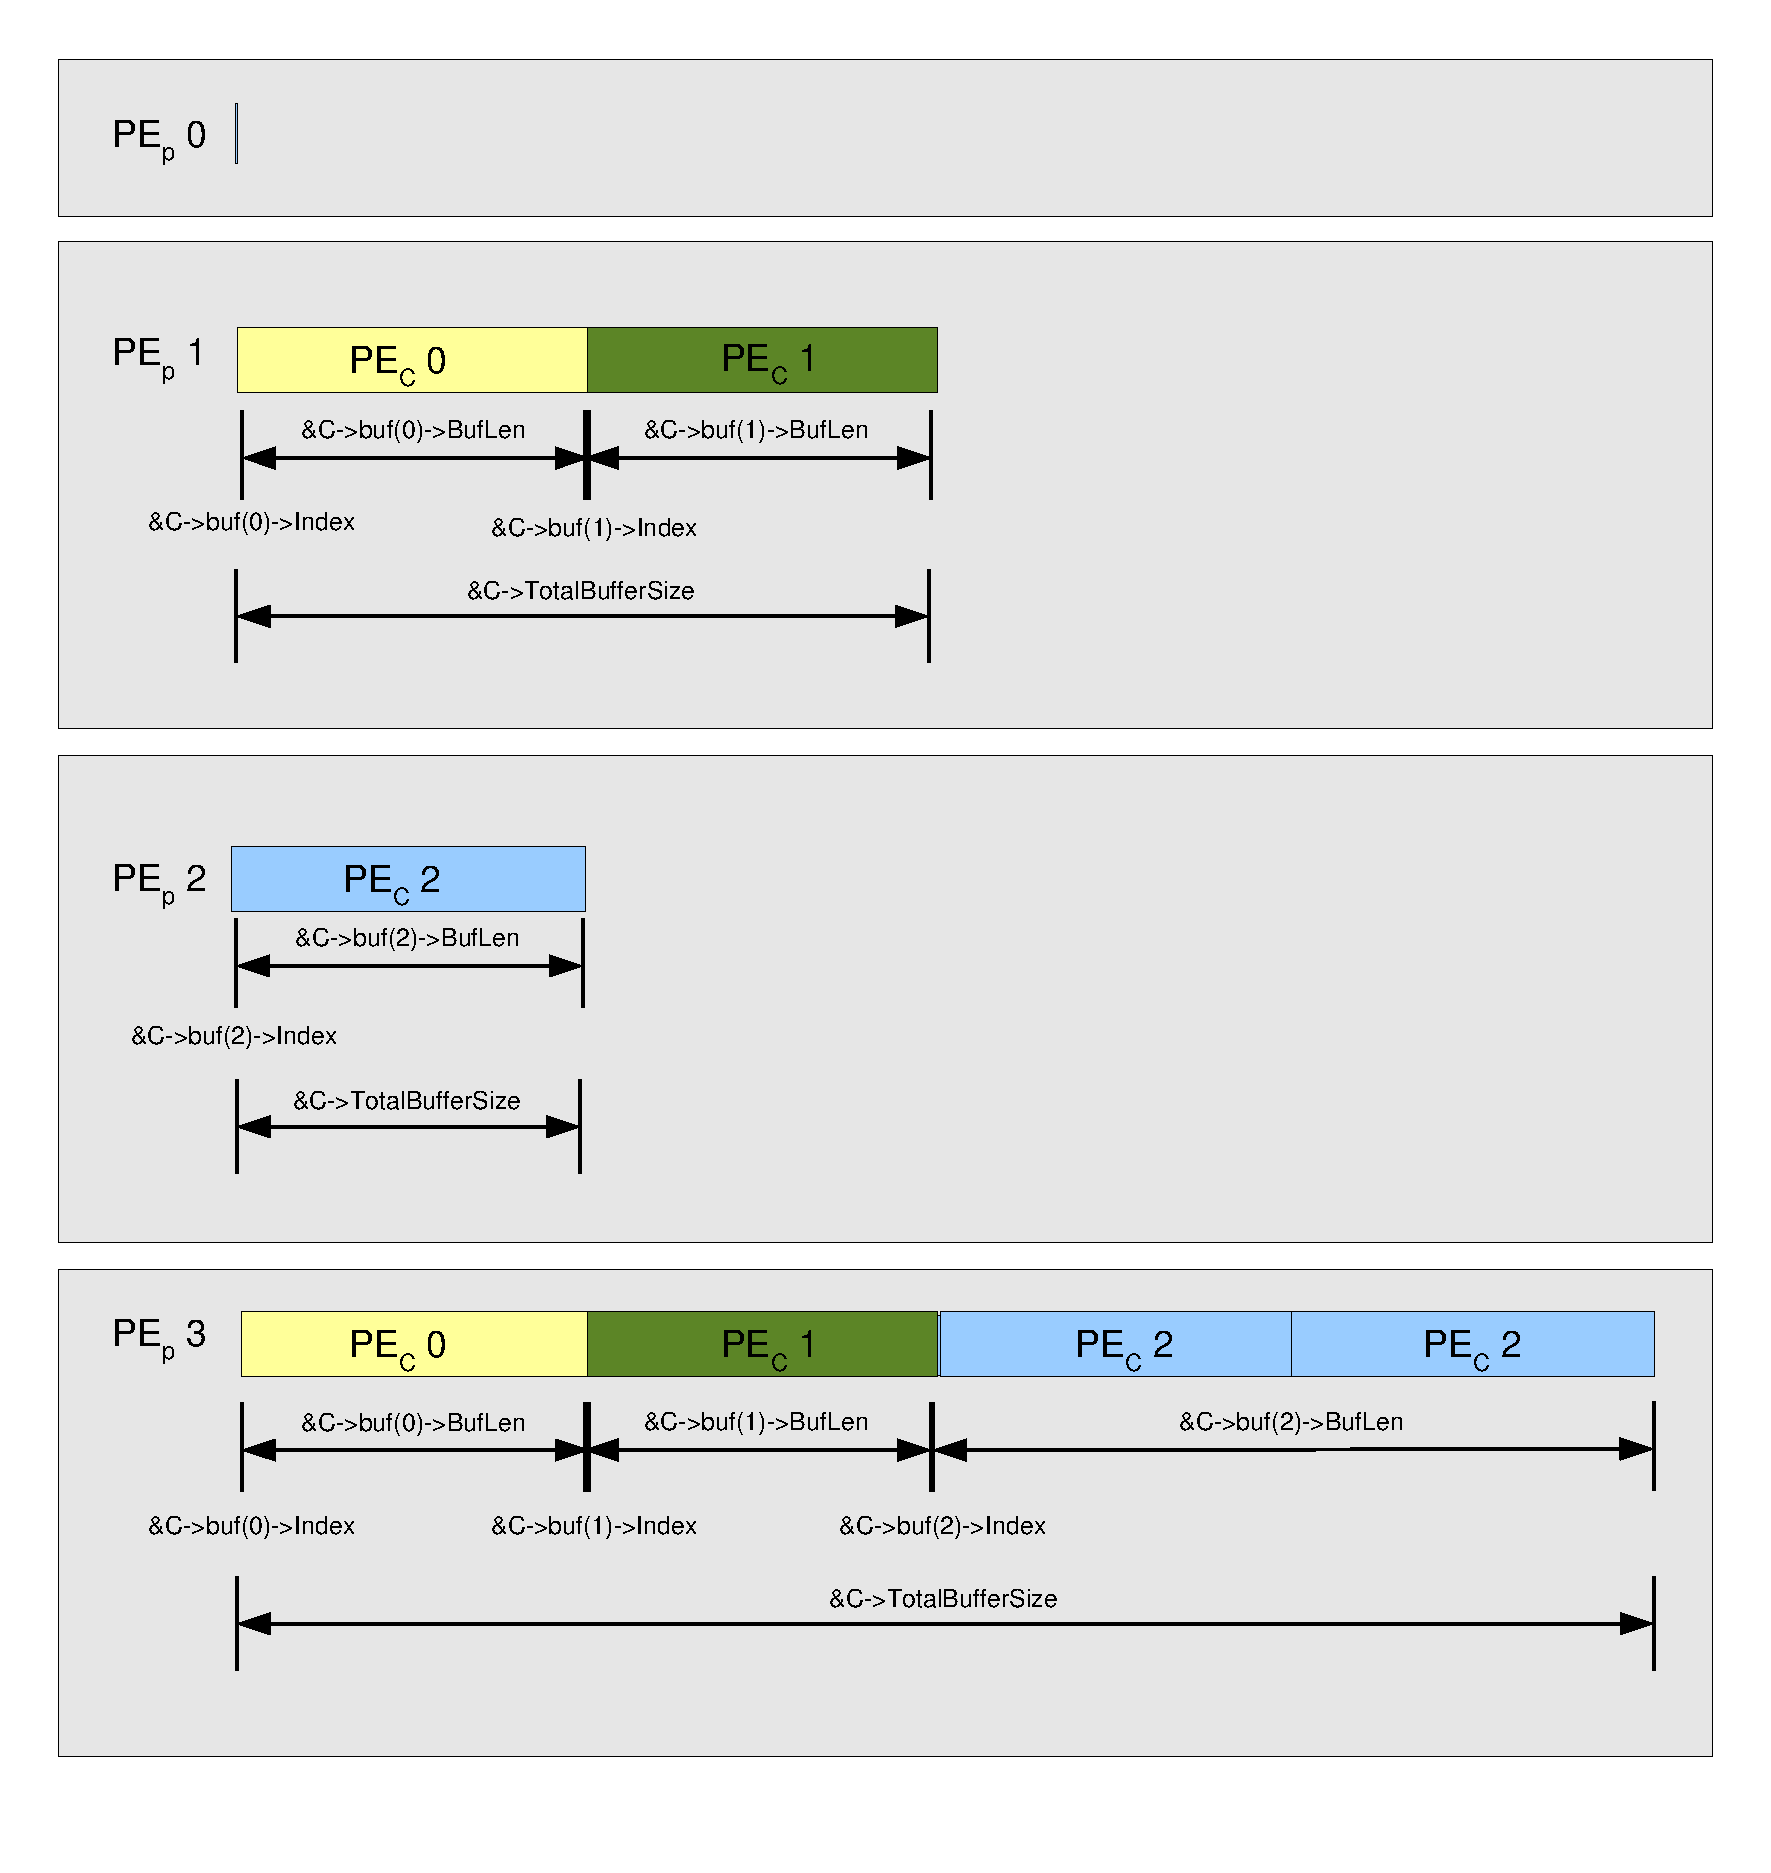
\includegraphics[width=\textwidth]{MMDlib_idxdef_server.pdf} 
\end{center} 
\vspace*{-1.5cm}
\caption{Example of a possible MMD exchange buffer layout.} 
\label{fig:idserver} 
\end{figure*} 

\begin{figure*}
\begin{center} 
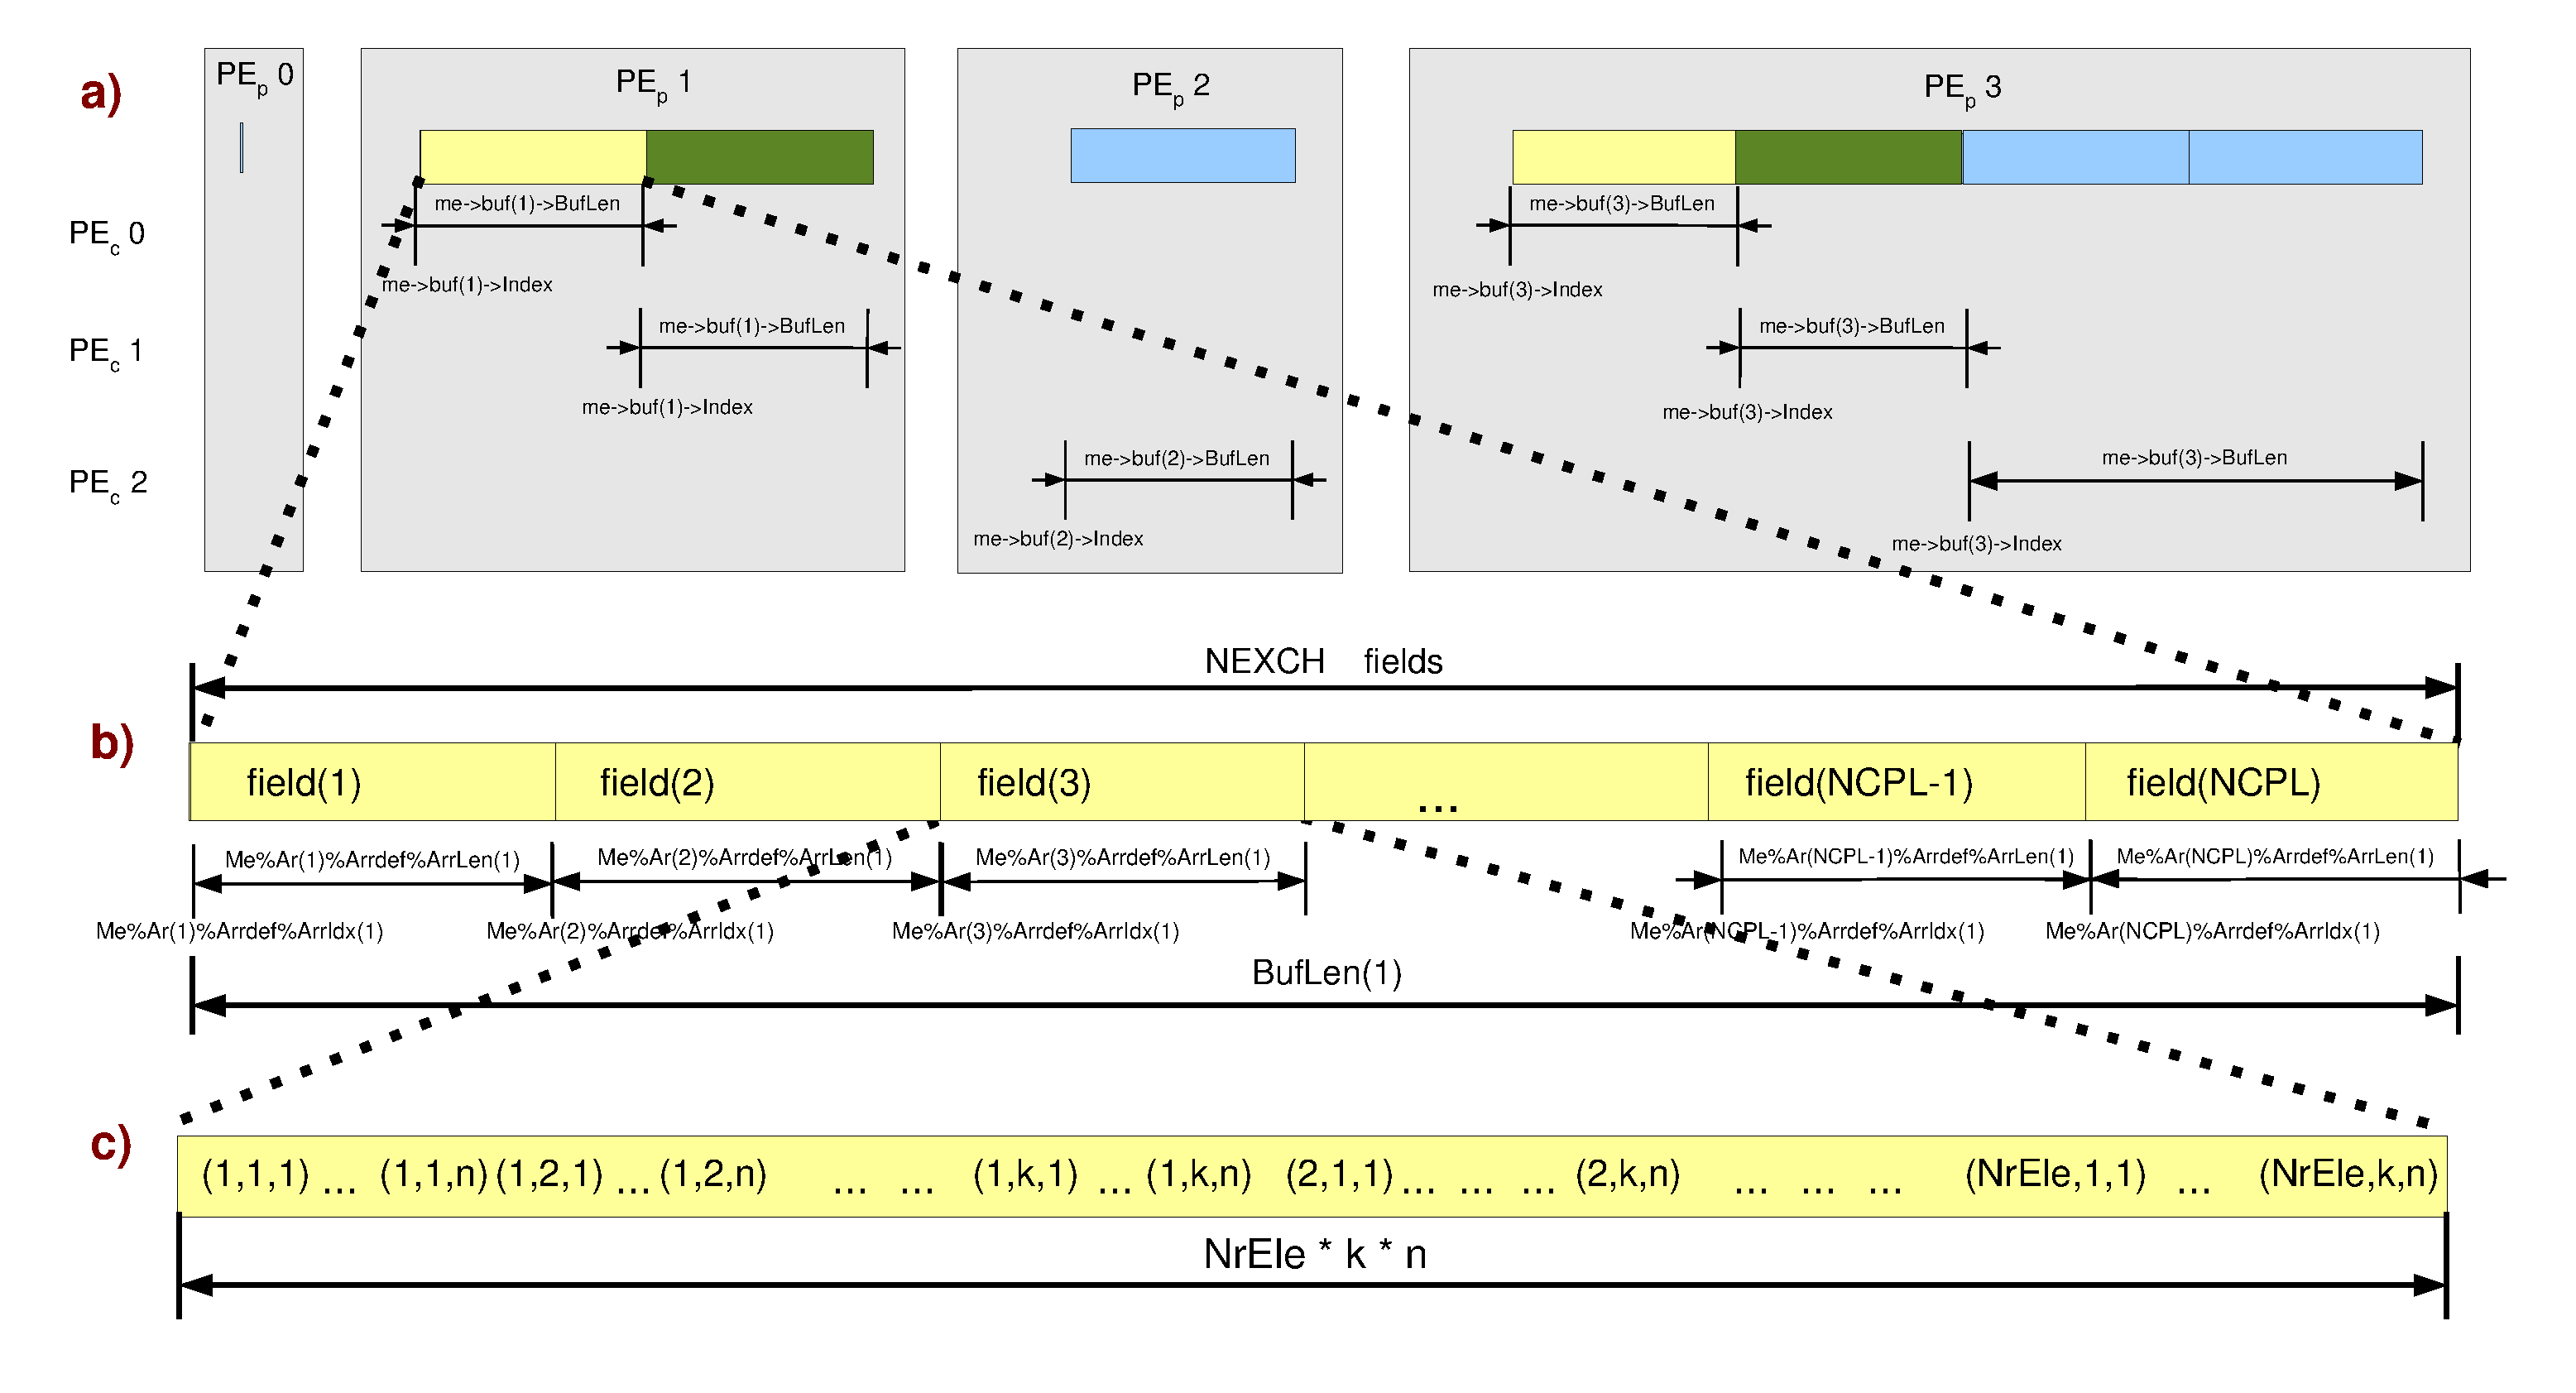
\includegraphics[angle=90, height=0.95\textheight]{MMDlib_idxdef_client.pdf} 
\end{center} 
\caption{Example of a possible MMD exchange buffer layout.} 
\label{fig:idclient} 
\end{figure*} 

In this section the meaning of the index and length variables used in the
structures are clarified with the help of the example shown in Fig.\ 
\ref{fig:MMD-NrEle} and Table \ref{tab:ex1}. The example is for the
exchange from data from the parent to one child model only. Anyhow,
the exchange in the other direction works exactly in the same way.

Figure \ref{fig:idserver} illustrates the buffer definition on the
parent model side in the C part of the library. Each grey box depicts
one parent PE. 
The first grey box is empty, as the child domain does not overlap with 
PE$_p$ 0. Parent PE$_p$ 1 contributes one grid point to child PE$_c$ 0 and one
to PE$_c$ 1. This is illustrated by the coloured bars: yellow for child PE$_c$ 0
and green for PE$_c$ 1. Each of this buffer parts is 
\verb|&Child[*ChildId-1]->buf->BufLen| long. In the figure the first part
of the structure \verb|&Child[*ChildId-1]| is abreviated by \verb|&C|.
As explained above \verb|buf| is a concatenated list. The different elements 
of this list are depicted by indices in the figure, e.g.\ ,
\verb|&C->buf(1)->BufLen| means the length of the buffer that is sent to PE$_c$ 
1.  For the correct access to the data, it must be known, where the buffers for
each of the child PEs starts. This is indicated by the respective indices
\verb|&C->buf( )->Index|. The overall length of the buffer sent by PE$_p$ 1 is
given by \verb|&C->TotalBufferSize|.

Parent PE$_p$ 2 only sends data to child PE$_c$ 2. Thus 
\verb|&C->TotalBufferSize| for PE$_p$ 2 is equal to the length of the
buffer sent 
to PE$_c$ 2 (\verb|&C->buf(2)->BufLen|). The buffer lengths attributed to the
other child PEs are set to zero.

Parent PE$_p$ 3 sends data to all three child PEs: one grid point each to 
child PE$_c$ 0 and  PE$_c$ 1 and two grid points to PE$_c$ 2. Thus 
\verb|&C->buf(2)->BufLen| is twice as large as \verb|&C->buf(0)->BufLen| or
\verb|&C->buf(1)->BufLen|.


Figure \ref{fig:idclient}a) shows the same for the child model
side. This figure part is 
constructed like a table. The parent PEs build the columns and the Child PEs 
the rows. The grey boxes indicate again the parent PEs. As PE$_p$ 0 does not
send any data, all variables are zero on all child PEs. 
Child PE$_c$ 0 receives data from PE$_p$ 1 and PE$_p$ 3. The buffer sent by
PE$_p$ 1 is \verb|me->buf(1)->BufLen| long and starts at position 
\verb|me->buf(1)->BufIndex|. Note that the index 1 of \verb|buf| referes to
 PE$_p$ 1. 
Correspondingly, the buffer received from PE$_p$ 3 starts at 
\verb|me->buf(3)->BufIndex| and its length is \verb|me->buf(3)->BufLen|.
The \verb|maxbufsize| for  PE$_c$ 0 is equal to \verb|me->buf(1)->BufLen| and
\verb|me->buf(3)->BufLen|, as they are equally long.

The respective variables for child PE$_c$ 1 are defined accordingly.
Child PE$_c$ 2 receives data from the two parent processes PE$_p$ 2 and PE$_p$ 3.
The definitions are similar, different is \verb|maxbufsize|, which is
obviously set to \verb|me->buf(3)->BufLen| as PE$_c$ 2 receives two grid points
from PE$_p$ 3 but only one from PE$_p$ 2.

The C part needs to deal only with the buffers exchanged between
one parent and one child PE. While this part is illustrated in Fig.\ 
\ref{fig:idclient}a), parts  \ref{fig:idclient}b) and  \ref{fig:idclient}c) of
 the figure deal with the variable
definitions in the Fortran95 part of the library, where the single exchanged 
fields (Fig.\ \ref{fig:idclient}b) and individual horizontal grid elements
 of each field (Fig.\ \ref{fig:idclient}c) are addressed.

 Figure \ref{fig:idclient}b) illustrates the order of the single fields within
one buffer dealt with by C. Per exchanged buffer (i.e., per child and
per parent PE) the fields are stored one after the other in the order
of their definition. The number of fields is always the full number of {\it 
exchange fields} (\verb|NEXCH|). 
The length of the individual fields can vary, as the vertical
and the number dimension can differ\footnote{Note: the horizontal dimensions 
must be the same for all fields exchanged between one Parent and one Child PE,
 i.e., {\tt Me\%PEs(ip)\%NrEle}.}. 
The individual length of each field is saved in the 
variable \verb|Child(Id)%Ar(ix)%Arrdef%ArrLen(ip)|. Where \verb|ix| is the number of
the field. This is again a pseudo-index used for illustration, as \verb|Child(Id)%Ar|
is a concatenated list. The index \verb|ip| indicates the respective parent PE.
\verb|Me%Ar(ix)%Arrdef%ArrLen(ip)| can be different for each parent PE, because
the number of elements exchanged with each parent PE (\verb|Me%PEs(ip)%NrEle|) 
can be different for each parent PE.
As the array lengths can vary, the start index of each of the fields within
the exchanged buffer is saved in the variable \verb|Me%Ar(ix)%Arrdef%ArrIdx|.
 \verb|BufLen(ip)| in \verb|mmd_child.f90| is  defined as the sum
over \verb|ix| in \verb|Me%Ar(ix)%Arrdef%ArrLen(ip)|.  \verb|BufLen(ip)| equals
\verb|me->buf(ip)->BufLen| in \verb|mmdc_client.c|.

 Figure \ref{fig:idclient}c) shows the sequence of the single data points of
one field as aligned by the packing algorithm.
 The fastest varying index is the number dimension (\verb|n|), 
the second fastest is the vertical dimension (\verb|k|). The horizontal 
dimension (from 1 to \verb|NrEle|) varies most slowly.

\begin{appendix}
\section{\noindent Glossary}
\begin{itemize}
\item {\it attributes}: {\it Attributes} represent time independent, scalar 
characteristics, e.g., the measuring unit.
\item {\it axis string}: It is a \footnotesize{CHARACTER} of length 4, it
is defined for each {\it representation}, indicating which rank is associated
to which dimension. For instance, 'XY--' indicates a horizontal 2D field in
grid point space. 
\item {\it channel}: The generic submodel CHANNEL manages the 
memory and meta-data and provides a data transfer and export interface.
A {\it channel} represents sets of ``related'' {\it channel objects}
with additional meta information. The ``relation'' can be, for instance, the 
simple fact that the {\it channel objects} are defined by the same submodel.
\item {\it channel object}: It represents a data field including
its meta information and its underlying
geometric structure ({\it representation}), e.g., the 3-dimensional vorticity in
 spectral {\it representation}, the ozone mixing ratio in Eulerian 
{\it representation}, the pressure altitude of trajectories in Lagrangian 
{\it representation}.
\item {\it dimensions}: They represent the basic geometry of one dimension,
e.g., the number of latitude points, the number of trajectories, etc.
\item {\it exchange field}: An {\it exchange field} is a field requested within 
  the \verb|&CPL_CHILD_ECHAM| or \verb|&CPL_CHILD_COSMO| namelist in
  the \verb|mmd2way.nml| namelist file and provided by the parent to
  the child.  
  An {\it exchange field} can either be a field which is remapped and copied
  to a child variable, or a field required for the 
  grid mapping itself.

  For the 2-way coupling the term is also used for the fields the
  parent receives from the child model.
\item {\it in-field}: The {\it in-fields} are those fields provided by 
  the parent or {\it driving model}, which are still defined on the parent grid,
  but on the child side. In other words, {\it in-fields} are the
  {\it exchanged fields} before the grid mapping.
  
  For the 2-way coupling this term is also used for the fields
  received by the parent model. In this case the field have already
  been mapped to the parent grid, but these fields are only
  defined on the exchanged area.
\item {\it in-grid}: grid on which the {\it in-fields} are defined.
\item {\it master parent}: The {\it master parent} or {\it patriarch}
  is the coarsest model in a  model cascade, i.e., that model that has
  no parent model itself. In the MMD library 
namelist this model is indicated by a ``-1'' as associated parent model.
 In most cases this is a global model.  The {\it patriarch}
determines the time setting of the entire model cascade. 
\item {\it out-grid}: The {\it out-grid} is a subpart of the parent model
  grid, defined by the child submodel MMD2WAY\_CHILD. This is the
  target grid for the remapping of the child model fields to the parent 
  grid before the remapped data is sent back to the parent. 
\item {\it patriarch}: The {\it patriarch} or {\it master parent} 
  is the coarsest model in a  model cascade, i.e., that model that has
  no parent model itself. In the MMD library 
namelist this model is indicated by a ``-1'' as associated parent model.
 In most cases this is a global model.  The {\it patriarch}
determines the time setting of the entire model cascade. 
\item {\it Receiver}: short for {\it receiving model}
\item {\it receiving model}: the model receiving the data. In case of
1-way coupling the child model (client) is always the {\it receiving
model}, while the parent model (server) is always the {\it sending model}.

\item {\it remote model}: the ``other'' model in a communicating
child-parent model 
pair; i.e., for the child the parent, for the parent the respective child
\item {\it remote PE}: the ``other'' PE in a pair of child and parent
model PEs exchanging data. For example, parent PE$_p$ 2 is sending
data to child PE$_c$ 4: 
in this case PE$_c$ 4 is the {\it remote PE} for parent PE$_p$ 2 and
vice versa. 
\item {\it representation}: It describes multidimensional geometric
structures (based on {\it dimensions}), e.g., Eulerian (or grid point),
spectral, Lagrangian.
%\item {\it rerun event}: It triggers the output of {\it restart files}.
\item {\it Sender}: short for {\it sending model}
\item {\it sending model}: the model sending the data. In case of
1-way coupling the child (client) model is always the {\it receiving
model}, while the parent (server) model is always the {\it sending model}.

\end{itemize}

\end{appendix}

\bibliographystyle{copernicus} % bst file
\bibliography{MMDlib}       % bib files

\end{document}
